
\documentclass{WileyMSP-template}
\usepackage{graphicx}
\usepackage{booktabs}
\usepackage{adjustbox}
\usepackage{longtable}
\usepackage{pdflscape}
\usepackage{caption}
\begin{document}
\title{Supplementary Information \\Attention-based pattern discovery of mass spectrometry imaging data}
\maketitle
\begin{figure}[htbp]
  \centering
  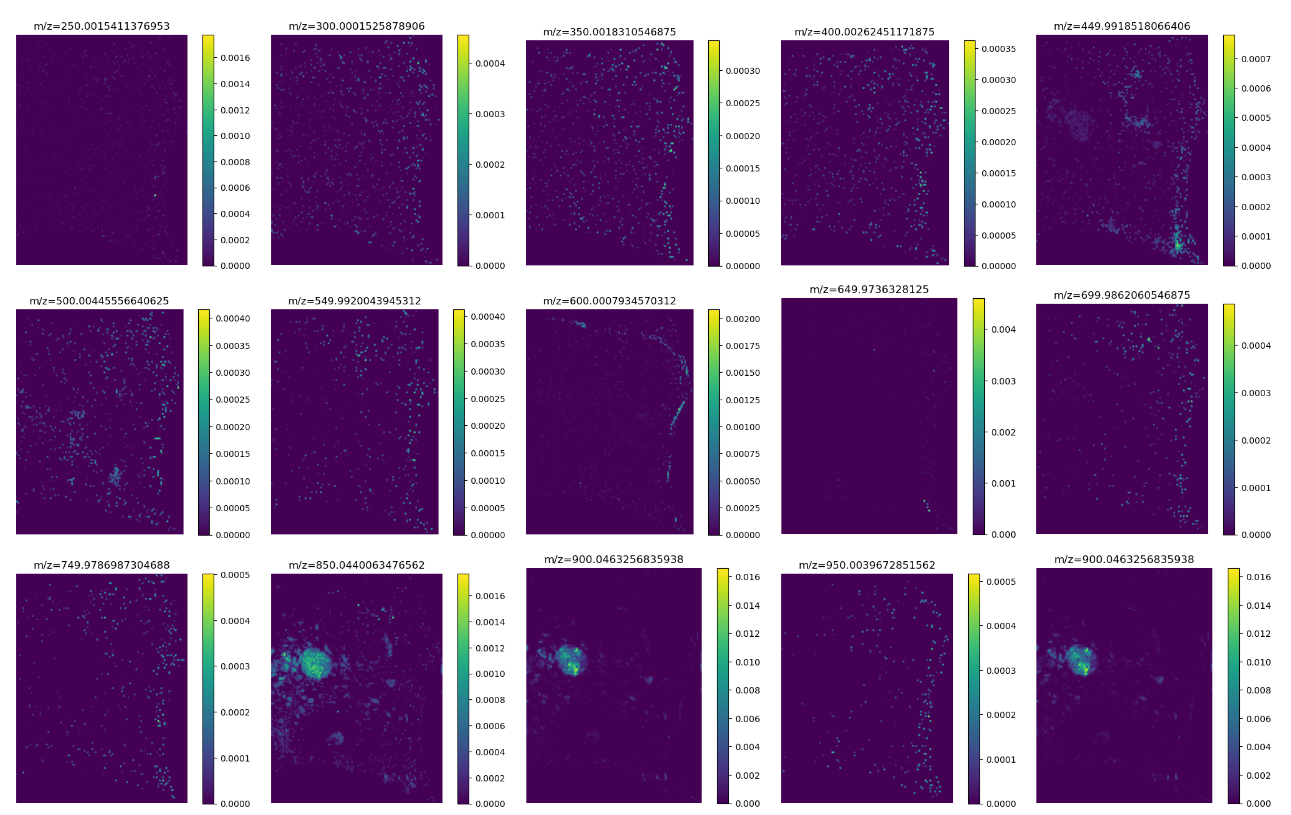
\includegraphics[width=\linewidth]{pic/prostate/several_mz.png}
  \captionsetup{justification=raggedright,singlelinecheck=false}
  \caption 
  {
    \textbf{Several patterns of MSI data from prostate cancer tissues}.
    It is readily apparent that at most m/z channels, the intensity of MSI 
    is faint and disorganized. Such raw data cannot be directly utilized 
    for subsequent analysis. 
    Conventional approaches involve dimensionality reduction and manual 
    selection of specific m/z channels. 
  }
  \label{fig:Several patterns of prostate tissue} 
\end{figure}

\begin{landscape}
    \thispagestyle{empty}
    \begin{table}
        \centering
        \begin{adjustbox}{center}
            \resizebox{0.99\pdfpageheight}{!}{
            \centering 
            \begin{tabular}{|c|c|c|c|c|c|c|c|c|c|c|c|c|}
            \toprule
            % m/z & Name & Compound Name & Formula & Class & Pathways & Score & Adduct & Exact Mass & Error & Database & Accession \\
            % \midrule
            % 774.5983 & PC(15:020:1(11Z)) & 1-Pentadecanoyl-2-eicosenoyl-sn-glycero-3-phosphocholine 
            % & $ C_{43}H_{84}NO_{8}P $ & Phosphatidylcholines & 1. Phosphatidylcholine Biosynthesis 2. Phosphatidylethanolamine Biosynthesis  
            % & M+H & 774.6007312 & 3.138649245 & HMDB & HMDB07945 & HMDB07945 \\

            % 774.5983 &	PC(20:1(11Z)15:0)&	1-Eicosenoyl-2-pentadecanoyl-sn-glycero-3-phosphocholine
            % &$ C_{43}H_{84}NO_{8}P $&	Phosphatidylcholines&	1. Phosphatidylcholine Biosynthesis 2. Phosphatidylethanolamine Biosynthesis 
            % &M+H	&774.6007312&	3.138649245	&HMDB	&HMDB08297&	HMDB08297 \\

            % 774.5983 & PE(14:024:1(15Z)) & 1-Myristoyl-2-nervonoyl-sn-glycero-3-phosphoethanolamine 
            % & $ C_{43}H_{84}NO_{8}P $ & Phosphatidylethanolamines & 1. Phosphatidylcholine Biosynthesis 2. Phosphatidylethanolamine Biosynthesis 
            % & M+H & 774.6007312 & 3.138649245 & HMDB & HMDB08849 & HMDB08849 \\

            % 774.5983 & PE(14:1(9Z)24:0) & 1-Myristoleoyl-2-lignoceroyl-sn-glycero-3-phosphoethanolamine 
            % & $ C_{43}H_{84}NO_{8}P $ & Phosphatidylethanolamines & 1. Phosphatidylcholine Biosynthesis 2. Phosphatidylethanolamine Biosynthesis 
            % & M+H & 774.6007312 & 3.138649245 & HMDB & HMDB08881 & HMDB08881 \\

            % 774.5983 & PE(16:022:1(13Z)) & 1-Palmitoyl-2-erucoyl-sn-glycero-3-phosphoethanolamine 
            % & $ C_{43}H_{84}NO_{8}P $ & Phosphatidylethanolamines & 1. Phosphatidylcholine Biosynthesis 2. Phosphatidylethanolamine Biosynthesis 
            % & M+H & 774.6007312 & 3.138649245 & HMDB & HMDB08941 & HMDB08941 \\

            % 774.5983 & PE(16:1(9Z)22:0) & 1-Palmitoleoyl-2-behenoyl-sn-glycero-3-phosphoethanolamine
            % & $ C_{43}H_{84}NO_{8}P $ & Phosphatidylethanolamines & 1. Phosphatidylcholine Biosynthesis 2. Phosphatidylethanolamine Biosynthesis
            % & M+H & 774.6007312 & 3.138649245 & HMDB & HMDB08973 & HMDB08973 \\

            % 774.5983 & PE(18:020:1(11Z)) & 1-Stearoyl-2-eicosenoyl-sn-glycero-3-phosphoethanolamine 
            % & $ C_{43}H_{84}NO_{8}P $ & Phosphatidylethanolamines & 1. Phosphatidylcholine Biosynthesis 2. Phosphatidylethanolamine Biosynthesis 
            % & M+H & 774.6007312 & 3.138649245 & HMDB & HMDB08999 & HMDB08999 \\

            % 774.5983 & PE(18:1(11Z)20:0) & 1-Vaccenoyl-2-arachidonyl-sn-glycero-3-phosphoethanolamine 
            % & $ C_{43}H_{84}NO_{8}P $ & Phosphatidylethanolamines & 1. Phosphatidylcholine Biosynthesis 2. Phosphatidylethanolamine Biosynthesis 
            % & M+H & 774.6007312 & 3.138649245 & HMDB & HMDB09031 & HMDB09031 \\

            % 774.5983 & PE(18:1(9Z)20:0) & 1-Oleoyl-2-arachidonyl-sn-glycero-3-phosphoethanolamine
            %  & $ C_{43}H_{84}NO_{8}P $ & Phosphatidylethanolamines & 1. Phosphatidylcholine Biosynthesis 2. Phosphatidylethanolamine Biosynthesis 
            % & M+H & 774.6007312 & 3.138649245 & HMDB & HMDB09064 & HMDB09064 \\

            % 774.5983 & PE(20:018:1(11Z)) & 1-Arachidonyl-2-vaccenoyl-sn-glycero-3-phosphoethanolamine 
            % & $ C_{43}H_{84}NO_{8}P $ & Phosphatidylethanolamines & 1. Phosphatidylcholine Biosynthesis 2. Phosphatidylethanolamine Biosynthesis 
            % & M+H & 774.6007312 & 3.138649245 & HMDB & HMDB09223 & HMDB09223 \\
            
            % 774.5983 & PE(20:018:1(9Z)) & 1-Arachidonyl-2-oleoyl-sn-glycero-3-phosphoethanolamine 
            % & $ C_{43}H_{84}NO_{8}P $ & Phosphatidylethanolamines & 1. Phosphatidylcholine Biosynthesis 2. Phosphatidylethanolamine Biosynthesis 
            % & M+H & 774.6007312 & 3.138649245 & HMDB & HMDB09224 & HMDB09224 \\

            % 774.5983 & PE(20:1(11Z)18:0) & 1-Eicosenoyl-2-stearoyl-sn-glycero-3-phosphoethanolamine 
            % & $ C_{43}H_{84}NO_{8}P $ & Phosphatidylethanolamines & 1. Phosphatidylcholine Biosynthesis 2. Phosphatidylethanolamine Biosynthesis 
            % & M+H & 774.6007312 & 3.138649245 & HMDB & HMDB09255 & HMDB09255 \\

            % 774.5983 & PE(22:016:1(9Z)) & 1-Behenoyl-2-palmitoleoyl-sn-glycero-3-phosphoethanolamine
            %  & $ C_{43}H_{84}NO_{8}P $ & Phosphatidylethanolamines & 1. Phosphatidylcholine Biosynthesis 2. Phosphatidylethanolamine Biosynthesis
            %  & M+H & 774.6007312 & 3.138649245 & HMDB & HMDB09485 & HMDB09485 \\

            %  774.5983 & PE(22:1(13Z)16:0) & 1-Erucoyl-2-palmitoyl-sn-glycero-3-phosphoethanolamine 
            %  & $ C_{43}H_{84}NO_{8}P $ & Phosphatidylethanolamines & 1. Phosphatidylcholine Biosynthesis 2. Phosphatidylethanolamine Biosynthesis
            %   & M+H & 774.6007312 & 3.138649245 & HMDB & HMDB09517 & HMDB09517 \\

            %   774.5983 & PE(24:014:1(9Z)) & 1-lignoceroyl-2-myristoleoyl-sn-glycero-3-phosphoethanolamine 
            %   & $ C_{43}H_{84}NO_{8}P $ & Phosphatidylethanolamines & 1. Phosphatidylcholine Biosynthesis 2. Phosphatidylethanolamine Biosynthesis 
            %   & M+H & 774.6007312 & 3.138649245 & HMDB & HMDB09713 & HMDB09713 \\

            %   774.5983 & PE(24:1(15Z)14:0) & 1-Nervonoyl-2-myristoyl-sn-glycero-3-phosphoethanolamine 
            %   & $ C_{43}H_{84}NO_{8}P $ & Phosphatidylethanolamines & 1. Phosphatidylcholine Biosynthesis 2. Phosphatidylethanolamine Biosynthesis 
            %   & M+H & 774.6007312 & 3.138649245 & HMDB & HMDB09745 & HMDB09745 \\
            % \bottomrule

            %  884.5723 \\
            % \bottomrule
            %  845.6712 & PE(18:1(11Z)24:1(15Z)) & 1-Vaccenoyl-2-nervonoyl-sn-glycero-3-phosphoethanolamine 
            %  & $ C_{47}H_{90}NO_{8}P $ & Phosphatidylethanolamines & 1. Phosphatidylcholine Biosynthesis 2. Phosphatidylethanolamine Biosynthesis 
            %  & M+NH4 & 845.6742284 & 3.581047995 & HMDB & HMDB09047 & HMDB09047 \\

            %  845.6712 & PE(18:1(9Z)24:1(15Z)) & 1-Oleoyl-2-nervonoyl-sn-glycero-3-phosphoethanolamine 
            %  & $ C_{47}H_{90}NO_{8}P $ & Phosphatidylethanolamines & 1. Phosphatidylcholine Biosynthesis 2. Phosphatidylethanolamine Biosynthesis 
            %  & M+NH4 & 845.6742284 & 3.581047995 & HMDB & HMDB09080 & HMDB09080 \\

            %  845.6712 & PE(18:2(9Z12Z)24:0) & 1-Linoleoyl-2-lignoceroyl-sn-glycero-3-phosphoethanolamine 
            %  & $ C_{47}H_{90}NO_{8}P $ & Phosphatidylethanolamines & 1. Phosphatidylcholine Biosynthesis 2. Phosphatidylethanolamine Biosynthesis 
            %  & M+NH4 & 845.6742284 & 3.581047995 & HMDB & HMDB09112 & HMDB09112 \\

            %  845.6712 & PE(20:022:2(13Z16Z)) & 1-Arachidonyl-2-docosadienoyl-sn-glycero-3-phosphoethanolamine 
            %  & $ C_{47}H_{90}NO_{8}P $ & Phosphatidylethanolamines & 1. Phosphatidylcholine Biosynthesis 2. Phosphatidylethanolamine Biosynthesis 
            %  & M+NH4 & 845.6742284 & 3.581047995 & HMDB & HMDB09239 & HMDB09239 \\
            
            %  845.6712 & PE(20:1(11Z)22:1(13Z)) & 1-Eicosenoyl-2-erucoyl-sn-glycero-3-phosphoethanolamine 
            %  & $ C_{47}H_{90}NO_{8}P $ & Phosphatidylethanolamines & 1. Phosphatidylcholine Biosynthesis 2. Phosphatidylethanolamine Biosynthesis 
            %  & M+NH4 & 845.6742284 & 3.581047995 & HMDB & HMDB09271 & HMDB09271 \\

            %  845.6712 & PE(20:2(11Z14Z)22:0) & 1-Eicosadienoyl-2-behenoyl-sn-glycero-3-phosphoethanolamine 
            %  & $ C_{47}H_{90}NO_{8}P $ & Phosphatidylethanolamines & 1. Phosphatidylcholine Biosynthesis 2. Phosphatidylethanolamine Biosynthesis 
            %  & M+NH4 & 845.6742284 & 3.581047995 & HMDB & HMDB09303 & HMDB09303 \\

            %  845.6712 & PE(22:020:2(11Z14Z)) & 1-Behenoyl-2-eicosadienoyl-sn-glycero-3-phosphoethanolamine 
            %  & $ C_{47}H_{90}NO_{8}P $ & Phosphatidylethanolamines & 1. Phosphatidylcholine Biosynthesis 2. Phosphatidylethanolamine Biosynthesis 
            %  & M+NH4 & 845.6742284 & 3.581047995 & HMDB & HMDB09495 & HMDB09495 \\

            %  845.6712 & PE(22:1(13Z)20:1(11Z)) & 1-Erucoyl-2-eicosenoyl-sn-glycero-3-phosphoethanolamine 
            %  & $ C_{47}H_{90}NO_{8}P $ & Phosphatidylethanolamines & 1. Phosphatidylcholine Biosynthesis 2. Phosphatidylethanolamine Biosynthesis 
            %  & M+NH4 & 845.6742284 & 3.581047995 & HMDB & HMDB09527 & HMDB09527 \\

            %  845.6712 & PE(22:2(13Z16Z)20:0) & 1-Docosadienoyl-2-arachidonyl-sn-glycero-3-phosphoethanolamine 
            %  & $ C_{47}H_{90}NO_{8}P $ & Phosphatidylethanolamines & 1. Phosphatidylcholine Biosynthesis 2. Phosphatidylethanolamine Biosynthesis 
            %  & M+NH4 & 845.6742284 & 3.581047995 & HMDB & HMDB09559 & HMDB09559 \\

            %  845.6712 & PE(24:018:2(9Z12Z)) & 1-Lignoceroyl-2-linoleoyl-sn-glycero-3-phosphoethanolamine 
            %  & $ C_{47}H_{90}NO_{8}P $ & Phosphatidylethanolamines & 1. Phosphatidylcholine Biosynthesis 2. Phosphatidylethanolamine Biosynthesis 
            %  & M+NH4 & 845.6742284 & 3.581047995 & HMDB & HMDB09720 & HMDB09720 \\

            %  845.6712 & PE(24:1(15Z)18:1(11Z)) & 1-nervonoyl-2-vaccenoyl-sn-glycero-3-phosphoethanolamine 
            %  & $ C_{47}H_{90}NO_{8}P $ & Phosphatidylethanolamines & 1. Phosphatidylcholine Biosynthesis 2. Phosphatidylethanolamine Biosynthesis 
            %  & M+NH4 & 845.6742284 & 3.581047995 & HMDB & HMDB09751 & HMDB09751 \\

            %  845.6712 & PE(24:1(15Z)18:1(9Z)) & 1-nervonoyl-2-oleoyl-sn-glycero-3-phosphoethanolamine 
            %  & $ C_{47}H_{90}NO_{8}P $ & Phosphatidylethanolamines & 1. Phosphatidylcholine Biosynthesis 2. Phosphatidylethanolamine Biosynthesis 
            %  & M+NH4 & 845.6742284 & 3.581047995 & HMDB & HMDB09752 & HMDB09752 \\
            % \bottomrule
            % 775.6025 \\
            % \bottomrule
            % 760.5827 & PC(14:020:1(11Z)) & 1-Myristoyl-2-eicosenoyl-sn-glycero-3-phosphocholine & $ C_{42}H_{82}NO_{8}P $ & Phosphatidylcholines & 1. Phosphatidylcholine Biosynthesis 2. Phosphatidylethanolamine Biosynthesis & M+H & 760.5850811 & 3.130616231 & HMDB & HMDB07879 & HMDB07879 \\
            % 760.5827 & PC(14:1(9Z)20:0) & 1-Myristoleoyl-2-arachidonyl-sn-glycero-3-phosphocholine & $ C_{42}H_{82}NO_{8}P $ & Phosphatidylcholines & 1. Phosphatidylcholine Biosynthesis 2. Phosphatidylethanolamine Biosynthesis & M+H & 760.5850811 & 3.130616231 & HMDB & HMDB07911 & HMDB07911 \\
            % 760.5827 & PC(16:018:1(11Z)) & 1-Palmitoyl-2-vaccenoyl-sn-glycero-3-phosphocholine & $ C_{42}H_{82}NO_{8}P $ & Phosphatidylcholines & 1. Phosphatidylcholine Biosynthesis 2. Phosphatidylethanolamine Biosynthesis & M+H & 760.5850811 & 3.130616231 & HMDB & HMDB07971 & HMDB07971 \\
            % 760.5827 & PC(16:018:1(9Z)) & 1-Hexadecanoyl-2-oleoyl-sn-glycero-3-phosphocholine & $ C_{42}H_{82}NO_{8}P $ & Phosphatidylcholines & 1. Phosphatidylcholine Biosynthesis 2. Phosphatidylethanolamine Biosynthesis & M+H & 760.5850811 & 3.130616231 & HMDB & HMDB07972 & HMDB07972 \\
            % 760.5827 & PC(16:1(9Z)18:0) & 1-(9Z-Hexadecenoyl)-2-octadecanoyl-sn-glycero-3-phosphocholine & $ C_{42}H_{82}NO_{8}P $ & Phosphatidylcholines & 1. Phosphatidylcholine Biosynthesis 2. Phosphatidylethanolamine Biosynthesis & M+H & 760.5850811 & 3.130616231 & HMDB & HMDB08003 & HMDB08003 \\
            % 760.5827 & PC(18:016:1(9Z)) & 1-Stearoyl-2-palmitoleoyl-sn-glycero-3-phosphocholine & $ C_{42}H_{82}NO_{8}P $ & Phosphatidylcholines & 1. Phosphatidylcholine Biosynthesis 2. Phosphatidylethanolamine Biosynthesis & M+H & 760.5850811 & 3.130616231 & HMDB & HMDB08035 & HMDB08035 \\
            % 760.5827 & PC(18:1(11Z)16:0) & 1-Vaccenoyl-2-palmitoyl-sn-glycero-3-phosphocholine & $ C_{42}H_{82}NO_{8}P $ & Phosphatidylcholines & 1. Phosphatidylcholine Biosynthesis 2. Phosphatidylethanolamine Biosynthesis & M+H & 760.5850811 & 3.130616231 & HMDB & HMDB08067 & HMDB08067 \\
            % 760.5827 & PC(18:1(9Z)16:0) & 1-Palmotoyl-2-oleoylglycero-3-phosphocholine & $ C_{42}H_{82}NO_{8}P $ & Phosphatidylcholines & 1. Phosphatidylcholine Biosynthesis 2. Phosphatidylethanolamine Biosynthesis & M+H & 760.5850811 & 3.130616231 & HMDB & HMDB08100 & HMDB08100 \\
            % 760.5827 & PC(20:014:1(9Z)) & 1-arachidonyl-2-myristoleoyl-sn-glycero-3-phosphocholine & $ C_{42}H_{82}NO_{8}P $ & Phosphatidylcholines & 1. Phosphatidylcholine Biosynthesis 2. Phosphatidylethanolamine Biosynthesis & M+H & 760.5850811 & 3.130616231 & HMDB & HMDB08263 & HMDB08263 \\
            % 760.5827 & PC(20:1(11Z)14:0) & 1-Eicosenoyl-2-myristoyl-sn-glycero-3-phosphocholine & $ C_{42}H_{82}NO_{8}P $ & Phosphatidylcholines & 1. Phosphatidylcholine Biosynthesis 2. Phosphatidylethanolamine Biosynthesis & M+H & 760.5850811 & 3.130616231 & HMDB & HMDB08295 & HMDB08295 \\
            % 760.5827 & PE(15:022:1(13Z)) & 1-Pentadecanoyl-2-erucoyl-sn-glycero-3-phosphoethanolamine & $ C_{42}H_{82}NO_{8}P $ & Phosphatidylethanolamines & 1. Phosphatidylcholine Biosynthesis 2. Phosphatidylethanolamine Biosynthesis & M+H & 760.5850811 & 3.130616231 & HMDB & HMDB08908 & HMDB08908 \\
            % 760.5827 & PE(22:1(13Z)15:0) & 1-Erucoyl-2-pentadecanoyl-sn-glycero-3-phosphoethanolamine & $ C_{42}H_{82}NO_{8}P $ & Phosphatidylethanolamines & 1. Phosphatidylcholine Biosynthesis 2. Phosphatidylethanolamine Biosynthesis & M+H & 760.5850811 & 3.130616231 & HMDB & HMDB09516 & HMDB09516 \\
            % \bottomrule
            % 761.5867 & NA & Termitomycesphin A & $ C_{41}H_{77}NO_{10} $ & Neutral glycosphingolipids & NA & M+NH4 & 761.588573 & 2.459333118 & Lipidmaps & NA & LMSP01080015 \\
            % 829.6375 & NA & NA & NA & NA & NA & NA & NA & NA & NA & NA & NA \\
            % 863.6799 & 3-O-(6-O-(11Z14Z17Z-eicosatrienoyl)-beta-D-glucopyranosyl)-stigmast-522E-dien-3beta-ol & 3-O-(6'-O-(11Z,14Z,17Z-eicosatrienoyl)-beta-D-glucopyranosyl)-stigmast-5,22E-dien-3beta-ol & $ C_{55}H_{90}O_{7} $ & Sterols  & NA & M+H & 863.675933 & 4.593157976 & Lipidmaps & NA & LMST01040233 \\
            % 803.6224 & NA & NA & NA & NA & NA & NA & NA & NA & NA & NA & NA \\
            % 504.3485 & NA & NA & NA & NA & NA & NA & NA & NA & NA & NA & NA \\
            % 846.677 & NA & NA & NA & NA & NA & NA & NA & NA & NA & NA & NA \\
            % 762.5862 & N-(docosanoyl)-1-beta-glucosyl-4E6E-pentadecasphingadienine & N-(docosanoyl)-1-beta-glucosyl-4E,6E-pentadecasphingadienine & $ C_{43}H_{81}NO_{8} $ & Neutral glycosphingolipids & NA & M+Na & 762.585438 & 0.999232298 & Lipidmaps & NA & LMSP0501AA60 \\
            % 864.6829 & NA & NA & NA & NA & NA & NA & NA & NA & NA & NA & NA \\
            % 253.5388 & NA & NA & NA & NA & NA & NA & NA & NA & NA & NA & NA \\
            % 804.6077 & 1-hexadecyl-2-(11Z-docosenoyl)-glycero-3-phosphoserine & 1-hexadecyl-2-(11Z-docosenoyl)-glycero-3-phosphoserine & $ C_{44}H_{86}NO_{9}P $ & Glycerophospholipids & NA &M+H & 804.611299 & 4.472967263 & Lipidmaps & NA & LMGP03020015 \\
            % 804.6077 & 1-octadecyl-2-(11Z-eicosenoyl)-glycero-3-phosphoserine & 1-octadecyl-2-(11Z-eicosenoyl)-glycero-3-phosphoserine & $ C_{44}H_{86}NO_{9}P $ & Glycerophospholipids & NA & M+H & 804.611299 & 4.472967263 & Lipidmaps & NA & LMGP03020034 \\
            % 804.6077 & 1-eicosyl-2-(9Z-octadecenoyl)-glycero-3-phosphoserine & 1-eicosyl-2-(9Z-octadecenoyl)-glycero-3-phosphoserine & $ C_{44}H_{86}NO_{9}P $ & Glycerophospholipids & NA & M+H & 804.611299 & 4.472967263 & Lipidmaps & NA & LMGP03020052 \\
            % 804.6077 & 1-(1Z-hexadecenyl)-2-docosanoyl-glycero-3-phosphoserine & 1-(1Z-hexadecenyl)-2-docosanoyl-glycero-3-phosphoserine & $ C_{44}H_{86}NO_{9}P $ & Glycerophospholipids & NA  & M+H & 804.611299 & 4.472967263 & Lipidmaps & NA & LMGP03030024 \\
            % 804.6077 & 1-(1Z-octadecenyl)-2-eicosanoyl-glycero-3-phosphoserine & 1-(1Z-octadecenyl)-2-eicosanoyl-glycero-3-phosphoserine & $ C_{44}H_{86}NO_{9}P $ & Glycerophospholipids & NA  & M+H & 804.611299 & 4.472967263 & Lipidmaps & NA & LMGP03030046 \\
            % 804.6077 & 1-(1Z-eicosenyl)-2-octadecanoyl-glycero-3-phosphoserine & 1-(1Z-eicosenyl)-2-octadecanoyl-glycero-3-phosphoserine & $ C_{44}H_{86}NO_{9}P $ & Glycerophospholipids & NA  & M+H & 804.611299 & 4.472967263 & Lipidmaps & NA & LMGP03030067 \\
            % 804.6077 & 1-octadecyl-2-(8Z11Z14Z-eicosatrienoyl)-glycero-3-phospho-(1-sn-glycerol) & 1-octadecyl-2-(8Z,11Z,14Z-eicosatrienoyl)-glycero-3-phospho-(1'-sn-glycerol) & $ C_{44}H_{86}NO_{9}P $ & Glycerophospholipids & NA  & M+NH4 & 804.611297 & 4.470481602 & Lipidmaps & NA & LMGP04020036 \\
            % 804.6077 & 1-eicosyl-2-(6Z9Z12Z-octadecatrienoyl)-glycero-3-phospho-(1-sn-glycerol) & 1-eicosyl-2-(6Z,9Z,12Z-octadecatrienoyl)-glycero-3-phospho-(1'-sn-glycerol) & $ C_{44}H_{86}NO_{9}P $ & Glycerophospholipids & NA  & M+NH4 & 804.611297 & 4.470481602 & Lipidmaps & NA & LMGP04020054 \\
            % 804.6077 & 1-eicosyl-2-(9Z12Z15Z-octadecatrienoyl)-glycero-3-phospho-(1-sn-glycerol) & 1-eicosyl-2-(9Z,12Z,15Z-octadecatrienoyl)-glycero-3-phospho-(1'-sn-glycerol) & $ C_{44}H_{86}NO_{9}P $ & Glycerophospholipids & NA  & M+NH4 & 804.611297 & 4.470481602 & Lipidmaps & NA & LMGP04020055 \\
            % 804.6077 & 1-(1Z-hexadecenyl)-2-(13Z16Z-docosadienoyl)-glycero-3-phospho-(1-sn-glycerol) & 1-(1Z-hexadecenyl)-2-(13Z,16Z-docosadienoyl)-glycero-3-phospho-(1'-sn-glycerol) & $ C_{44}H_{86}NO_{9}P $ & Glycerophospholipids & NA  & M+NH4 & 804.611297 & 4.470481602 & Lipidmaps & NA & LMGP04030026 \\
            % 804.6077 & 1-(1Z-octadecenyl)-2-(11Z14Z-eicosadienoyl)-glycero-3-phospho-(1-sn-glycerol) & 1-(1Z-octadecenyl)-2-(11Z,14Z-eicosadienoyl)-glycero-3-phospho-(1'-sn-glycerol) & $ C_{44}H_{86}NO_{9}P $ & Glycerophospholipids & NA  & M+NH4 & 804.611297 & 4.470481602 & Lipidmaps & NA & LMGP04030048 \\
            % 804.6077 & 1-(1Z-eicosenyl)-2-(9Z12Z-octadecadienoyl)-glycero-3-phospho-(1-sn-glycerol) & 1-(1Z-eicosenyl)-2-(9Z,12Z-octadecadienoyl)-glycero-3-phospho-(1'-sn-glycerol) & $ C_{44}H_{86}NO_{9}P $ & Glycerophospholipids & NA  & M+NH4 & 804.611297 & 4.470481602 & Lipidmaps & NA & LMGP04030069 \\
            % \bottomrule
            
            \bottomrule




            m/z & compund & formula & structural formula & class & pathway  & adduct & benchmark m/z & ppm difference & database & HMDB-ID & database-ID\\
            \bottomrule
            774.5983 & PC(15:020:1(11Z)) & 1-Pentadecanoyl-2-eicosenoyl-sn-glycero-3-phosphocholine & $ C_{43}H_{84}NO_{8}P $ & Phosphatidylcholines & 1. Phosphatidylcholine Biosynthesis 2. Phosphatidylethanolamine Biosynthesis & M+H & 774.6007312 & 3.138649245 & HMDB & HMDB07945 & HMDB07945\\
            774.5983 & PC(20:1(11Z)15:0) & 1-Eicosenoyl-2-pentadecanoyl-sn-glycero-3-phosphocholine & $ C_{43}H_{84}NO_{8}P $ & Phosphatidylcholines & 1. Phosphatidylcholine Biosynthesis 2. Phosphatidylethanolamine Biosynthesis & M+H & 774.6007312 & 3.138649245 & HMDB & HMDB08297 & HMDB08297\\
            774.5983 & PE(14:024:1(15Z)) & 1-Myristoyl-2-nervonoyl-sn-glycero-3-phosphoethanolamine & $ C_{43}H_{84}NO_{8}P $ & Phosphatidylethanolamines & 1. Phosphatidylcholine Biosynthesis 2. Phosphatidylethanolamine Biosynthesis & M+H & 774.6007312 & 3.138649245 & HMDB & HMDB08849 & HMDB08849\\
            774.5983 & PE(14:1(9Z)24:0) & 1-Myristoleoyl-2-lignoceroyl-sn-glycero-3-phosphoethanolamine & $ C_{43}H_{84}NO_{8}P $ & Phosphatidylethanolamines & 1. Phosphatidylcholine Biosynthesis 2. Phosphatidylethanolamine Biosynthesis & M+H & 774.6007312 & 3.138649245 & HMDB & HMDB08881 & HMDB08881\\
            774.5983 & PE(16:022:1(13Z)) & 1-Palmitoyl-2-erucoyl-sn-glycero-3-phosphoethanolamine & $ C_{43}H_{84}NO_{8}P $ & Phosphatidylethanolamines & 1. Phosphatidylcholine Biosynthesis 2. Phosphatidylethanolamine Biosynthesis & M+H & 774.6007312 & 3.138649245 & HMDB & HMDB08941 & HMDB08941\\
            774.5983 & PE(16:1(9Z)22:0) & 1-Palmitoleoyl-2-behenoyl-sn-glycero-3-phosphoethanolamine & $ C_{43}H_{84}NO_{8}P $ & Phosphatidylethanolamines & 1. Phosphatidylcholine Biosynthesis 2. Phosphatidylethanolamine Biosynthesis & M+H & 774.6007312 & 3.138649245 & HMDB & HMDB08973 & HMDB08973\\
            774.5983 & PE(18:020:1(11Z)) & 1-Stearoyl-2-eicosenoyl-sn-glycero-3-phosphoethanolamine & $ C_{43}H_{84}NO_{8}P $ & Phosphatidylethanolamines & 1. Phosphatidylcholine Biosynthesis 2. Phosphatidylethanolamine Biosynthesis & M+H & 774.6007312 & 3.138649245 & HMDB & HMDB08999 & HMDB08999\\
            774.5983 & PE(18:1(11Z)20:0) & 1-Vaccenoyl-2-arachidonyl-sn-glycero-3-phosphoethanolamine & $ C_{43}H_{84}NO_{8}P $ & Phosphatidylethanolamines & 1. Phosphatidylcholine Biosynthesis 2. Phosphatidylethanolamine Biosynthesis & M+H & 774.6007312 & 3.138649245 & HMDB & HMDB09031 & HMDB09031\\
            774.5983 & PE(18:1(9Z)20:0) & 1-Oleoyl-2-arachidonyl-sn-glycero-3-phosphoethanolamine & $ C_{43}H_{84}NO_{8}P $ & Phosphatidylethanolamines & 1. Phosphatidylcholine Biosynthesis 2. Phosphatidylethanolamine Biosynthesis & M+H & 774.6007312 & 3.138649245 & HMDB & HMDB09064 & HMDB09064\\
            774.5983 & PE(20:018:1(11Z)) & 1-Arachidonyl-2-vaccenoyl-sn-glycero-3-phosphoethanolamine & $ C_{43}H_{84}NO_{8}P $ & Phosphatidylethanolamines & 1. Phosphatidylcholine Biosynthesis 2. Phosphatidylethanolamine Biosynthesis & M+H & 774.6007312 & 3.138649245 & HMDB & HMDB09223 & HMDB09223\\
            774.5983 & PE(20:018:1(9Z)) & 1-Arachidonyl-2-oleoyl-sn-glycero-3-phosphoethanolamine & $ C_{43}H_{84}NO_{8}P $ & Phosphatidylethanolamines & 1. Phosphatidylcholine Biosynthesis 2. Phosphatidylethanolamine Biosynthesis & M+H & 774.6007312 & 3.138649245 & HMDB & HMDB09224 & HMDB09224\\
            774.5983 & PE(20:1(11Z)18:0) & 1-Eicosenoyl-2-stearoyl-sn-glycero-3-phosphoethanolamine & $ C_{43}H_{84}NO_{8}P $ & Phosphatidylethanolamines & 1. Phosphatidylcholine Biosynthesis 2. Phosphatidylethanolamine Biosynthesis & M+H & 774.6007312 & 3.138649245 & HMDB & HMDB09255 & HMDB09255\\
            774.5983 & PE(22:016:1(9Z)) & 1-Behenoyl-2-palmitoleoyl-sn-glycero-3-phosphoethanolamine & $ C_{43}H_{84}NO_{8}P $ & Phosphatidylethanolamines & 1. Phosphatidylcholine Biosynthesis 2. Phosphatidylethanolamine Biosynthesis & M+H & 774.6007312 & 3.138649245 & HMDB & HMDB09485 & HMDB09485\\
            774.5983 & PE(22:1(13Z)16:0) & 1-Erucoyl-2-palmitoyl-sn-glycero-3-phosphoethanolamine & $ C_{43}H_{84}NO_{8}P $ & Phosphatidylethanolamines & 1. Phosphatidylcholine Biosynthesis 2. Phosphatidylethanolamine Biosynthesis & M+H & 774.6007312 & 3.138649245 & HMDB & HMDB09517 & HMDB09517\\
            774.5983 & PE(24:014:1(9Z)) & 1-lignoceroyl-2-myristoleoyl-sn-glycero-3-phosphoethanolamine & $ C_{43}H_{84}NO_{8}P $ & Phosphatidylethanolamines & 1. Phosphatidylcholine Biosynthesis 2. Phosphatidylethanolamine Biosynthesis & M+H & 774.6007312 & 3.138649245 & HMDB & HMDB09713 & HMDB09713\\
            774.5983 & PE(24:1(15Z)14:0) & 1-Nervonoyl-2-myristoyl-sn-glycero-3-phosphoethanolamine & $ C_{43}H_{84}NO_{8}P $ & Phosphatidylethanolamines & 1. Phosphatidylcholine Biosynthesis 2. Phosphatidylethanolamine Biosynthesis & M+H & 774.6007312 & 3.138649245 & HMDB & HMDB09745 & HMDB09745\\
            \bottomrule
            884.5723 & NA &  &  &  &  &  &  &  &  &  & \\
            \bottomrule
            845.6712 & PE(18:1(11Z)24:1(15Z)) & 1-Vaccenoyl-2-nervonoyl-sn-glycero-3-phosphoethanolamine & $ C_{47}H_{90}NO_{8}P $ & Phosphatidylethanolamines & 1. Phosphatidylcholine Biosynthesis 2. Phosphatidylethanolamine Biosynthesis & M+NH4 & 845.6742284 & 3.581047995 & HMDB & HMDB09047 & HMDB09047\\
            845.6712 & PE(18:1(9Z)24:1(15Z)) & 1-Oleoyl-2-nervonoyl-sn-glycero-3-phosphoethanolamine & $ C_{47}H_{90}NO_{8}P $ & Phosphatidylethanolamines & 1. Phosphatidylcholine Biosynthesis 2. Phosphatidylethanolamine Biosynthesis & M+NH4 & 845.6742284 & 3.581047995 & HMDB & HMDB09080 & HMDB09080\\
            845.6712 & PE(18:2(9Z12Z)24:0) & 1-Linoleoyl-2-lignoceroyl-sn-glycero-3-phosphoethanolamine & $ C_{47}H_{90}NO_{8}P $ & Phosphatidylethanolamines & 1. Phosphatidylcholine Biosynthesis 2. Phosphatidylethanolamine Biosynthesis & M+NH4 & 845.6742284 & 3.581047995 & HMDB & HMDB09112 & HMDB09112\\
            845.6712 & PE(20:022:2(13Z16Z)) & 1-Arachidonyl-2-docosadienoyl-sn-glycero-3-phosphoethanolamine & $ C_{47}H_{90}NO_{8}P $ & Phosphatidylethanolamines & 1. Phosphatidylcholine Biosynthesis 2. Phosphatidylethanolamine Biosynthesis & M+NH4 & 845.6742284 & 3.581047995 & HMDB & HMDB09239 & HMDB09239\\
            845.6712 & PE(20:1(11Z)22:1(13Z)) & 1-Eicosenoyl-2-erucoyl-sn-glycero-3-phosphoethanolamine & $ C_{47}H_{90}NO_{8}P $ & Phosphatidylethanolamines & 1. Phosphatidylcholine Biosynthesis 2. Phosphatidylethanolamine Biosynthesis & M+NH4 & 845.6742284 & 3.581047995 & HMDB & HMDB09271 & HMDB09271\\
            845.6712 & PE(20:2(11Z14Z)22:0) & 1-Eicosadienoyl-2-behenoyl-sn-glycero-3-phosphoethanolamine & $ C_{47}H_{90}NO_{8}P $ & Phosphatidylethanolamines & 1. Phosphatidylcholine Biosynthesis 2. Phosphatidylethanolamine Biosynthesis & M+NH4 & 845.6742284 & 3.581047995 & HMDB & HMDB09303 & HMDB09303\\
            845.6712 & PE(22:020:2(11Z14Z)) & 1-Behenoyl-2-eicosadienoyl-sn-glycero-3-phosphoethanolamine & $ C_{47}H_{90}NO_{8}P $ & Phosphatidylethanolamines & 1. Phosphatidylcholine Biosynthesis 2. Phosphatidylethanolamine Biosynthesis & M+NH4 & 845.6742284 & 3.581047995 & HMDB & HMDB09495 & HMDB09495\\
            845.6712 & PE(22:1(13Z)20:1(11Z)) & 1-Erucoyl-2-eicosenoyl-sn-glycero-3-phosphoethanolamine & $ C_{47}H_{90}NO_{8}P $ & Phosphatidylethanolamines & 1. Phosphatidylcholine Biosynthesis 2. Phosphatidylethanolamine Biosynthesis & M+NH4 & 845.6742284 & 3.581047995 & HMDB & HMDB09527 & HMDB09527\\
            845.6712 & PE(22:2(13Z16Z)20:0) & 1-Docosadienoyl-2-arachidonyl-sn-glycero-3-phosphoethanolamine & $ C_{47}H_{90}NO_{8}P $ & Phosphatidylethanolamines & 1. Phosphatidylcholine Biosynthesis 2. Phosphatidylethanolamine Biosynthesis & M+NH4 & 845.6742284 & 3.581047995 & HMDB & HMDB09559 & HMDB09559\\
            845.6712 & PE(24:018:2(9Z12Z)) & 1-Lignoceroyl-2-linoleoyl-sn-glycero-3-phosphoethanolamine & $ C_{47}H_{90}NO_{8}P $ & Phosphatidylethanolamines & 1. Phosphatidylcholine Biosynthesis 2. Phosphatidylethanolamine Biosynthesis & M+NH4 & 845.6742284 & 3.581047995 & HMDB & HMDB09720 & HMDB09720\\
            845.6712 & PE(24:1(15Z)18:1(11Z)) & 1-nervonoyl-2-vaccenoyl-sn-glycero-3-phosphoethanolamine & $ C_{47}H_{90}NO_{8}P $ & Phosphatidylethanolamines & 1. Phosphatidylcholine Biosynthesis 2. Phosphatidylethanolamine Biosynthesis & M+NH4 & 845.6742284 & 3.581047995 & HMDB & HMDB09751 & HMDB09751\\
            845.6712 & PE(24:1(15Z)18:1(9Z)) & 1-nervonoyl-2-oleoyl-sn-glycero-3-phosphoethanolamine & $ C_{47}H_{90}NO_{8}P $ & Phosphatidylethanolamines & 1. Phosphatidylcholine Biosynthesis 2. Phosphatidylethanolamine Biosynthesis & M+NH4 & 845.6742284 & 3.581047995 & HMDB & HMDB09752 & HMDB09752\\
            \bottomrule
            775.6025 & NA &  &  &  &  &  &  &  &  &  & \\
            \bottomrule
            760.5827 & PC(14:020:1(11Z)) & 1-Myristoyl-2-eicosenoyl-sn-glycero-3-phosphocholine & $ C_{42}H_{82}NO_{8}P $ & Phosphatidylcholines & 1. Phosphatidylcholine Biosynthesis 2. Phosphatidylethanolamine Biosynthesis & M+H & 760.5850811 & 3.130616231 & HMDB & HMDB07879 & HMDB07879\\
            760.5827 & PC(14:1(9Z)20:0) & 1-Myristoleoyl-2-arachidonyl-sn-glycero-3-phosphocholine & $ C_{42}H_{82}NO_{8}P $ & Phosphatidylcholines & 1. Phosphatidylcholine Biosynthesis 2. Phosphatidylethanolamine Biosynthesis & M+H & 760.5850811 & 3.130616231 & HMDB & HMDB07911 & HMDB07911\\
            760.5827 & PC(16:018:1(11Z)) & 1-Palmitoyl-2-vaccenoyl-sn-glycero-3-phosphocholine & $ C_{42}H_{82}NO_{8}P $ & Phosphatidylcholines & 1. Phosphatidylcholine Biosynthesis 2. Phosphatidylethanolamine Biosynthesis & M+H & 760.5850811 & 3.130616231 & HMDB & HMDB07971 & HMDB07971\\
            760.5827 & PC(16:018:1(9Z)) & 1-Hexadecanoyl-2-oleoyl-sn-glycero-3-phosphocholine & $ C_{42}H_{82}NO_{8}P $ & Phosphatidylcholines & 1. Phosphatidylcholine Biosynthesis 2. Phosphatidylethanolamine Biosynthesis & M+H & 760.5850811 & 3.130616231 & HMDB & HMDB07972 & HMDB07972\\
            760.5827 & PC(16:1(9Z)18:0) & 1-(9Z-Hexadecenoyl)-2-octadecanoyl-sn-glycero-3-phosphocholine & $ C_{42}H_{82}NO_{8}P $ & Phosphatidylcholines & 1. Phosphatidylcholine Biosynthesis 2. Phosphatidylethanolamine Biosynthesis & M+H & 760.5850811 & 3.130616231 & HMDB & HMDB08003 & HMDB08003\\
            760.5827 & PC(18:016:1(9Z)) & 1-Stearoyl-2-palmitoleoyl-sn-glycero-3-phosphocholine & $ C_{42}H_{82}NO_{8}P $ & Phosphatidylcholines & 1. Phosphatidylcholine Biosynthesis 2. Phosphatidylethanolamine Biosynthesis & M+H & 760.5850811 & 3.130616231 & HMDB & HMDB08035 & HMDB08035\\
            760.5827 & PC(18:1(11Z)16:0) & 1-Vaccenoyl-2-palmitoyl-sn-glycero-3-phosphocholine & $ C_{42}H_{82}NO_{8}P $ & Phosphatidylcholines & 1. Phosphatidylcholine Biosynthesis 2. Phosphatidylethanolamine Biosynthesis & M+H & 760.5850811 & 3.130616231 & HMDB & HMDB08067 & HMDB08067\\
            760.5827 & PC(18:1(9Z)16:0) & 1-Palmotoyl-2-oleoylglycero-3-phosphocholine & $ C_{42}H_{82}NO_{8}P $ & Phosphatidylcholines & 1. Phosphatidylcholine Biosynthesis 2. Phosphatidylethanolamine Biosynthesis & M+H & 760.5850811 & 3.130616231 & HMDB & HMDB08100 & HMDB08100\\
            760.5827 & PC(20:014:1(9Z)) & 1-arachidonyl-2-myristoleoyl-sn-glycero-3-phosphocholine & $ C_{42}H_{82}NO_{8}P $ & Phosphatidylcholines & 1. Phosphatidylcholine Biosynthesis 2. Phosphatidylethanolamine Biosynthesis & M+H & 760.5850811 & 3.130616231 & HMDB & HMDB08263 & HMDB08263\\
            760.5827 & PC(20:1(11Z)14:0) & 1-Eicosenoyl-2-myristoyl-sn-glycero-3-phosphocholine & $ C_{42}H_{82}NO_{8}P $ & Phosphatidylcholines & 1. Phosphatidylcholine Biosynthesis 2. Phosphatidylethanolamine Biosynthesis & M+H & 760.5850811 & 3.130616231 & HMDB & HMDB08295 & HMDB08295\\
            760.5827 & PE(15:022:1(13Z)) & 1-Pentadecanoyl-2-erucoyl-sn-glycero-3-phosphoethanolamine & $ C_{42}H_{82}NO_{8}P $ & Phosphatidylethanolamines & 1. Phosphatidylcholine Biosynthesis 2. Phosphatidylethanolamine Biosynthesis & M+H & 760.5850811 & 3.130616231 & HMDB & HMDB08908 & HMDB08908\\
            760.5827 & PE(22:1(13Z)15:0) & 1-Erucoyl-2-pentadecanoyl-sn-glycero-3-phosphoethanolamine & $ C_{42}H_{82}NO_{8}P $ & Phosphatidylethanolamines & 1. Phosphatidylcholine Biosynthesis 2. Phosphatidylethanolamine Biosynthesis & M+H & 760.5850811 & 3.130616231 & HMDB & HMDB09516 & HMDB09516\\
            \bottomrule
            
            761.5867 & NA & Termitomycesphin A & $ C_{41}H_{77}NO_{10} $ & Neutral glycosphingolipids & NA & M+NH4 & 761.588573 & 2.459333118 & Lipidmaps & NA & LMSP01080015\\
            \bottomrule
            829.6375 & NA &  &  &  &  &  &  &  &  & NA & \\
            \bottomrule
            863.6799 & 3-O-(6-O-(11Z14Z17Z-eicosatrienoyl)-beta-D-glucopyranosyl)-stigmast-522E-dien-3beta-ol & 3-O-(6'-O-(11Z,14Z,17Z-eicosatrienoyl)-beta-D-glucopyranosyl)-stigmast-5,22E-dien-3beta-ol & $ C_{55}H_{90}O_{7} $ & Sterols & NA & M+H & 863.675933 & 4.593157976 & Lipidmaps & NA & LMST01040233\\
            \bottomrule
            803.6224 & NA & NA & NA &  & NA &  &  &  &  & NA & \\
            \bottomrule
            504.3485 & NA & NA & NA &  & NA &  &  &  &  & NA & \\
            \bottomrule
            846.677 & NA & NA & NA &  & NA &  &  &  &  & NA & \\
            \bottomrule
            762.5862 & N-(docosanoyl)-1-beta-glucosyl-4E6E-pentadecasphingadienine & N-(docosanoyl)-1-beta-glucosyl-4E,6E-pentadecasphingadienine & $ C_{43}H_{81}NO_{8} $ & Neutral glycosphingolipids & NA & M+Na & 762.585438 & 0.999232298 & Lipidmaps & NA & LMSP0501AA60\\
            \bottomrule
            864.6829 & NA & NA & NA &  & NA &  &  &  &  & NA & \\
            \bottomrule
            253.5388 & NA & NA & NA &  & NA &  &  &  &  & NA & \\
            \bottomrule
            804.6077 & 1-hexadecyl-2-(11Z-docosenoyl)-glycero-3-phosphoserine & 1-hexadecyl-2-(11Z-docosenoyl)-glycero-3-phosphoserine & $ C_{44}H_{86}NO_{9}P $ & Glycerophospholipids  & NA & M+H & 804.611299 & 4.472967263 & Lipidmaps & NA & LMGP03020015\\
            804.6077 & 1-octadecyl-2-(11Z-eicosenoyl)-glycero-3-phosphoserine & 1-octadecyl-2-(11Z-eicosenoyl)-glycero-3-phosphoserine & $ C_{44}H_{86}NO_{9}P $ & Glycerophospholipids  & NA & M+H & 804.611299 & 4.472967263 & Lipidmaps & NA & LMGP03020034\\
            804.6077 & 1-eicosyl-2-(9Z-octadecenoyl)-glycero-3-phosphoserine & 1-eicosyl-2-(9Z-octadecenoyl)-glycero-3-phosphoserine & $ C_{44}H_{86}NO_{9}P $ & Glycerophospholipids  & NA & M+H & 804.611299 & 4.472967263 & Lipidmaps & NA & LMGP03020052\\
            804.6077 & 1-(1Z-hexadecenyl)-2-docosanoyl-glycero-3-phosphoserine & 1-(1Z-hexadecenyl)-2-docosanoyl-glycero-3-phosphoserine & $ C_{44}H_{86}NO_{9}P $ & Glycerophospholipids  & NA & M+H & 804.611299 & 4.472967263 & Lipidmaps & NA & LMGP03030024\\
            804.6077 & 1-(1Z-octadecenyl)-2-eicosanoyl-glycero-3-phosphoserine & 1-(1Z-octadecenyl)-2-eicosanoyl-glycero-3-phosphoserine & $ C_{44}H_{86}NO_{9}P $ & Glycerophospholipids  & NA & M+H & 804.611299 & 4.472967263 & Lipidmaps & NA & LMGP03030046\\
            804.6077 & 1-(1Z-eicosenyl)-2-octadecanoyl-glycero-3-phosphoserine & 1-(1Z-eicosenyl)-2-octadecanoyl-glycero-3-phosphoserine & $ C_{44}H_{86}NO_{9}P $ & Glycerophospholipids  & NA & M+H & 804.611299 & 4.472967263 & Lipidmaps & NA & LMGP03030067\\
            804.6077 & 1-octadecyl-2-(8Z11Z14Z-eicosatrienoyl)-glycero-3-phospho-(1-sn-glycerol) & 1-octadecyl-2-(8Z,11Z,14Z-eicosatrienoyl)-glycero-3-phospho-(1'-sn-glycerol) & $ C_{44}H_{86}NO_{9}P $ & Glycerophospholipids  & NA & M+NH4 & 804.611297 & 4.470481602 & Lipidmaps & NA & LMGP04020036\\
            804.6077 & 1-eicosyl-2-(6Z9Z12Z-octadecatrienoyl)-glycero-3-phospho-(1-sn-glycerol) & 1-eicosyl-2-(6Z,9Z,12Z-octadecatrienoyl)-glycero-3-phospho-(1'-sn-glycerol) & $ C_{44}H_{86}NO_{9}P $ & Glycerophospholipids  & NA & M+NH4 & 804.611297 & 4.470481602 & Lipidmaps & NA & LMGP04020054\\
            804.6077 & 1-eicosyl-2-(9Z12Z15Z-octadecatrienoyl)-glycero-3-phospho-(1-sn-glycerol) & 1-eicosyl-2-(9Z,12Z,15Z-octadecatrienoyl)-glycero-3-phospho-(1'-sn-glycerol) & $ C_{44}H_{86}NO_{9}P $ & Glycerophospholipids  & NA & M+NH4 & 804.611297 & 4.470481602 & Lipidmaps & NA & LMGP04020055\\
            804.6077 & 1-(1Z-hexadecenyl)-2-(13Z16Z-docosadienoyl)-glycero-3-phospho-(1-sn-glycerol) & 1-(1Z-hexadecenyl)-2-(13Z,16Z-docosadienoyl)-glycero-3-phospho-(1'-sn-glycerol) & $ C_{44}H_{86}NO_{9}P $ & Glycerophospholipids  & NA & M+NH4 & 804.611297 & 4.470481602 & Lipidmaps & NA & LMGP04030026\\
            804.6077 & 1-(1Z-octadecenyl)-2-(11Z14Z-eicosadienoyl)-glycero-3-phospho-(1-sn-glycerol) & 1-(1Z-octadecenyl)-2-(11Z,14Z-eicosadienoyl)-glycero-3-phospho-(1'-sn-glycerol) & $ C_{44}H_{86}NO_{9}P $ & Glycerophospholipids  & NA & M+NH4 & 804.611297 & 4.470481602 & Lipidmaps & NA & LMGP04030048\\
            804.6077 & 1-(1Z-eicosenyl)-2-(9Z12Z-octadecadienoyl)-glycero-3-phospho-(1-sn-glycerol) & 1-(1Z-eicosenyl)-2-(9Z,12Z-octadecadienoyl)-glycero-3-phospho-(1'-sn-glycerol) & $ C_{44}H_{86}NO_{9}P $ & Glycerophospholipids  & NA & M+NH4 & 804.611297 & 4.470481602 & Lipidmaps & NA & LMGP04030069\\

 
            
            \bottomrule
        \end{tabular}
        }
    \end{adjustbox}
    \captionsetup{justification=raggedright,singlelinecheck=false}
    \caption
    {
      \textbf{Indentified potential biomarkers of prostate cancer}. 
      Among the 15 m/z values with top-ranked correlation coefficients, 
      7 of them are successfully identified within a tolerance window of 5 ppm. 
      For example, the m/z value 774.5983 
      indicates 16 potential phosphatidylcholine 
      and phosphatidylethanolamine metabolites. 
      The m/z 804.6077 is identified as 12 potential 
      compounds that belong to the class of glycerophospholipids 
      and previously identified in prostate
      cancer samples in the database, Metabolomics Workbench 
      (https://www.metabolomicsworkbench.org), with
      study IDs ST000784 and ST001133. As for the m/z 762.5862, 
      it is identified as a neutral glycosphingolipids compound. 
    }
    \label{tab:postatetab}
\end{table}
\end{landscape} 
 
\newpage
% \begin{longtable}
\begin{landscape}
    \thispagestyle{empty}
    \begin{table}
        \centering
        \begin{adjustbox}{center}
            \resizebox{0.99\pdfpageheight}{!}{
            \begin{tabular}{|c|c|c|c|c|c|c|c|c|c|c|c|c|}
            \toprule
            m/z & compund & formula & structural formula & class & pathway  & adduct & benchmark m/z & ppm difference & database & HMDB-ID & database-ID\\
            858.5260627 & 1-(5Z8Z11Z14Z-eicosatetraenoyl)-2-(7Z10Z13Z16Z-docosatetraenoyl)-glycero-3-phosphoserine & 1-(5Z,8Z,11Z,14Z-eicosatetraenoyl)-2-(7Z,10Z,13Z,16Z-docosatetraenoyl)-glycero-3-phosphoserine & $ C_{48}H_{78}NO_{10}P $ & Phosphatidylserines & (1) Phosphatidylcholine Biosynthesis; (2)Phosphatidylethanolamine Biosynthesis & M-H & 858.529062 & 3.493533455 & Lipidmaps & HMDB0112649 & LMGP03010647\\
            858.5260627 & 1-(7Z10Z13Z16Z-docosatetraenoyl)-2-(5Z8Z11Z14Z-eicosatetraenoyl)-glycero-3-phosphoserine & 1-(7Z,10Z,13Z,16Z-docosatetraenoyl)-2-(5Z,8Z,11Z,14Z-eicosatetraenoyl)-glycero-3-phosphoserine & $ C_{48}H_{78}NO_{10}P $ & Phosphatidylserines & (1) Phosphatidylcholine Biosynthesis; (2)Phosphatidylethanolamine Biosynthesis & M-H & 858.529062 & 3.493533455 & Lipidmaps & HMDB0112805 & LMGP03010810\\
            858.5260627 & 1-(4Z7Z10Z13Z16Z19Z-docosahexaenoyl)-2-(11Z14Z-eicosadienoyl)-glycero-3-phosphoserine & 1-(4Z,7Z,10Z,13Z,16Z,19Z-docosahexaenoyl)-2-(11Z,14Z-eicosadienoyl)-glycero-3-phosphoserine & $ C_{48}H_{78}NO_{10}P $ & Phosphatidylserines & (1) Phosphatidylcholine Biosynthesis; (2)Phosphatidylethanolamine Biosynthesis & M-H & 858.529062 & 3.493533455 & Lipidmaps & HMDB0112870 & LMGP03010837\\
            \bottomrule
            743.5455993 & Unknown &  &  &  &  &  &  &  &  &  & \\
            \bottomrule
            857.52607 & Unknown &  &  &  &  &  &  &  &  &  & \\
            \bottomrule
            740.5255212 & PC(15:018:3(6Z9Z12Z)) & 1-Pentadecanoyl-2-g-linolenoyl-sn-glycero-3-phosphocholine & $ C_{41}H_{76}NO_{8}P $ & Phosphatidylcholines & (1) Phosphatidylcholine Biosynthesis; (2)Phosphatidylethanolamine Biosynthesis & M-H & 740.5235789 & 2.622900952 & HMDB & HMDB07941 & HMDB07941\\
            740.5255212 & PC(15:018:3(9Z12Z15Z)) & 1-Pentadecanoyl-2-a-linolenoyl-sn-glycero-3-phosphocholine & $ C_{41}H_{76}NO_{8}P $ & Phosphatidylcholines & (1) Phosphatidylcholine Biosynthesis; (2)Phosphatidylethanolamine Biosynthesis & M-H & 740.5235789 & 2.622900952 & HMDB & HMDB07942 & HMDB07942\\
            740.5255212 & PC(18:3(6Z9Z12Z)15:0) & 1-g-Linolenoyl-2-pentadecanoyl-sn-glycero-3-phosphocholine & $ C_{41}H_{76}NO_{8}P $ & Phosphatidylcholines & (1) Phosphatidylcholine Biosynthesis; (2)Phosphatidylethanolamine Biosynthesis & M-H & 740.5235789 & 2.622900952 & HMDB & HMDB08165 & HMDB08165\\
            740.5255212 & PC(18:3(9Z12Z15Z)15:0) & 1-a-Linolenoyl-2-pentadecanoyl-sn-glycero-3-phosphocholine & $ C_{41}H_{76}NO_{8}P $ & Phosphatidylcholines & (1) Phosphatidylcholine Biosynthesis; (2)Phosphatidylethanolamine Biosynthesis & M-H & 740.5235789 & 2.622900952 & HMDB & HMDB08198 & HMDB08198\\
            740.5255212 & PE(14:1(9Z)22:2(13Z16Z)) & 1-Myristoleoyl-2-docosadienoyl-sn-glycero-3-phosphoethanolamine & $ C_{41}H_{76}NO_{8}P $ & Phosphatidylethanolamines & (1) Phosphatidylcholine Biosynthesis; (2)Phosphatidylethanolamine Biosynthesis & M-H & 740.5235789 & 2.622900952 & HMDB & HMDB08876 & HMDB08876\\
            740.5255212 & PE(16:020:3(5Z8Z11Z)) & 1-Palmitoyl-2-meadoyl-sn-glycero-3-phosphoethanolamine & $ C_{41}H_{76}NO_{8}P $ & Phosphatidylethanolamines & (1) Phosphatidylcholine Biosynthesis; (2)Phosphatidylethanolamine Biosynthesis & M-H & 740.5235789 & 2.622900952 & HMDB & HMDB08935 & HMDB08935\\
            740.5255212 & PE(16:020:3(8Z11Z14Z)) & 1-Hexadecanoyl-2-(8Z,11Z,14Z-eicosatrienoyl)-glycero-3-phosphoethanolamine & $ C_{41}H_{76}NO_{8}P $ & Phosphatidylethanolamines & (1) Phosphatidylcholine Biosynthesis; (2)Phosphatidylethanolamine Biosynthesis & M-H & 740.5235789 & 2.622900952 & HMDB & HMDB08936 & HMDB08936\\
            740.5255212 & PE(16:1(9Z)20:2(11Z14Z)) & 1-Palmitoleoyl-2-eicosadienoyl-sn-glycero-3-phosphoethanolamine & $ C_{41}H_{76}NO_{8}P $ & Phosphatidylethanolamines & (1) Phosphatidylcholine Biosynthesis; (2)Phosphatidylethanolamine Biosynthesis & M-H & 740.5235789 & 2.622900952 & HMDB & HMDB08967 & HMDB08967\\
            740.5255212 & PE(18:018:3(6Z9Z12Z)) & 1-Stearoyl-2-a-linolenoyl-sn-glycero-3-phosphoethanolamine & $ C_{41}H_{76}NO_{8}P $ & Phosphatidylethanolamines & (1) Phosphatidylcholine Biosynthesis; (2)Phosphatidylethanolamine Biosynthesis & M-H & 740.5235789 & 2.622900952 & HMDB & HMDB08995 & HMDB08995\\
            740.5255212 & PE(18:018:3(9Z12Z15Z)) & 1-Vaccenoyl-2-linoleoyl-sn-glycero-3-phosphoethanolamine & $ C_{41}H_{76}NO_{8}P $ & Phosphatidylethanolamines & (1) Phosphatidylcholine Biosynthesis; (2)Phosphatidylethanolamine Biosynthesis & M-H & 740.5235789 & 2.622900952 & HMDB & HMDB08996 & HMDB08996\\
            740.5255212 & PE(18:1(11Z)18:2(9Z12Z)) & 1-(9Z)-Octadecenoyl-2-(9Z,12Z)-octadecadienoyl-sn-glycero-3-phosphoethanolamine & $ C_{41}H_{76}NO_{8}P $ & Phosphatidylethanolamines & (1) Phosphatidylcholine Biosynthesis; (2)Phosphatidylethanolamine Biosynthesis & M-H & 740.5235789 & 2.622900952 & HMDB & HMDB09027 & HMDB09027\\
            740.5255212 & PE(18:1(9Z)18:2(9Z12Z)) & 1-(9Z)-Octadecenoyl-2-(9Z,12Z)-octadecadienoyl-sn-glycero-3-phosphoethanolamine & $ C_{41}H_{76}NO_{8}P $ & Phosphatidylethanolamines & (1) Phosphatidylcholine Biosynthesis; (2)Phosphatidylethanolamine Biosynthesis & M-H & 740.5235789 & 2.622900952 & HMDB & HMDB09060 & HMDB09060\\
            740.5255212 & PE(18:2(9Z12Z)18:1(11Z)) & 1-Linoleoyl-2-vaccenoyl-sn-glycero-3-phosphoethanolamine & $ C_{41}H_{76}NO_{8}P $ & Phosphatidylethanolamines & (1) Phosphatidylcholine Biosynthesis; (2)Phosphatidylethanolamine Biosynthesis & M-H & 740.5235789 & 2.622900952 & HMDB & HMDB09091 & HMDB09091\\
            740.5255212 & PE(18:2(9Z12Z)18:1(9Z)) & 1-Linoleoyl-2-oleoyl-sn-glycero-3-phosphoethanolamine & $ C_{41}H_{76}NO_{8}P $ & Phosphatidylethanolamines & (1) Phosphatidylcholine Biosynthesis; (2)Phosphatidylethanolamine Biosynthesis & M-H & 740.5235789 & 2.622900952 & HMDB & HMDB09092 & HMDB09092\\
            740.5255212 & PE(18:3(6Z9Z12Z)18:0) & 1-g-Linolenoyl-2-stearoyl-sn-glycero-3-phosphoethanolamine & $ C_{41}H_{76}NO_{8}P $ & Phosphatidylethanolamines & (1) Phosphatidylcholine Biosynthesis; (2)Phosphatidylethanolamine Biosynthesis & M-H & 740.5235789 & 2.622900952 & HMDB & HMDB09123 & HMDB09123\\
            740.5255212 & PE(18:3(9Z12Z15Z)18:0) & 1-alpha-Linolenoyl-2-stearoyl-sn-glycero-3-phosphoethanolamine & $ C_{41}H_{76}NO_{8}P $ & Phosphatidylethanolamines & (1) Phosphatidylcholine Biosynthesis; (2)Phosphatidylethanolamine Biosynthesis & M-H & 740.5235789 & 2.622900952 & HMDB & HMDB09156 & HMDB09156\\
            740.5255212 & PE(20:2(11Z14Z)16:1(9Z)) & 1-Eicosadienoyl-2-palmitoleoyl-sn-glycero-3-phosphoethanolamine & $ C_{41}H_{76}NO_{8}P $ & Phosphatidylethanolamines & (1) Phosphatidylcholine Biosynthesis; (2)Phosphatidylethanolamine Biosynthesis & M-H & 740.5235789 & 2.622900952 & HMDB & HMDB09287 & HMDB09287\\
            740.5255212 & PE(20:3(5Z8Z11Z)16:0) & 1-Meadoyl-2-palmitoyl-sn-glycero-3-phosphoethanolamine & $ C_{41}H_{76}NO_{8}P $ & Phosphatidylethanolamines & (1) Phosphatidylcholine Biosynthesis; (2)Phosphatidylethanolamine Biosynthesis & M-H & 740.5235789 & 2.622900952 & HMDB & HMDB09319 & HMDB09319\\
            740.5255212 & PE(20:3(8Z11Z14Z)16:0) & 1-Homo-g-linolenoyl-2-palmitoyl-sn-glycero-3-phosphoethanolamine & $ C_{41}H_{76}NO_{8}P $ & Phosphatidylethanolamines & (1) Phosphatidylcholine Biosynthesis; (2)Phosphatidylethanolamine Biosynthesis & M-H & 740.5235789 & 2.622900952 & HMDB & HMDB09352 & HMDB09352\\
            740.5255212 & PE(22:2(13Z16Z)14:1(9Z)) & 1-Docosadienoyl-2-myristoleoyl-sn-glycero-3-phosphoethanolamine & $ C_{41}H_{76}NO_{8}P $ & Phosphatidylethanolamines & (1) Phosphatidylcholine Biosynthesis; (2)Phosphatidylethanolamine Biosynthesis & M-H & 740.5235789 & 2.622900952 & HMDB & HMDB09548 & HMDB09548\\
            \bottomrule
            742.5356066 & PC(15:018:2(9Z12Z)) & 1-Pentadecanoyl-2-(9Z,12Z-octadecadienoyl)-sn-glycero-3-phosphocholine & $ C_{41}H_{78}NO_{8}P $ & Phosphatidylcholines & (1) Phosphatidylcholine Biosynthesis; (2)Phosphatidylethanolamine Biosynthesis & M-H & 742.539229 & 4.878395455 & HMDB & HMDB07940 & HMDB07940\\
            742.5356066 & PC(18:2(9Z12Z)15:0) & 1-linoleoyl-2-pentadecanoyl-sn-glycero-3-phosphocholine & $ C_{41}H_{78}NO_{8}P $ & Phosphatidylcholines & (1) Phosphatidylcholine Biosynthesis; (2)Phosphatidylethanolamine Biosynthesis & M-H & 742.539229 & 4.878395455 & HMDB & HMDB08132 & HMDB08132\\
            742.5356066 & PE(14:022:2(13Z16Z)) & 1-Myristoyl-2-docosadienoyl-sn-glycero-3-phosphoethanolamine & $ C_{41}H_{78}NO_{8}P $ & Phosphatidylethanolamines & (1) Phosphatidylcholine Biosynthesis; (2)Phosphatidylethanolamine Biosynthesis & M-H & 742.539229 & 4.878395455 & HMDB & HMDB08843 & HMDB08843\\
            742.5356066 & PE(14:1(9Z)22:1(13Z)) & 1-Myristoleoyl-2-erucoyl-sn-glycero-3-phosphoethanolamine & $ C_{41}H_{78}NO_{8}P $ & Phosphatidylethanolamines & (1) Phosphatidylcholine Biosynthesis; (2)Phosphatidylethanolamine Biosynthesis & M-H & 742.539229 & 4.878395455 & HMDB & HMDB08875 & HMDB08875\\
            742.5356066 & PE(16:020:2(11Z14Z)) & 1-g-Linolenoyl-2-vaccenoyl-sn-glycero-3-phosphoethanolamine & $ C_{41}H_{78}NO_{9}P $ & Phosphatidylethanolamines & (1) Phosphatidylcholine Biosynthesis; (3)Phosphatidylethanolamine Biosynthesis & M-H & 742.539229 & 4.878395455 & HMDB & HMDB08934 & HMDB08934\\
            742.5356066 & PE(16:1(9Z)20:1(11Z)) & 1-Palmitoleoyl-2-eicosenoyl-sn-glycero-3-phosphoethanolamine & $ C_{41}H_{78}NO_{10}P $ & Phosphatidylethanolamines & (1) Phosphatidylcholine Biosynthesis; (4)Phosphatidylethanolamine Biosynthesis & M-H & 742.539229 & 4.878395455 & HMDB & HMDB08966 & HMDB08966\\
            742.5356066 & PE(18:018:2(9Z12Z)) & 1,2-Divaccenoyl-rac-glycero-3-phosphoethanolamine & $ C_{41}H_{78}NO_{11}P $ & Phosphatidylethanolamines & (1) Phosphatidylcholine Biosynthesis; (5)Phosphatidylethanolamine Biosynthesis & M-H & 742.539229 & 4.878395455 & HMDB & HMDB08994 & HMDB08994\\
            742.5356066 & PE(18:1(11Z)18:1(11Z)) & 1,2-Divaccenoyl-rac-glycero-3-phosphoethanolamine & $ C_{41}H_{78}NO_{12}P $ & Phosphatidylethanolamines & (1) Phosphatidylcholine Biosynthesis; (6)Phosphatidylethanolamine Biosynthesis & M-H & 742.539229 & 4.878395455 & HMDB & HMDB09025 & HMDB09025\\
            742.5356066 & PE(18:1(11Z)18:1(9Z)) & 1-Vaccenoyl-2-oleoyl-sn-glycero-3-phosphoethanolamine & $ C_{41}H_{78}NO_{13}P $ & Phosphatidylethanolamines & (1) Phosphatidylcholine Biosynthesis; (7)Phosphatidylethanolamine Biosynthesis & M-H & 742.539229 & 4.878395455 & HMDB & HMDB09026 & HMDB09026\\
            742.5356066 & PE(18:1(9Z)18:1(11Z)) & 1-Oleoyl-2-vaccenoyl-sn-glycero-3-phosphoethanolamine & $ C_{41}H_{78}NO_{14}P $ & Phosphatidylethanolamines & (1) Phosphatidylcholine Biosynthesis; (8)Phosphatidylethanolamine Biosynthesis & M-H & 742.539229 & 4.878395455 & HMDB & HMDB09058 & HMDB09058\\
            742.5356066 & PE(18:1(9Z)18:1(9Z)) & 1,2-Di-(9Z-octadecenoyl)-sn-glycero-3-phosphoethanolamine & $ C_{41}H_{78}NO_{15}P $ & Phosphatidylethanolamines & (1) Phosphatidylcholine Biosynthesis; (9)Phosphatidylethanolamine Biosynthesis & M-H & 742.539229 & 4.878395455 & HMDB & HMDB09059 & HMDB09059\\
            742.5356066 & PE(18:2(9Z12Z)18:0) & 1-Linoleoyl-2-stearoyl-sn-glycero-3-phosphoethanolamine & $ C_{41}H_{78}NO_{16}P $ & Phosphatidylethanolamines & (1) Phosphatidylcholine Biosynthesis; (10)Phosphatidylethanolamine Biosynthesis & M-H & 742.539229 & 4.878395455 & HMDB & HMDB09090 & HMDB09090\\
            742.5356066 & PE(20:1(11Z)16:1(9Z)) & 1-Eicosenoyl-2-palmitoleoyl-sn-glycero-3-phosphoethanolamine & $ C_{41}H_{78}NO_{17}P $ & Phosphatidylethanolamines & (1) Phosphatidylcholine Biosynthesis; (11)Phosphatidylethanolamine Biosynthesis & M-H & 742.539229 & 4.878395455 & HMDB & HMDB09254 & HMDB09254\\
            742.5356066 & PE(20:2(11Z14Z)16:0) & 1-Eicosadienoyl-2-palmitoyl-sn-glycero-3-phosphoethanolamine & $ C_{41}H_{78}NO_{18}P $ & Phosphatidylethanolamines & (1) Phosphatidylcholine Biosynthesis; (12)Phosphatidylethanolamine Biosynthesis & M-H & 742.539229 & 4.878395455 & HMDB & HMDB09286 & HMDB09286\\
            742.5356066 & PE(22:1(13Z)14:1(9Z)) & 1-Erucoyl-2-myristoleoyl-sn-glycero-3-phosphoethanolamine & $ C_{41}H_{78}NO_{19}P $ & Phosphatidylethanolamines & (1) Phosphatidylcholine Biosynthesis; (13)Phosphatidylethanolamine Biosynthesis & M-H & 742.539229 & 4.878395455 & HMDB & HMDB09515 & HMDB09515\\
            742.5356066 & PE(22:2(13Z16Z)14:0) & 1-Docosadienoyl-2-myristoyl-sn-glycero-3-phosphoethanolamine & $ C_{41}H_{78}NO_{20}P $ & Phosphatidylethanolamines & (1) Phosphatidylcholine Biosynthesis; (14)Phosphatidylethanolamine Biosynthesis & M-H & 742.539229 & 4.878395455 & HMDB & HMDB09547 & HMDB09547\\
            \bottomrule
            280.2335701 & Unknown &  &  &  &  &  &  &  &  &  & \\
            \bottomrule
            861.5461407 & PI(16:020:2(11Z14Z)) & 1-Palmitoyl-2-eicosadienoyl-sn-glycero-3-phosphoinositol & $ C_{45}H_{83}O_{13}P $ & Phosphatidylinositols & NA & M-H & 861.5498533 & 4.309176057 & HMDB & HMDB09786 & HMDB09786\\
            861.5461407 & PI(18:018:2(9Z12Z)) & 1-Stearoyl-2-linoleoyl-sn-glycero-3-phosphoinositol & $ C_{45}H_{83}O_{13}P $ & Phosphatidylinositols & NA & M-H & 861.5498533 & 4.309176057 & HMDB & HMDB09809 & HMDB09809\\
            861.5461407 & PI(18:1(11Z)18:1(11Z)) & 1,2-Divaccenoyl-rac-glycero-3-phosphoinositol & $ C_{45}H_{83}O_{13}P $ & Phosphatidylinositols & NA & M-H & 861.5498533 & 4.309176057 & HMDB & HMDB09824 & HMDB09824\\
            861.5461407 & PI(18:1(11Z)18:1(9Z)) & 1-vaccenoyl-2-oleoyl-sn-glycero-3-phosphoinositol & $ C_{45}H_{83}O_{13}P $ & Phosphatidylinositols & NA & M-H & 861.5498533 & 4.309176057 & HMDB & HMDB09825 & HMDB09825\\
            861.5461407 & PI(18:1(9Z)18:1(11Z)) & 1-Oleoyl-2-vaccenoyl-sn-glycero-3-phosphoinositol & $ C_{45}H_{83}O_{13}P $ & Phosphatidylinositols & NA & M-H & 861.5498533 & 4.309176057 & HMDB & HMDB09836 & HMDB09836\\
            861.5461407 & PI(18:1(9Z)18:1(9Z)) & 1,2-Dioleoyl-rac-glycero-3-phosphoinositol & $ C_{45}H_{83}O_{13}P $ & Phosphatidylinositols & NA & M-H & 861.5498533 & 4.309176057 & HMDB & HMDB09837 & HMDB09837\\
            861.5461407 & PI(18:2(9Z12Z)18:0) & 1-Linoleoyl-2-stearoyl-sn-glycero-3-phosphoinositol & $ C_{45}H_{83}O_{13}P $ & Phosphatidylinositols & NA & M-H & 861.5498533 & 4.309176057 & HMDB & HMDB09847 & HMDB09847\\
            861.5461407 & PI(20:2(11Z14Z)16:0) & 1-Eicosadienoyl-2-palmitoyl-sn-glycero-3-phosphoinositol & $ C_{45}H_{83}O_{13}P $ & Phosphatidylinositols & NA & M-H & 861.5498533 & 4.309176057 & HMDB & HMDB09875 & HMDB09875\\
            \bottomrule
            
        \end{tabular}
        }
    \end{adjustbox}
    \caption{\textbf{Indentified potential biomarkers of colorectal adenocarcinoma}}
    \label{tab:colorectaltab-a}
\end{table}
\end{landscape}
% \end{longtable}


\begin{landscape}
  \thispagestyle{empty}
  \begin{table}
      \centering
      \begin{adjustbox}{center}
          \resizebox{0.99\pdfpageheight}{!}{
          \begin{tabular}{|c|c|c|c|c|c|c|c|c|c|c|c|c|}
          \toprule
          m/z & compund & formula & structural formula & class & pathway  & adduct & benchmark m/z & ppm difference & database & HMDB-ID & database-ID\\            \bottomrule
            279.2335774 & Linoleic acid & (9Z,12Z)-Octadecadienoic acid & $ C_{18}H_{32}O_{2} $ & Long-chain fatty acids & NA & M-H & 279.2329543 & 2.231470141 & HMDB & HMDB00673 & HMDB00673\\
            279.2335774 & Bovinic acid & (9Z,11E)-Octadecadienoic acid & $ C_{18}H_{32}O_{2} $ & Long-chain fatty acids & NA & M-H & 279.2329543 & 2.231470141 & HMDB & HMDB03797 & HMDB03797\\
            279.2335774 & 9E11E-Octadecadienoic acid & (9E,11E)-Octadecadienoic acid & $ C_{18}H_{32}O_{2} $ & Long-chain fatty acids & NA & M-H & 279.2329543 & 2.231470141 & HMDB & HMDB05047 & HMDB05047\\
            279.2335774 & 10E12Z-Octadecadienoic acid & (10E,12Z)-Octadecadienoic acid & $ C_{18}H_{32}O_{2} $ & Long-chain fatty acids & NA & M-H & 279.2329543 & 2.231470141 & HMDB & HMDB05048 & HMDB05048\\
            279.2335774 & Linoelaidic acid & Linoelaidic acid & $ C_{18}H_{32}O_{2} $ & Long-chain fatty acids & NA & M-H & 279.2329543 & 2.231470141 & HMDB & HMDB06270 & HMDB06270\\
            279.2335774 & 3-Oxooctadecanoic acid & 3-Oxooctadecanoic acid & C18H34O3 & Long-chain fatty acids & NA & M-H2O-H & 279.232405 & 4.19865309 & HMDB & HMDB10736 & HMDB10736\\
            279.2335774 & Mangiferic acid & 9,15-Octadecadienoic acid & $ C_{18}H_{32}O_{2} $ & Long-chain fatty acids & NA & M-H & 279.2329543 & 2.231470141 & HMDB & HMDB29800 & HMDB29800\\
            279.2335774 & Linalyl caprylate & 1-Ethenyl-1,5-dimethyl-4-hexenyl octanoate & $ C_{18}H_{32}O_{2} $ & Long-chain fatty acids & NA & M-H & 279.2329543 & 2.231470141 & HMDB & HMDB30430 & HMDB30430\\
            279.2335774 & 9-Oxooctadecanoic acid & 9-Oxooctadecanoic acid & $ C_{18}H_{32}O_{2} $ & Long-chain fatty acids & NA & M-H2O-H & 279.232405 & 4.19865309 & HMDB & HMDB30979 & HMDB30979\\
            279.2335774 & 10-Oxooctadecanoic acid & 10-Oxooctadecanoic acid & $ C_{18}H_{32}O_{2} $ & Long-chain fatty acids & NA & M-H2O-H & 279.232405 & 4.19865309 & HMDB & HMDB30980 & HMDB30980\\
            279.2335774 & 11-Oxooctadecanoic acid & 11-Oxooctadecanoic acid & $ C_{18}H_{32}O_{2} $ & Long-chain fatty acids & NA & M-H2O-H & 279.232405 & 4.19865309 & HMDB & HMDB30981 & HMDB30981\\
            279.2335774 & Ethyl 2E4Z-hexadecadienoate & Ethyl 2E,4Z-hexadecadienoic acid & $ C_{18}H_{32}O_{2} $ & Long-chain fatty acids & NA & M-H & 279.2329543 & 2.231470141 & HMDB & HMDB31051 & HMDB31051\\
            279.2335774 & 5-Octadecynoic acid & 5-Octadecynoic acid & $ C_{18}H_{32}O_{2} $ & Long-chain fatty acids & NA & M-H & 279.2329543 & 2.231470141 & HMDB & HMDB31097 & HMDB31097\\
            279.2335774 & 5-Hexyltetrahydro-2-furanoctanoic acid & 9,12-Epoxyoctadecanoic acid & $ C_{18}H_{32}O_{2} $ & Long-chain fatty acids & NA & M-H2O-H & 279.232405 & 4.19865309 & HMDB & HMDB31127 & HMDB31127\\
            279.2335774 & 5-Oxooctadecanoic acid & 5-Oxooctadecanoic acid & $ C_{18}H_{32}O_{2} $ & Long-chain fatty acids & NA & M-H2O-H & 279.232405 & 4.19865309 & HMDB & HMDB34074 & HMDB34074\\
            279.2335774 & Ricinoleic acid & 12-Hydroxyoleic acid & $ C_{18}H_{32}O_{2} $ & Long-chain fatty acids & NA & M-H2O-H & 279.232405 & 4.19865309 & HMDB & HMDB34297 & HMDB34297\\
            \bottomrule
            717.5254886 & DG(18:2n60:022:4n6) & 1-Linoleoyl-3-adrenoyl-sn-glycerol & $ C_{48}H_{87}O_{10}P $ & Diradylglycerols & NA & M+Cl & 717.5230275 & 3.4299387 & HMDB & HMDB56288 & HMDB56288\\
            717.5254886 & DG(20:2n60:022:4n6) & 1-Eicosadienoyl-3-adrenoyl-sn-glycerol & $ C_{48}H_{87}O_{10}P $ & Diradylglycerols & NA & M+Cl & 717.5230275 & 3.4299387 & HMDB & HMDB56313 & HMDB56313\\
            717.5254886 & 1-nonadecanoyl-2-(4Z7Z10Z13Z16Z19Z-docosahexaenoyl)-sn-glycerol & 1-nonadecanoyl-2-(4Z,7Z,10Z,13Z,16Z,19Z-docosahexaenoyl)-sn-glycerol & $ C_{48}H_{87}O_{10}P $ & Diradylglycerols & NA & M+Cl & 717.523028 & 3.429241856 & Lipidmaps & NA & LMGL02010250\\
            717.5254886 & 1-9Z-nonadecenoyl-2-(7Z10Z13Z16Z19Z-docosapentaenoyl)-sn-glycerol & 1-9Z-nonadecenoyl-2-(7Z,10Z,13Z,16Z,19Z-docosapentaenoyl)-sn-glycerol & $ C_{48}H_{87}O_{10}P $ & Diradylglycerols & NA & M+Cl & 717.523028 & 3.429241856 & Lipidmaps & NA & LMGL02010544\\
            717.5254886 & 1-eicosyl-2-(5Z8Z11Z14Z17Z-eicosapentaenoyl)-glycero-3-phosphate & 1-eicosyl-2-(5Z,8Z,11Z,14Z,17Z-eicosapentaenoyl)-glycero-3-phosphate & $ C_{48}H_{87}O_{10}P $ & Diradylglycerols & NA & M-H2O-H & 717.522304 & 4.438273183 & Lipidmaps & NA & LMGP10020065\\
            717.5254886 & 1-(1Z-octadecenyl)-2-(7Z10Z13Z16Z-docosatetraenoyl)-glycero-3-phosphate & 1-(1Z-octadecenyl)-2-(7Z,10Z,13Z,16Z-docosatetraenoyl)-glycero-3-phosphate & $ C_{48}H_{87}O_{10}P $ & Diradylglycerols & NA & M-H2O-H & 717.522304 & 4.438273183 & Lipidmaps & NA & LMGP10030055\\
            717.5254886 & 1-(1Z-eicosenyl)-2-(5Z8Z11Z14Z-eicosatetraenoyl)-glycero-3-phosphate & 1-(1Z-eicosenyl)-2-(5Z,8Z,11Z,14Z-eicosatetraenoyl)-glycero-3-phosphate & $ C_{48}H_{87}O_{10}P $ & Diradylglycerols & NA & M-H2O-H & 717.522304 & 4.438273183 & Lipidmaps & NA & LMGP10030079\\
            \bottomrule
            889.5761368 & 1-eicosanoyl-2-(7Z10Z13Z16Z-docosatetraenoyl)-glycero-3-phospho-(1-sn-glycerol) & 1-eicosanoyl-2-(7Z,10Z,13Z,16Z-docosatetraenoyl)-glycero-3-phospho-(1'-sn-glycerol) & $ C_{48}H_{87}O_{10}P $ & Diradylglycerols & NA & M+Cl & 889.573091 & 3.423878297 & Lipidmaps & NA & LMGP04010527\\
            889.5761368 & 1-(11Z14Z-eicosadienoyl)-2-(13Z16Z-docosadienoyl)-glycero-3-phospho-(1-sn-glycerol) & 1-(11Z,14Z-eicosadienoyl)-2-(13Z,16Z-docosadienoyl)-glycero-3-phospho-(1'-sn-glycerol) & $ C_{48}H_{87}O_{10}P $ & Diradylglycerols & NA & M+Cl & 889.573091 & 3.423878297 & Lipidmaps & NA & LMGP04010586\\
            889.5761368 & 1-(8Z11Z14Z-eicosatrienoyl)-2-(11Z-docosenoyl)-glycero-3-phospho-(1-sn-glycerol) & 1-(8Z,11Z,14Z-eicosatrienoyl)-2-(11Z-docosenoyl)-glycero-3-phospho-(1'-sn-glycerol) & $ C_{48}H_{87}O_{10}P $ & Diradylglycerols & NA & M+Cl & 889.573091 & 3.423878297 & Lipidmaps & NA & LMGP04010616\\
            889.5761368 & 1-(5Z8Z11Z14Z-eicosatetraenoyl)-2-docosanoyl-glycero-3-phospho-(1-sn-glycerol) & 1-(5Z,8Z,11Z,14Z-eicosatetraenoyl)-2-docosanoyl-glycero-3-phospho-(1'-sn-glycerol) & $ C_{48}H_{87}O_{10}P $ & Diradylglycerols & NA & M+Cl & 889.573091 & 3.423878297 & Lipidmaps & NA & LMGP04010644\\
            889.5761368 & 1-docosanoyl-2-(5Z8Z11Z14Z-eicosatetraenoyl)-glycero-3-phospho-(1-sn-glycerol) & 1-docosanoyl-2-(5Z,8Z,11Z,14Z-eicosatetraenoyl)-glycero-3-phospho-(1'-sn-glycerol) & $ C_{48}H_{87}O_{10}P $ & Diradylglycerols & NA & M+Cl & 889.573091 & 3.423878297 & Lipidmaps & NA & LMGP04010719\\
            889.5761368 & 1-(11Z-docosenoyl)-2-(8Z11Z14Z-eicosatrienoyl)-glycero-3-phospho-(1-sn-glycerol) & 1-(11Z-docosenoyl)-2-(8Z,11Z,14Z-eicosatrienoyl)-glycero-3-phospho-(1'-sn-glycerol) & $ C_{48}H_{87}O_{10}P $ & Diradylglycerols & NA & M+Cl & 889.573091 & 3.423878297 & Lipidmaps & NA & LMGP04010747\\
            889.5761368 & 1-(13Z16Z-docosadienoyl)-2-(11Z14Z-eicosadienoyl)-glycero-3-phospho-(1-sn-glycerol) & 1-(13Z,16Z-docosadienoyl)-2-(11Z,14Z-eicosadienoyl)-glycero-3-phospho-(1'-sn-glycerol) & $ C_{48}H_{87}O_{10}P $ & Diradylglycerols & NA & M+Cl & 889.573091 & 3.423878297 & Lipidmaps & NA & LMGP04010777\\
            889.5761368 & 1-(7Z10Z13Z16Z-docosatetraenoyl)-2-eicosanoyl-glycero-3-phospho-(1-sn-glycerol) & 1-(7Z,10Z,13Z,16Z-docosatetraenoyl)-2-eicosanoyl-glycero-3-phospho-(1'-sn-glycerol) & $ C_{48}H_{87}O_{10}P $ & Diradylglycerols & NA & M+Cl & 889.573091 & 3.423878297 & Lipidmaps & NA & LMGP04010806\\
            \bottomrule
            720.495467 & PC(15:018:4(6Z9Z12Z15Z)) & 1-Pentadecanoyl-2-stearidonoyl-sn-glycero-3-phosphocholine & $ C_{41}H_{74}NO_{8}P $ & Phosphatidylcholines & (1) Phosphatidylcholine Biosynthesis; (2)Phosphatidylethanolamine Biosynthesis & M-H2O-H & 720.4968149 & 1.870861844 & HMDB & HMDB07943 & HMDB07943\\
            720.495467 & PC(18:4(6Z9Z12Z15Z)15:0) & 1-Stearidonoyl-2-pentadecanoyl-sn-glycero-3-phosphocholine & $ C_{41}H_{74}NO_{8}P $ & Phosphatidylcholines & (1) Phosphatidylcholine Biosynthesis; (2)Phosphatidylethanolamine Biosynthesis & M-H2O-H & 720.4968149 & 1.870861844 & HMDB & HMDB08231 & HMDB08231\\
            720.495467 & PE(14:022:4(7Z10Z13Z16Z)) & 1-Myristoyl-2-adrenoyl-sn-glycero-3-phosphoethanolamine & $ C_{41}H_{74}NO_{8}P $ & Phosphatidylethanolamines & (1) Phosphatidylcholine Biosynthesis; (2)Phosphatidylethanolamine Biosynthesis & M-H2O-H & 720.4968149 & 1.870861844 & HMDB & HMDB08844 & HMDB08844\\
            720.495467 & PE(16:020:4(5Z8Z11Z14Z)) & 1-Hexadecanoyl-2-(5Z,8Z,11Z,14Z-eicosatetraenoyl)-sn-glycero-3-phosphoethanolamine & $ C_{41}H_{74}NO_{8}P $ & Phosphatidylethanolamines & (1) Phosphatidylcholine Biosynthesis; (2)Phosphatidylethanolamine Biosynthesis & M-H2O-H & 720.4968149 & 1.870861844 & HMDB & HMDB08937 & HMDB08937\\
            720.495467 & PE(16:020:4(8Z11Z14Z17Z)) & 1-Palmitoyl-2-eicsoatetraenoyl-sn-glycero-3-phosphoethanolamine & $ C_{41}H_{74}NO_{8}P $ & Phosphatidylethanolamines & (1) Phosphatidylcholine Biosynthesis; (2)Phosphatidylethanolamine Biosynthesis & M-H2O-H & 720.4968149 & 1.870861844 & HMDB & HMDB08938 & HMDB08938\\
            720.495467 & PE(16:1(9Z)20:3(5Z8Z11Z)) & 1-Palmitoleoyl-2-meadoyl-sn-glycero-3-phosphoethanolamine & $ C_{41}H_{74}NO_{8}P $ & Phosphatidylethanolamines & (1) Phosphatidylcholine Biosynthesis; (2)Phosphatidylethanolamine Biosynthesis & M-H2O-H & 720.4968149 & 1.870861844 & HMDB & HMDB08968 & HMDB08968\\
            720.495467 & PE(18:018:4(6Z9Z12Z15Z)) & 1-Stearoyl-2-stearidonoyl-sn-glycero-3-phosphoethanolamine & $ C_{41}H_{74}NO_{8}P $ & Phosphatidylethanolamines & (1) Phosphatidylcholine Biosynthesis; (2)Phosphatidylethanolamine Biosynthesis & M-H2O-H & 720.4968149 & 1.870861844 & HMDB & HMDB08997 & HMDB08997\\
            720.495467 & PE(18:1(11Z)18:3(6Z9Z12Z)) & 1-Vaccenoyl-2-g-linolenoyl-sn-glycero-3-phosphoethanolamine & $ C_{41}H_{74}NO_{8}P $ & Phosphatidylethanolamines & (1) Phosphatidylcholine Biosynthesis; (2)Phosphatidylethanolamine Biosynthesis & M-H2O-H & 720.4968149 & 1.870861844 & HMDB & HMDB09028 & HMDB09028\\
            720.495467 & PE(18:1(11Z)18:3(9Z12Z15Z)) & 1-Vaccenoyl-2-a-linolenoyl-sn-glycero-3-phosphoethanolamine & $ C_{41}H_{74}NO_{8}P $ & Phosphatidylethanolamines & (1) Phosphatidylcholine Biosynthesis; (2)Phosphatidylethanolamine Biosynthesis & M-H2O-H & 720.4968149 & 1.870861844 & HMDB & HMDB09029 & HMDB09029\\
            720.495467 & PE(18:1(9Z)18:3(6Z9Z12Z)) & 1-Oleoyl-2-g-linolenoyl-sn-glycero-3-phosphoethanolamine & $ C_{41}H_{74}NO_{8}P $ & Phosphatidylethanolamines & (1) Phosphatidylcholine Biosynthesis; (2)Phosphatidylethanolamine Biosynthesis & M-H2O-H & 720.4968149 & 1.870861844 & HMDB & HMDB09061 & HMDB09061\\
            720.495467 & PE(18:1(9Z)18:3(9Z12Z15Z)) & 1-Oleoyl-2-a-linolenoyl-sn-glycero-3-phosphoethanolamine & $ C_{41}H_{74}NO_{8}P $ & Phosphatidylethanolamines & (1) Phosphatidylcholine Biosynthesis; (2)Phosphatidylethanolamine Biosynthesis & M-H2O-H & 720.4968149 & 1.870861844 & HMDB & HMDB09062 & HMDB09062\\
            720.495467 & PE(18:2(9Z12Z)18:2(9Z12Z)) & 1,2-Di-linoleoyl-sn-glycero-3-phosphoethanolamine & $ C_{41}H_{74}NO_{8}P $ & Phosphatidylethanolamines & (1) Phosphatidylcholine Biosynthesis; (2)Phosphatidylethanolamine Biosynthesis & M-H2O-H & 720.4968149 & 1.870861844 & HMDB & HMDB09093 & HMDB09093\\
            720.495467 & PE(18:3(6Z9Z12Z)18:1(11Z)) & 1-g-Linolenoyl-2-vaccenoyl-sn-glycero-3-phosphoethanolamine & $ C_{41}H_{74}NO_{8}P $ & Phosphatidylethanolamines & (1) Phosphatidylcholine Biosynthesis; (2)Phosphatidylethanolamine Biosynthesis & M-H2O-H & 720.4968149 & 1.870861844 & HMDB & HMDB09124 & HMDB09124\\
            720.495467 & PE(18:3(6Z9Z12Z)18:1(9Z)) & 1-g-Linolenoyl-2-oleoyl-sn-glycero-3-phosphoethanolamine & $ C_{41}H_{74}NO_{8}P $ & Phosphatidylethanolamines & (1) Phosphatidylcholine Biosynthesis; (2)Phosphatidylethanolamine Biosynthesis & M-H2O-H & 720.4968149 & 1.870861844 & HMDB & HMDB09125 & HMDB09125\\
            720.495467 & PE(18:3(9Z12Z15Z)18:1(11Z)) & 1-a-Linolenoyl-2-vaccenoyl-sn-glycero-3-phosphoethanolamine & $ C_{41}H_{74}NO_{8}P $ & Phosphatidylethanolamines & (1) Phosphatidylcholine Biosynthesis; (2)Phosphatidylethanolamine Biosynthesis & M-H2O-H & 720.4968149 & 1.870861844 & HMDB & HMDB09157 & HMDB09157\\
            720.495467 & PE(18:3(9Z12Z15Z)18:1(9Z)) & 1-a-Linolenoyl-2-oleoyl-sn-glycero-3-phosphoethanolamine & $ C_{41}H_{74}NO_{8}P $ & Phosphatidylethanolamines & (1) Phosphatidylcholine Biosynthesis; (2)Phosphatidylethanolamine Biosynthesis & M-H2O-H & 720.4968149 & 1.870861844 & HMDB & HMDB09158 & HMDB09158\\
            720.495467 & PE(18:4(6Z9Z12Z15Z)18:0) & 1-Stearidonoyl-2-stearoyl-sn-glycero-3-phosphoethanolamine & $ C_{41}H_{74}NO_{8}P $ & Phosphatidylethanolamines & (1) Phosphatidylcholine Biosynthesis; (2)Phosphatidylethanolamine Biosynthesis & M-H2O-H & 720.4968149 & 1.870861844 & HMDB & HMDB09189 & HMDB09189\\
            720.495467 & PE(18:4(6Z9Z12Z15Z)P-18:1(11Z)) & 1-(6Z,9Z,12Z,15Z-Octadecatetraenoyl)-2-(1Z,11Z-octadecadienyl)-sn-glycero-3-phosphoethanolamine & $ C_{41}H_{74}NO_{8}P $ & Phosphatidylethanolamines & (1) Phosphatidylcholine Biosynthesis; (2)Phosphatidylethanolamine Biosynthesis & M-H & 720.4973642 & 2.633250438 & HMDB & HMDB09215 & HMDB09215\\
            720.495467 & PE(18:4(6Z9Z12Z15Z)P-18:1(9Z)) & 1-(6Z,9Z,12Z,15Z-Octadecatetraenoyl)-2-(1Z,9Z-octadecadienyl)-sn-glycero-3-phosphoethanolamine & $ C_{41}H_{74}NO_{8}P $ & Phosphatidylethanolamines & (1) Phosphatidylcholine Biosynthesis; (2)Phosphatidylethanolamine Biosynthesis & M-H & 720.4973642 & 2.633250438 & HMDB & HMDB09216 & HMDB09216\\
            720.495467 & PE(20:3(5Z8Z11Z)16:1(9Z)) & 1-Meadoyl-2-palmitoleoyl-sn-glycero-3-phosphoethanolamine & $ C_{41}H_{74}NO_{8}P $ & Phosphatidylethanolamines & (1) Phosphatidylcholine Biosynthesis; (2)Phosphatidylethanolamine Biosynthesis & M-H2O-H & 720.4968149 & 1.870861844 & HMDB & HMDB09320 & HMDB09320\\
            720.495467 & PE(20:3(8Z11Z14Z)16:1(9Z)) & 1-Homo-g-linolenoyl-2-palmitoleoyl-sn-glycero-3-phosphoethanolamine & $ C_{41}H_{74}NO_{8}P $ & Phosphatidylethanolamines & (1) Phosphatidylcholine Biosynthesis; (2)Phosphatidylethanolamine Biosynthesis & M-H2O-H & 720.4968149 & 1.870861844 & HMDB & HMDB09353 & HMDB09353\\
            720.495467 & PE(20:4(5Z8Z11Z14Z)16:0) & 1-Arachidonoyl-2-palmitoyl-sn-glycero-3-phosphoethanolamine & $ C_{41}H_{74}NO_{8}P $ & Phosphatidylethanolamines & (1) Phosphatidylcholine Biosynthesis; (2)Phosphatidylethanolamine Biosynthesis & M-H2O-H & 720.4968149 & 1.870861844 & HMDB & HMDB09385 & HMDB09385\\
            720.495467 & PE(20:4(8Z11Z14Z17Z)16:0) & 1-Eicsoatetraenoyl-2-palmitoyl-sn-glycero-3-phosphoethanolamine & $ C_{41}H_{74}NO_{8}P $ & Phosphatidylethanolamines & (1) Phosphatidylcholine Biosynthesis; (2)Phosphatidylethanolamine Biosynthesis & M-H2O-H & 720.4968149 & 1.870861844 & HMDB & HMDB09418 & HMDB09418\\
            720.495467 & PE(20:5(5Z8Z11Z14Z17Z)P-16:0) & 1-(5Z,8Z,11Z,14Z,17Z-Eicosapentaenoyl)-2-(1Z-hexadecenyl)-sn-glycero-3-phosphoethanolamine & $ C_{41}H_{74}NO_{8}P $ & Phosphatidylethanolamines & (1) Phosphatidylcholine Biosynthesis; (2)Phosphatidylethanolamine Biosynthesis & M-H & 720.4973642 & 2.633250438 & HMDB & HMDB09477 & HMDB09477\\
            720.495467 & PE(22:4(7Z10Z13Z16Z)14:0) & 1-Adrenoyl-2-myristoyl-sn-glycero-3-phosphoethanolamine & $ C_{41}H_{74}NO_{8}P $ & Phosphatidylethanolamines & (1) Phosphatidylcholine Biosynthesis; (2)Phosphatidylethanolamine Biosynthesis & M-H2O-H & 720.4968149 & 1.870861844 & HMDB & HMDB09580 & HMDB09580\\
            720.495467 & PE(P-16:020:5(5Z8Z11Z14Z17Z)) & 1-(1-Enyl-palmitoyl)-2-eicosapentaenoyl-sn-glycero-3-phosphoethanolamine & $ C_{41}H_{74}NO_{8}P $ & Phosphatidylethanolamines & (1) Phosphatidylcholine Biosynthesis; (2)Phosphatidylethanolamine Biosynthesis & M-H & 720.4973642 & 2.633250438 & HMDB & HMDB11354 & HMDB11354\\
            720.495467 & PE(P-18:1(11Z)18:4(6Z9Z12Z15Z)) & 1-(1-Enyl-vaccenoyl)-2-stearidonoyl-sn-glycero-3-phosphoethanolamine & $ C_{41}H_{74}NO_{8}P $ & Phosphatidylethanolamines & (1) Phosphatidylcholine Biosynthesis; (2)Phosphatidylethanolamine Biosynthesis & M-H & 720.4973642 & 2.633250438 & HMDB & HMDB11412 & HMDB11412\\
            720.495467 & PE(P-18:1(9Z)18:4(6Z9Z12Z15Z)) & 1-(1-Enyl-oleoyl)-2-stearidonoyl-sn-glycero-3-phosphoethanolamine & $ C_{41}H_{74}NO_{8}P $ & Phosphatidylethanolamines & (1) Phosphatidylcholine Biosynthesis; (2)Phosphatidylethanolamine Biosynthesis & M-H & 720.4973642 & 2.633250438 & HMDB & HMDB11445 & HMDB11445\\
            \bottomrule
            724.5155377 & Unknown &  &  &  &  &  &  &  &  &  & \\
            \bottomrule
            888.5662441 & Unknown &  &  &  &  &  &  &  &  &  & \\
            \bottomrule
            773.4356818 & 1-(1Z-hexadecenyl)-2-dodecanoyl-glycero-3-phospho-(1-myo-inositol) & 1-(1Z-hexadecenyl)-2-dodecanoyl-glycero-3-phospho-(1'-myo-inositol) & $ C_{32}H_{71}O_{12}P $ & Phosphatidylinositols & NA & M+Cl & 773.437721 & 2.636566519 & Lipidmaps & NA & LMGP06030002\\
            \bottomrule
          \end{tabular}
          }
      \end{adjustbox}
      \captionsetup{justification=raggedright,singlelinecheck=false}
      \caption
      {
        \textbf{Indentified potential biomarkers of colorectal adenocarcinoma (Continuation)}. 
        14 m/z values are discovered to be 
        strongly correlated with colorectal carcinoma. 
        As checked with the Human Metabolome Database (HMDB), 
        the LIPID MAPS® Structure Database (LMSD) 
        and the MetaboAnalyst database, 
        9 out of 14 are successfully identified. For instance, m/z 858.5260627 
        is identified as compounds belonging to the class of phosphatidylserines 
        with a  tolerance window of 5 ppm. 
        These compounds are speculated to be related 
        to the vigorous phospholipid metabolism of colorectal cancer cells. Nevertheless, 
        there is no relevant report on phosphatidylserine compounds as 
        markers for colorectal cancer.  
      }
      \label{tab:colorectaltab-b}
  \end{table}
  \end{landscape}


% \begin{figure}[htbp]
%   \centering
%     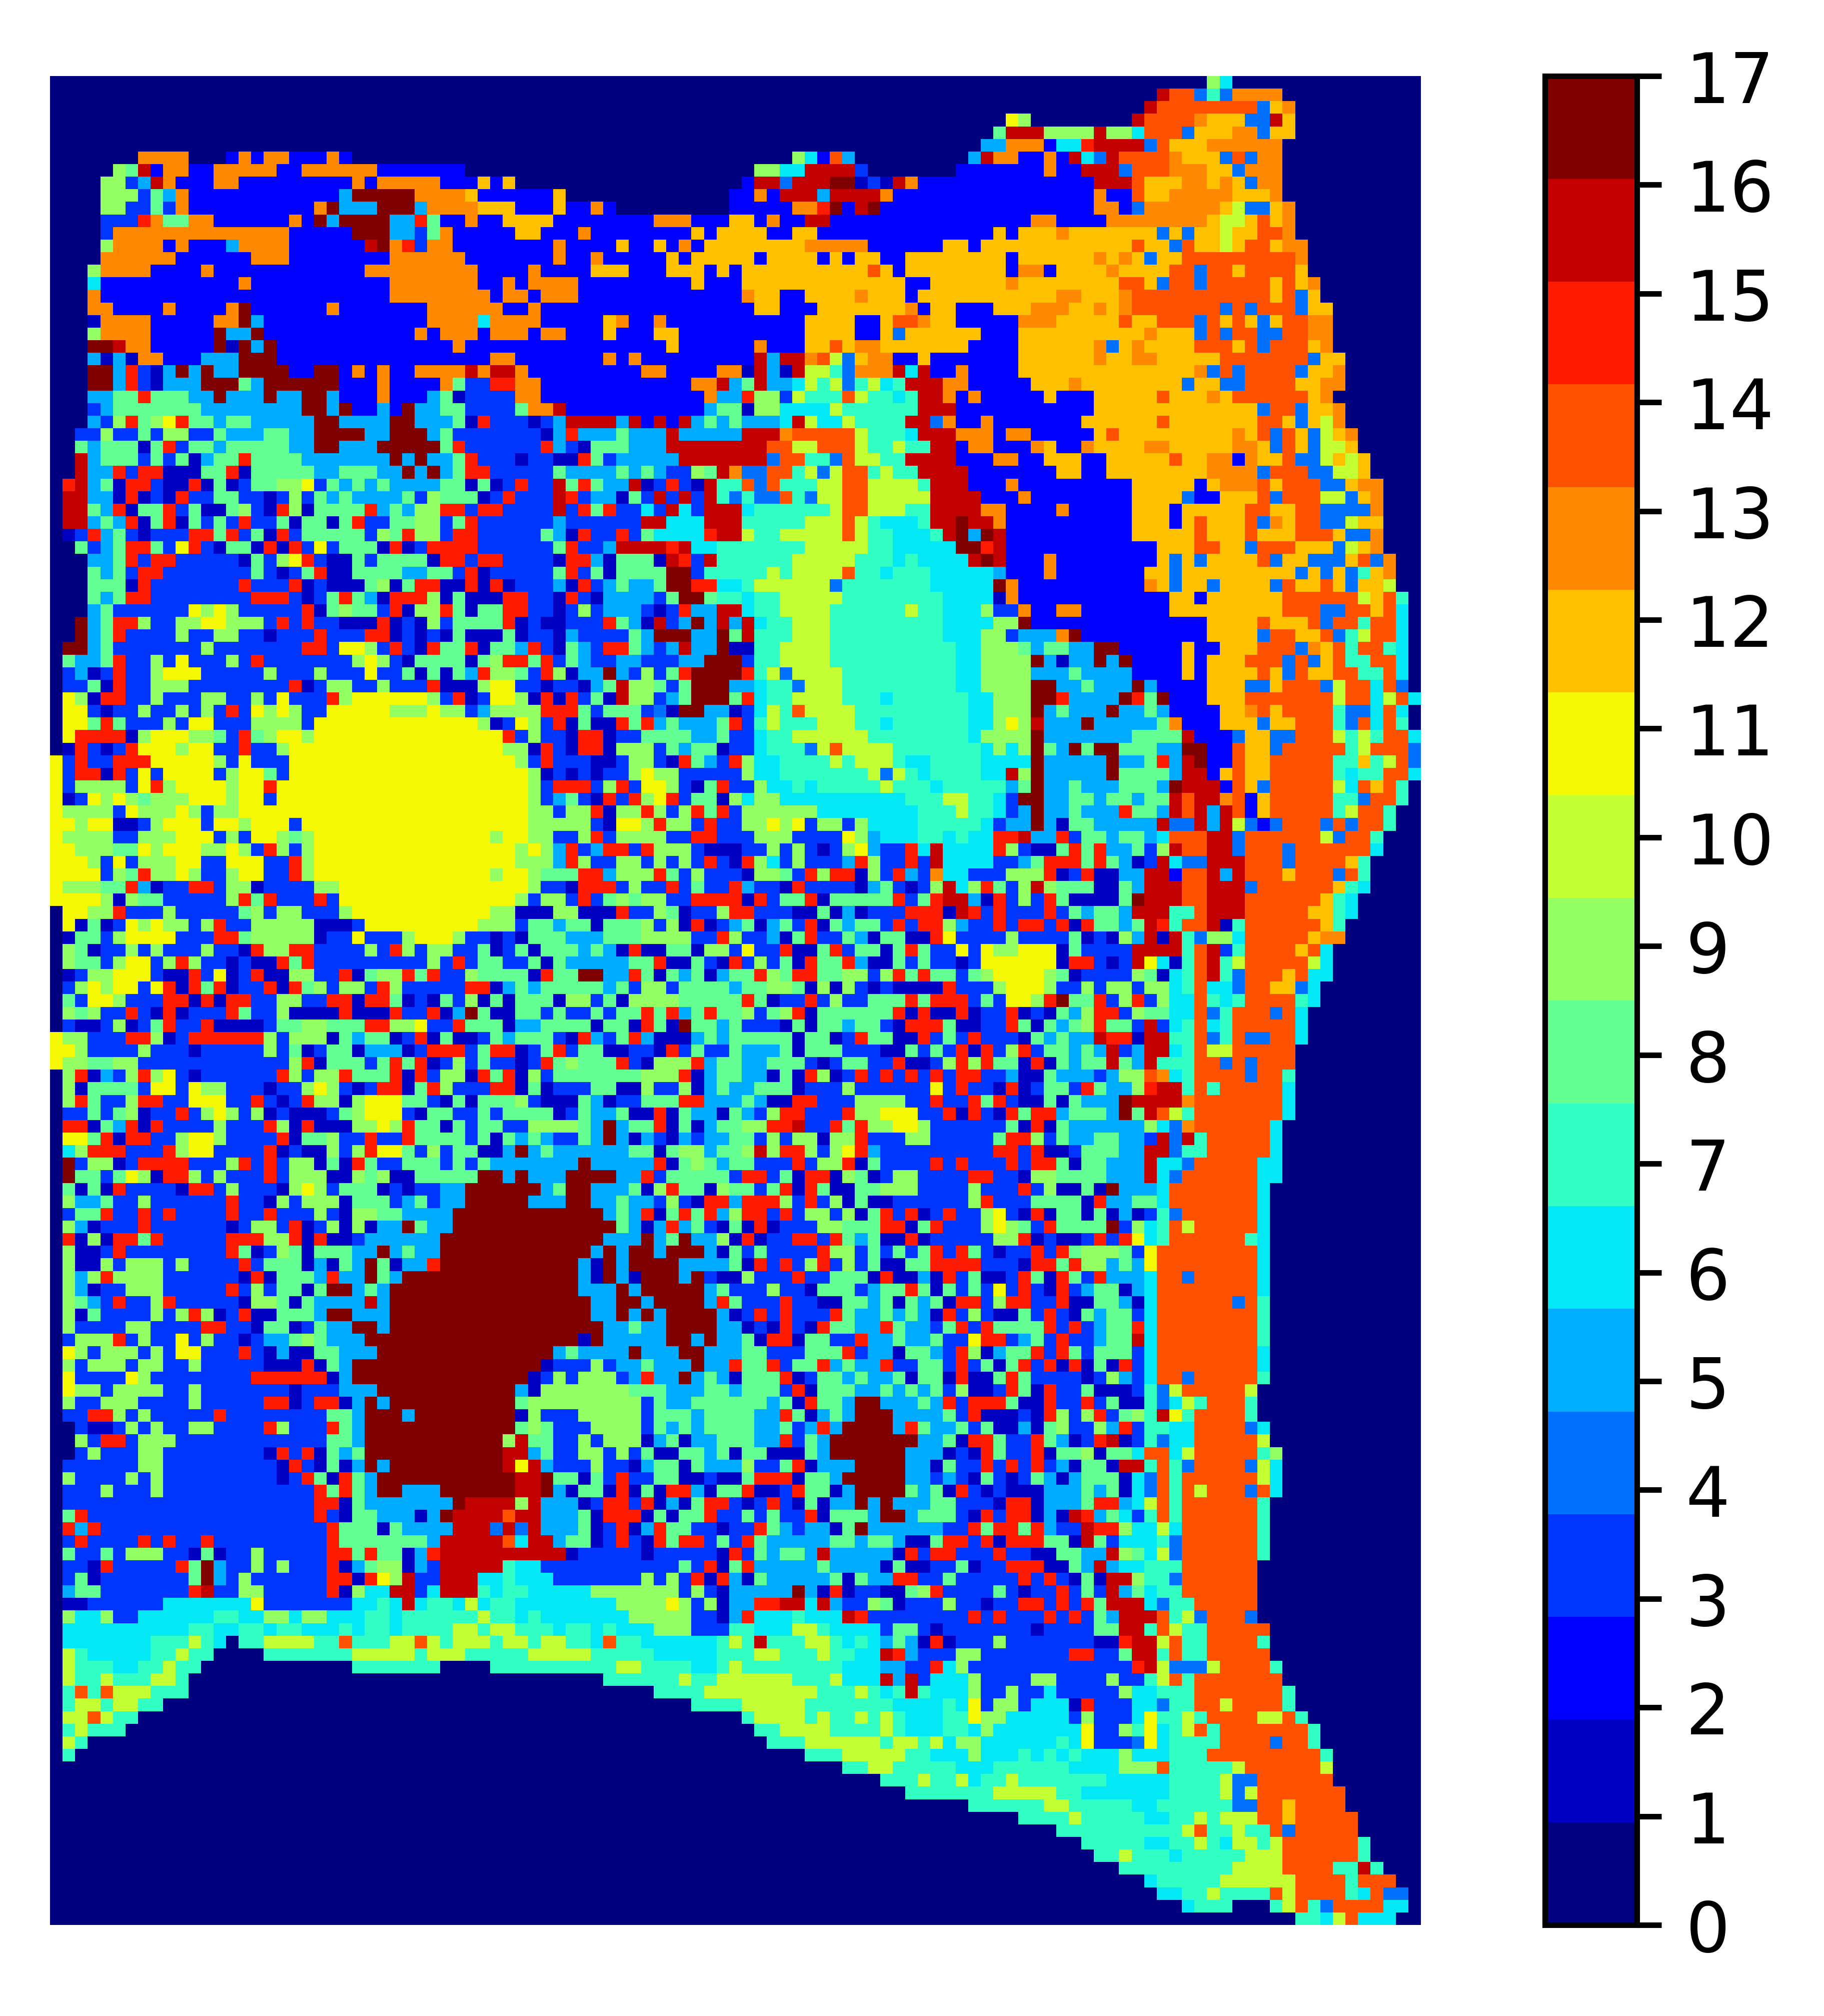
\includegraphics[width=0.3\textwidth]{pic/prostate/kmeans_all.png}
%     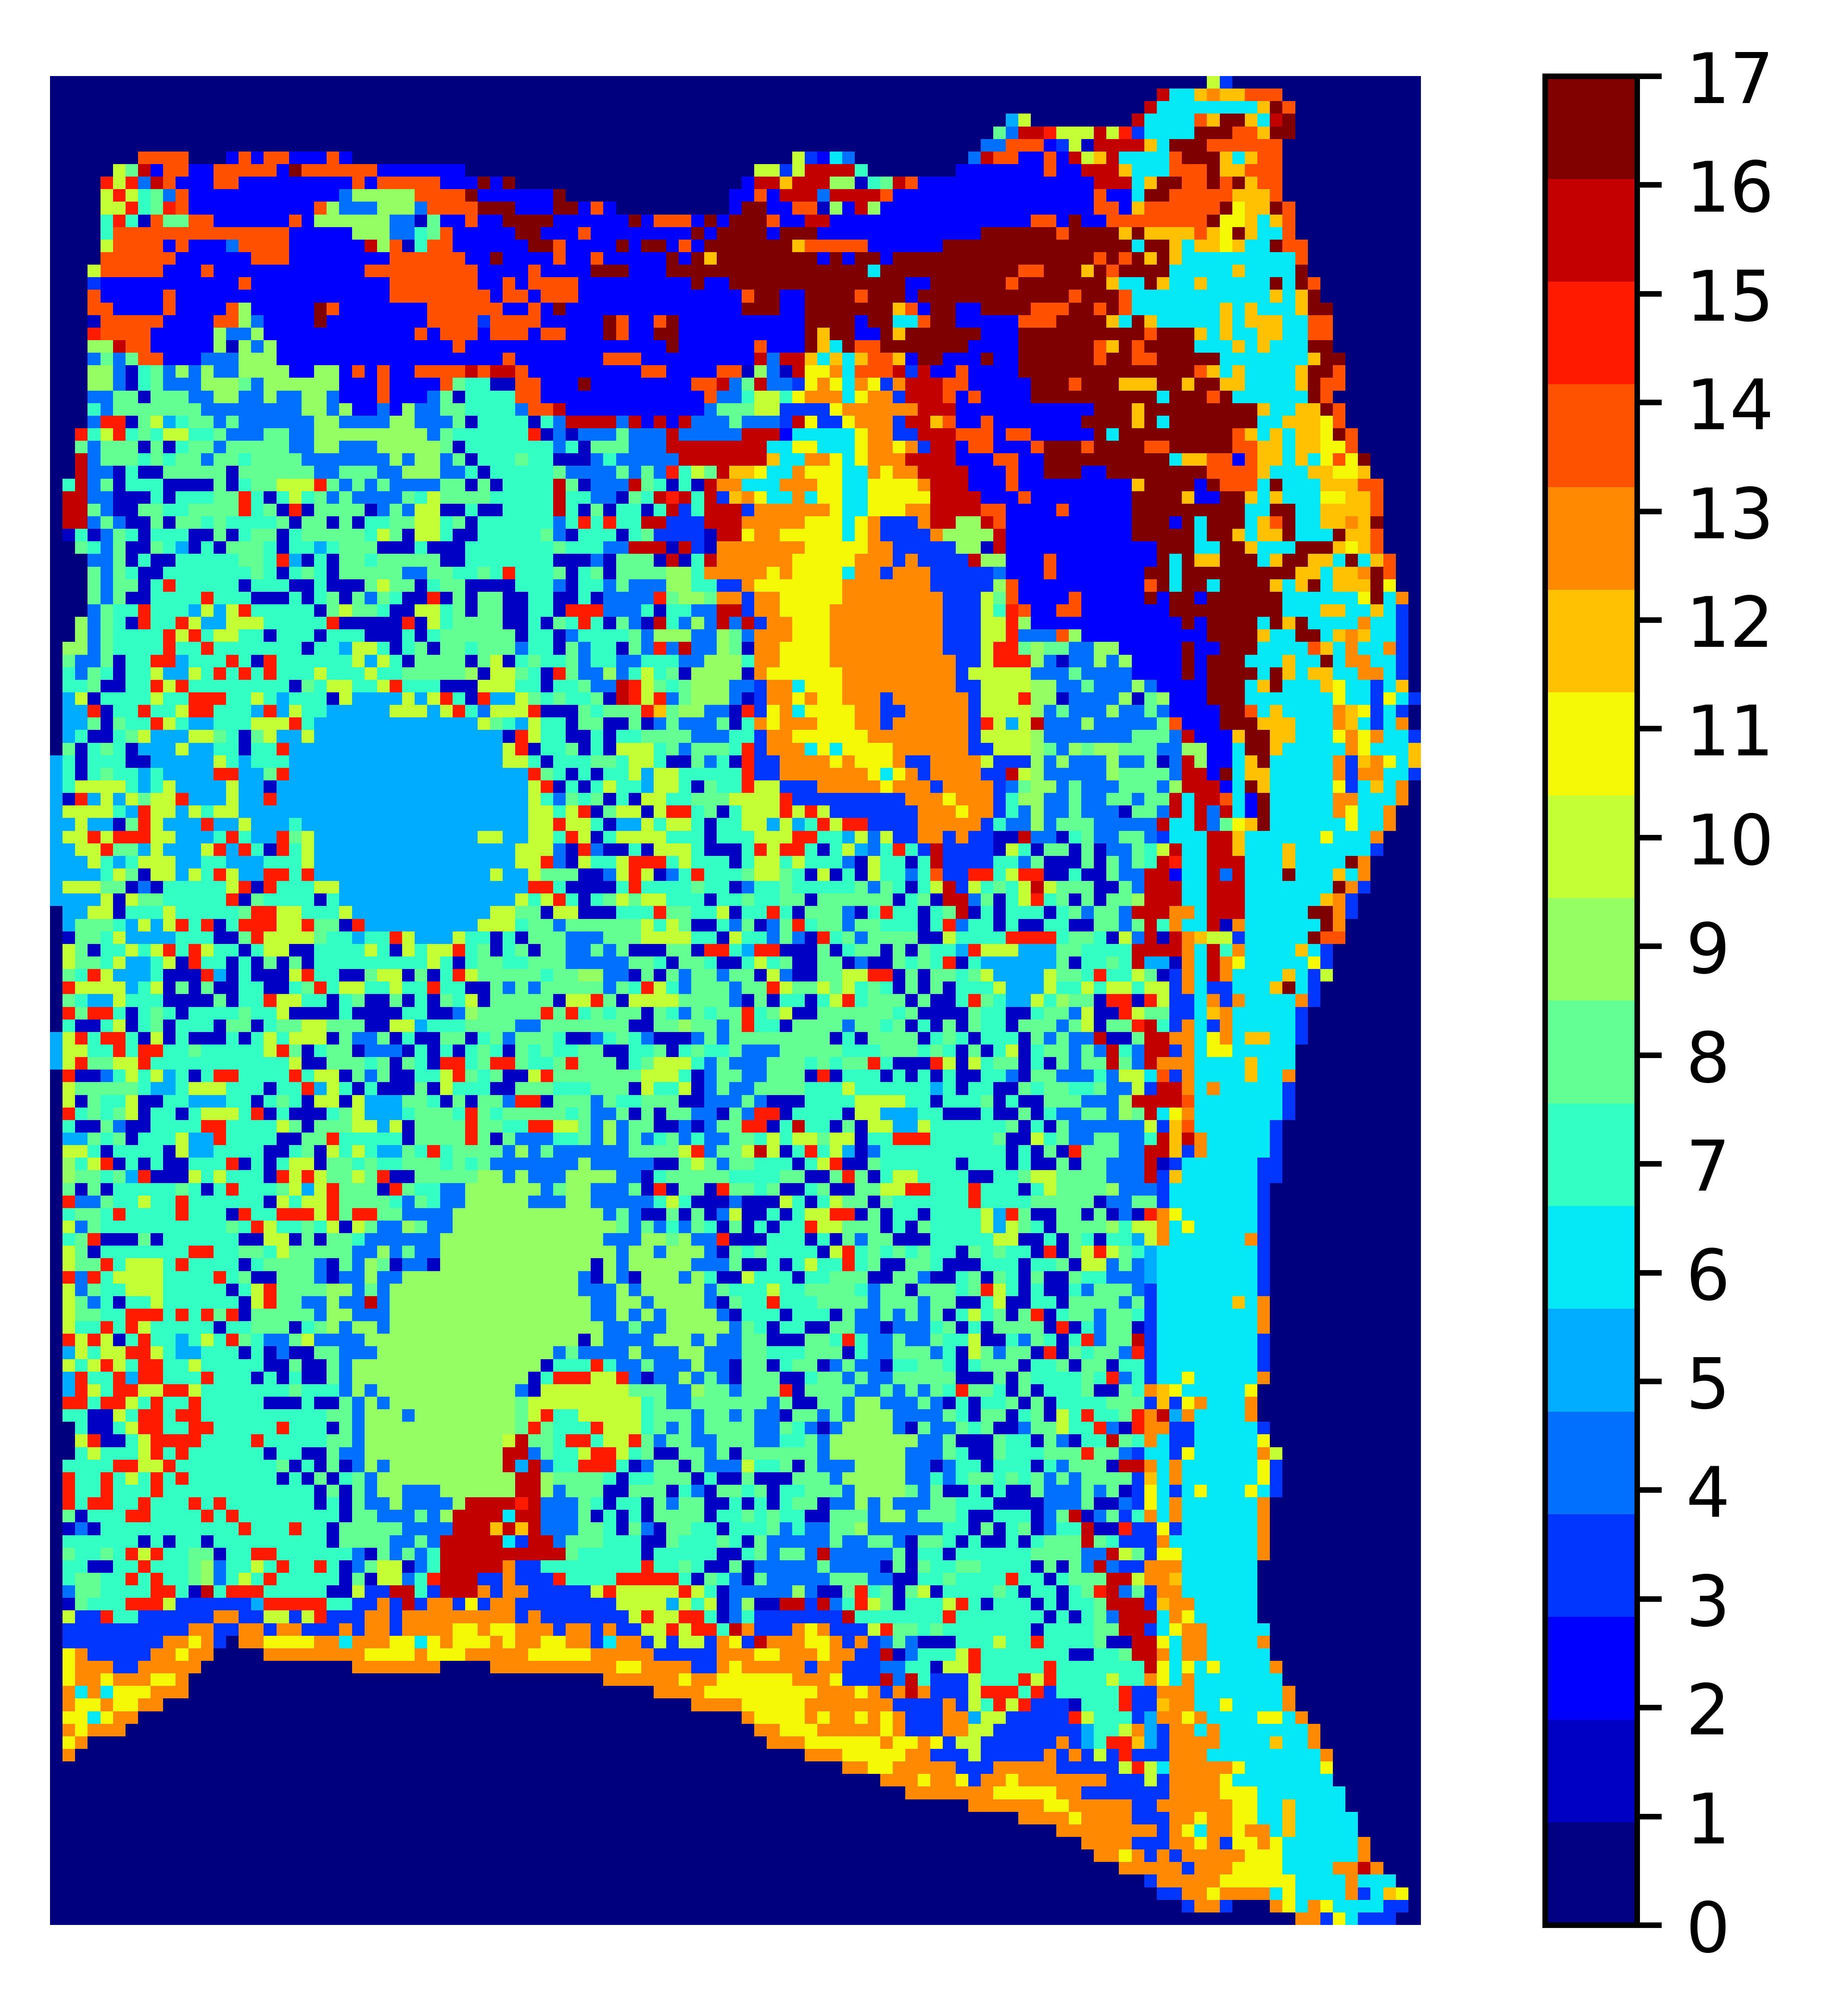
\includegraphics[width=0.3\textwidth]{pic/prostate/minibatchkmeans_all.png}
%     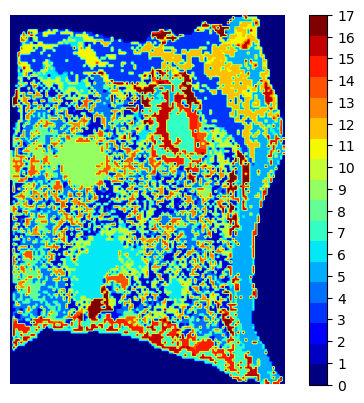
\includegraphics[width=0.3\textwidth]{pic/prostate/gmm_all.png}
%     \\
%     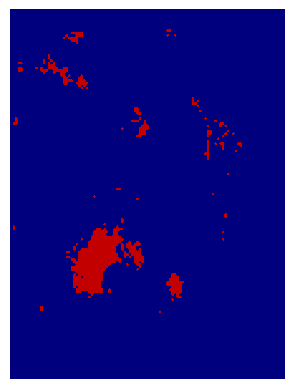
\includegraphics[width=0.3\textwidth]{pic/prostate/kmeans_selected.png}
%     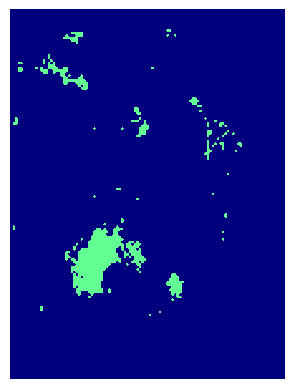
\includegraphics[width=0.3\textwidth]{pic/prostate/minibatchkmeans_selected.png}
%     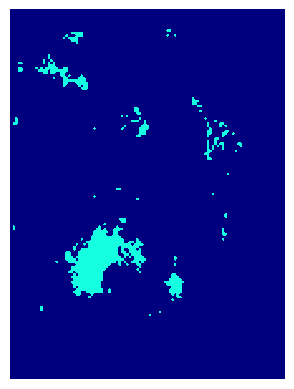
\includegraphics[width=0.3\textwidth]{pic/prostate/gmm_selected.png}
%   \captionsetup{justification=raggedright,singlelinecheck=false} 
%   \caption
%   {
%     Performance of dfifferent clustering methods on the prostate cancer dataset. 
%   }
% \end{figure}

\begin{figure}[htbp]
  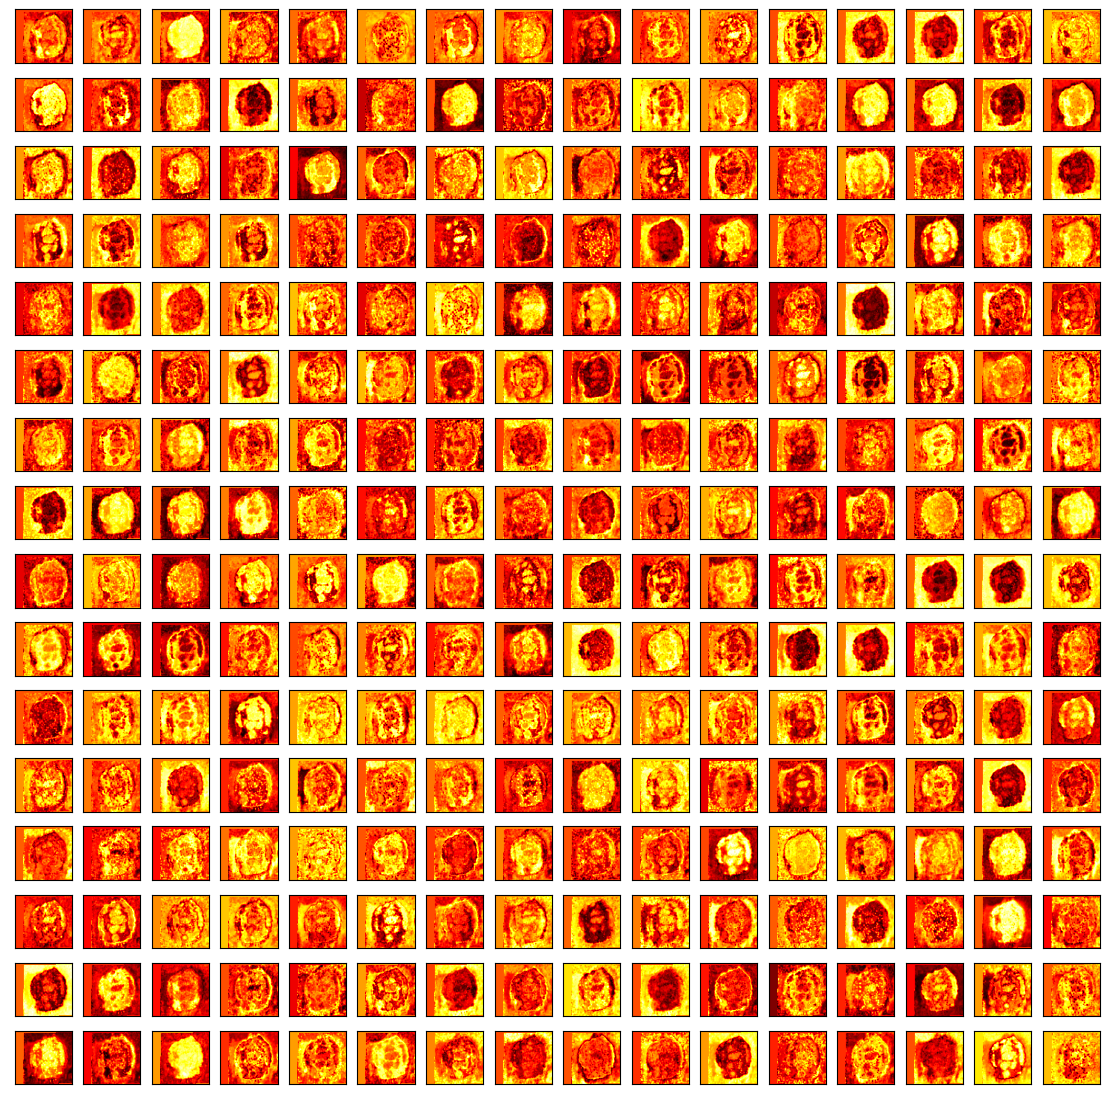
\includegraphics[width=\textwidth]{pic/encoder_feature_3D_train.png}
  \captionsetup{justification=raggedright,singlelinecheck=false}
  \caption
  {
    \textbf{Encoded features in training phase}. 
    Low-dimensional encoded features 
    efficiently capture molecular structures 
    from original high-dimensional data. 
  }
  \label{fig:encoder_feature_3D_train}
\end{figure}
\begin{figure}[htbp]
    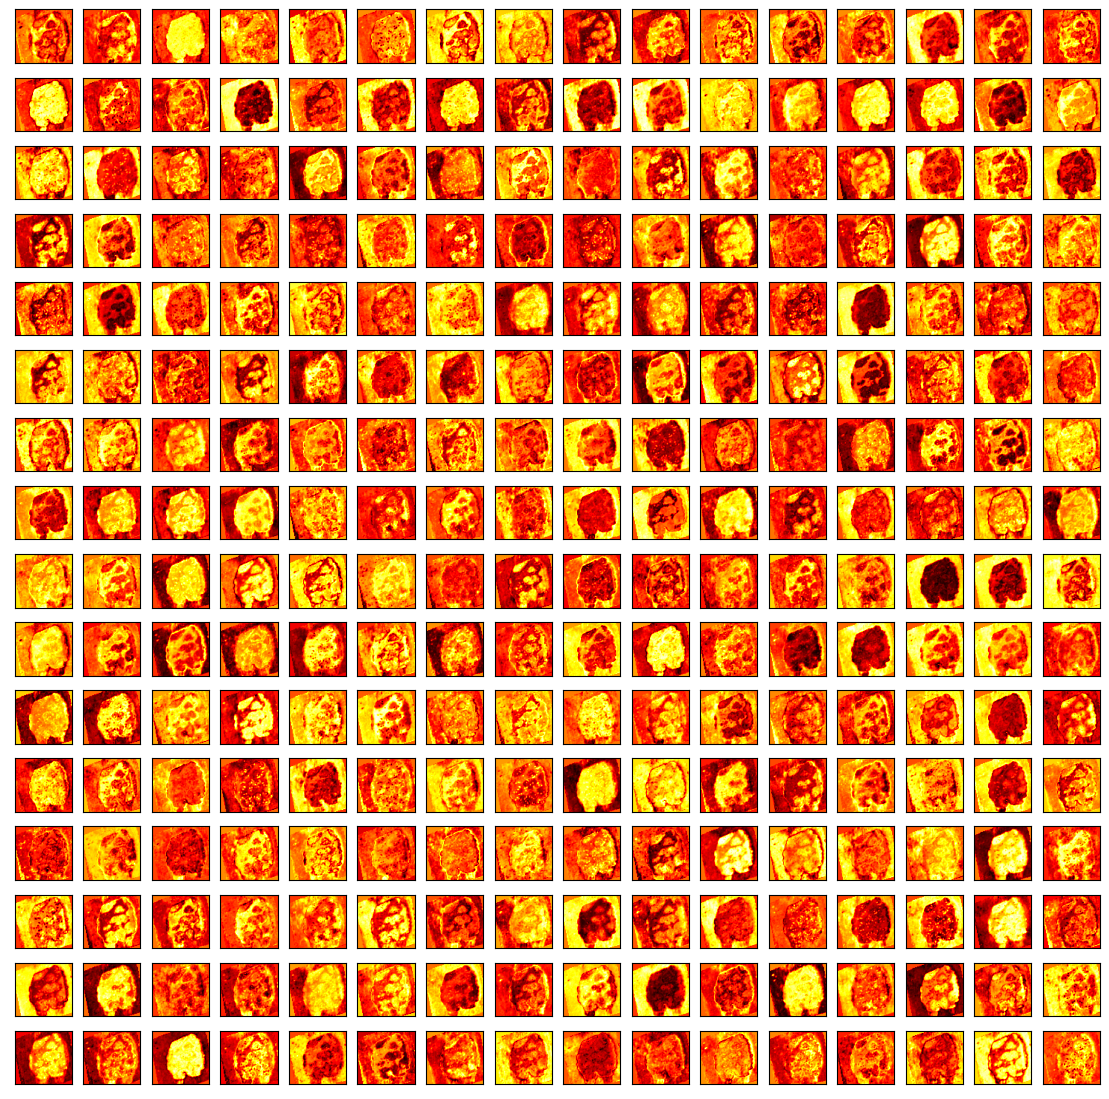
\includegraphics[width=\linewidth]{pic/encoder_feature_3D_test.png}
    \captionsetup{justification=raggedright,singlelinecheck=false}
    \caption
    {
      \textbf{Encoded features in testing phase}. 
      Similar to the encoding features generated during the 
      training process, the 256-dimensional features effectively 
      integrate the nonlinear manifold within the raw data, yielding 
      comparable outcomes. This similarity underscores 
      the absence of significant overfitting in the model. 
    }
    \label{fig:encoder_feature_3D_test}
\end{figure}


\newpage

\begin{figure}[htbp]
  \centering
  % \begin{minipage}[c]{0.9\textwidth}
  % {
  %   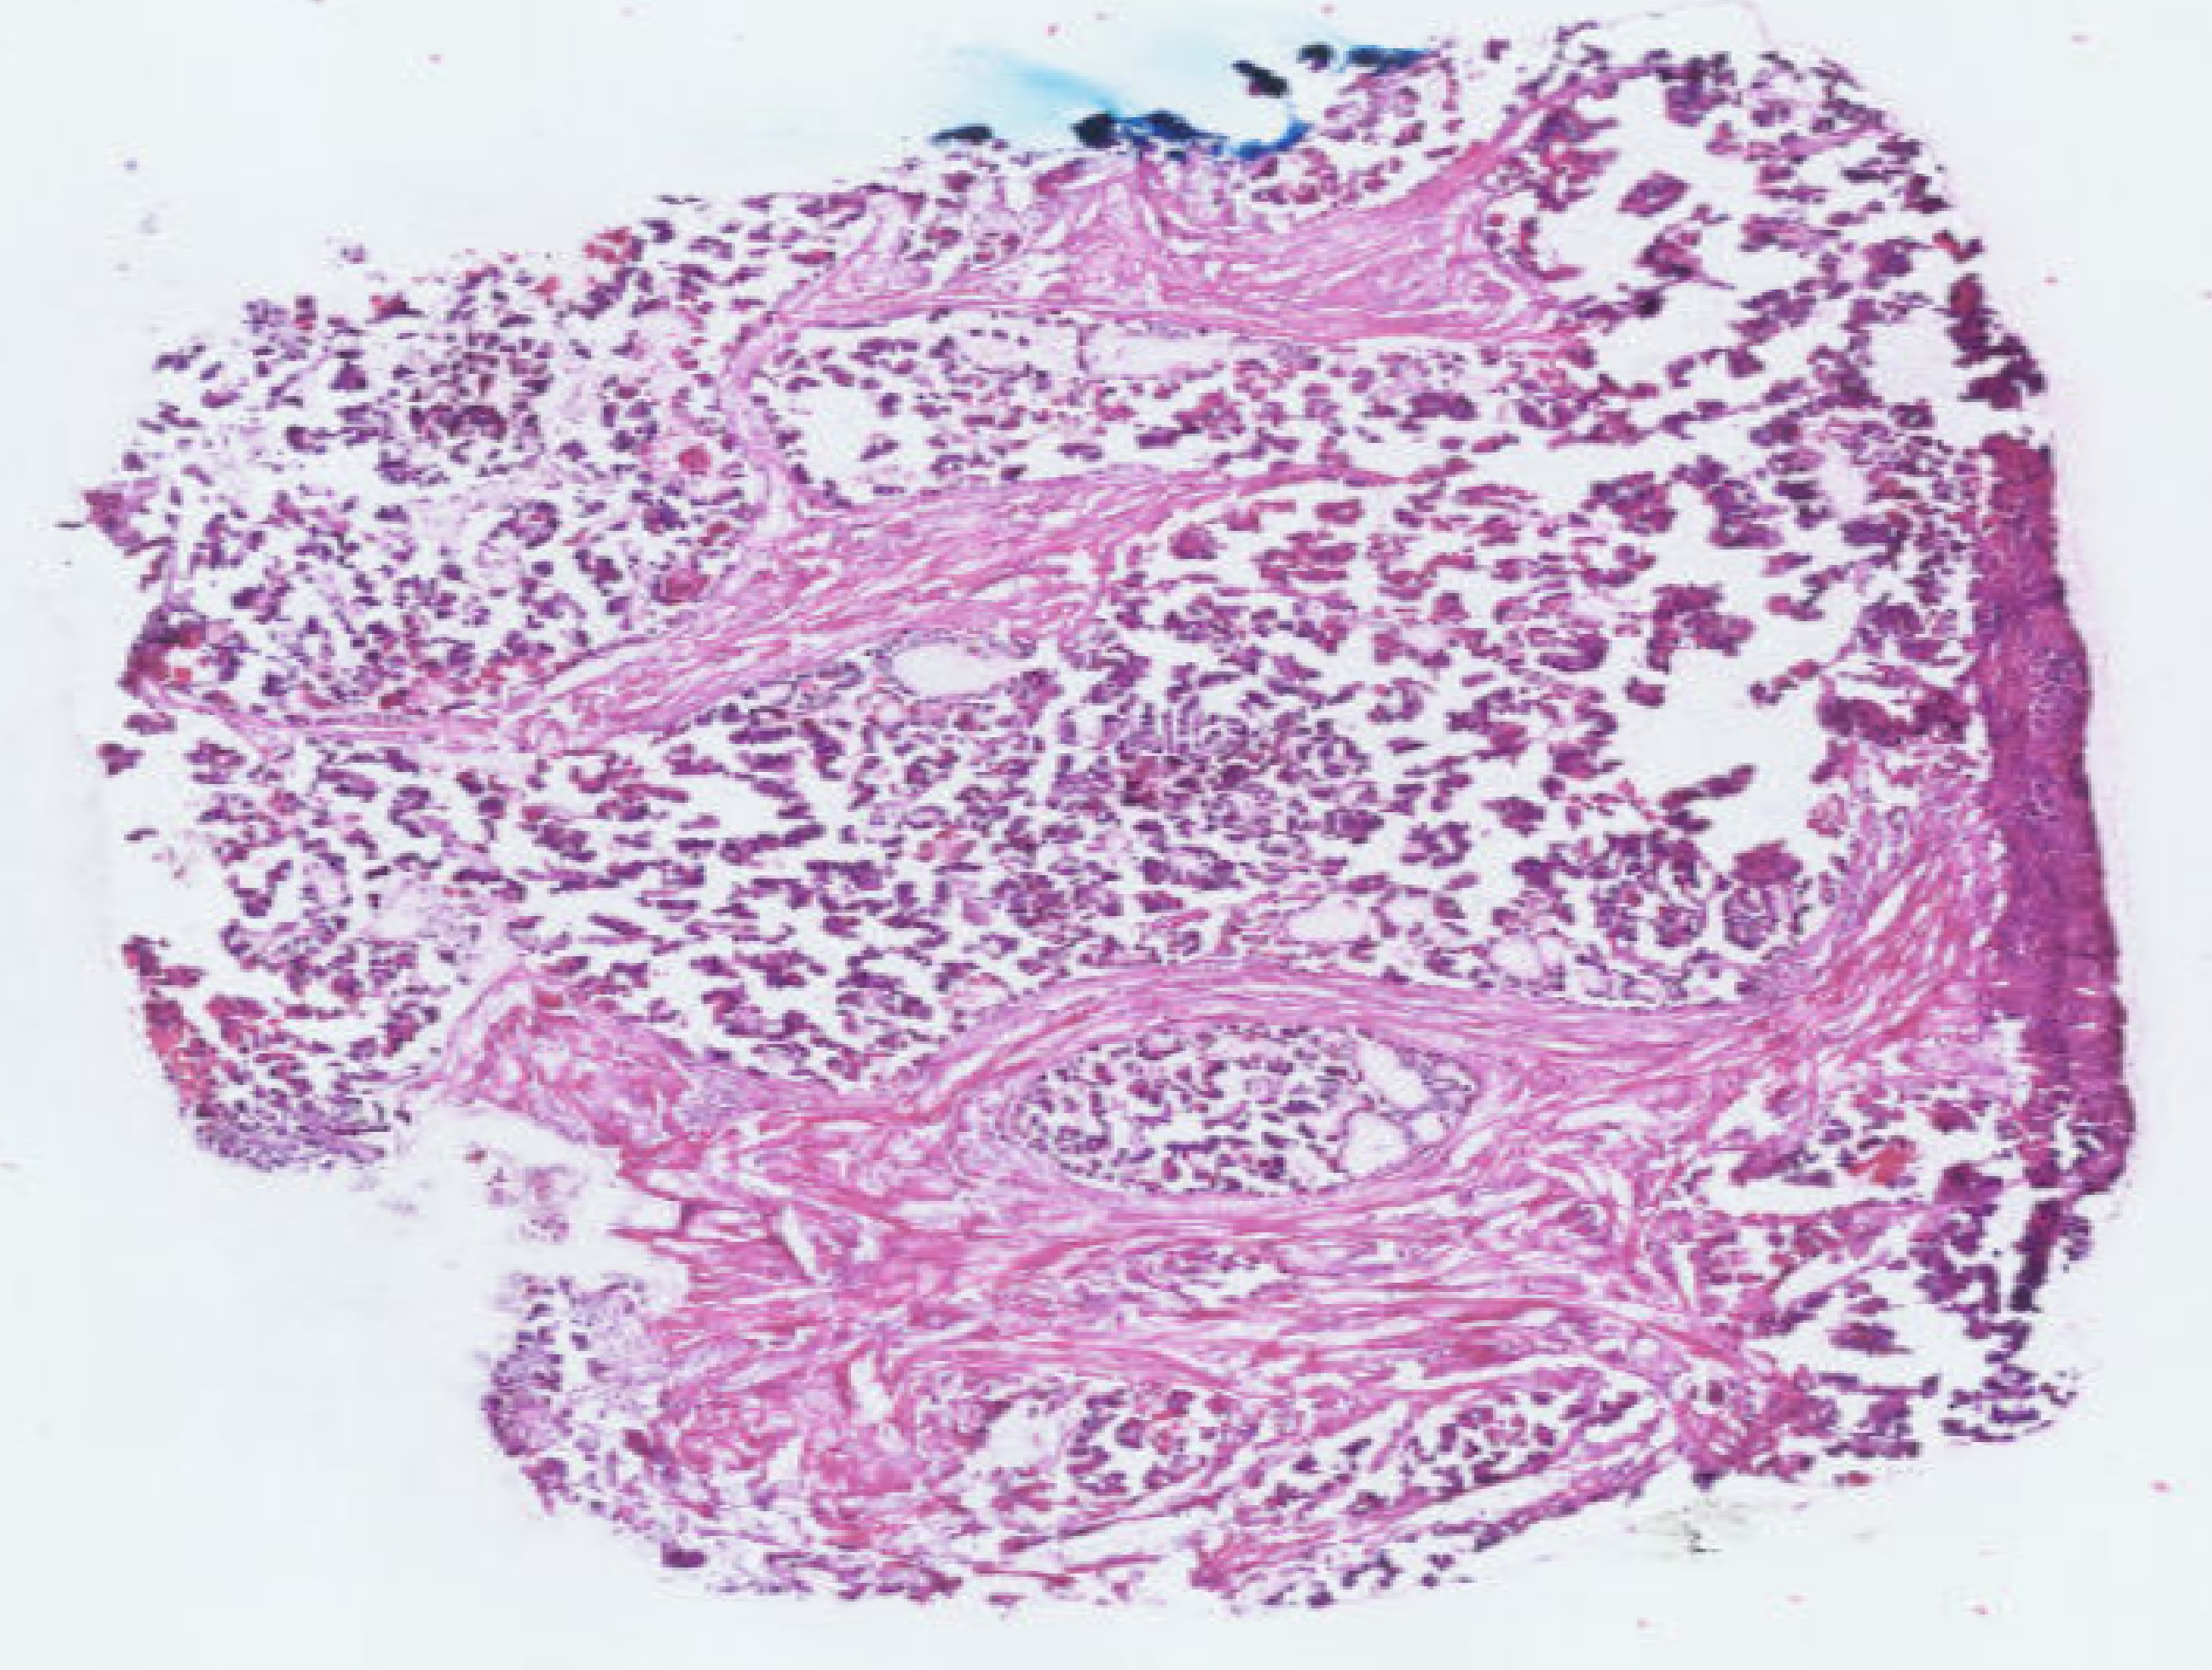
\includegraphics[width=\colWidth\textwidth]{pic/colorectal/s1_op.png}
  %   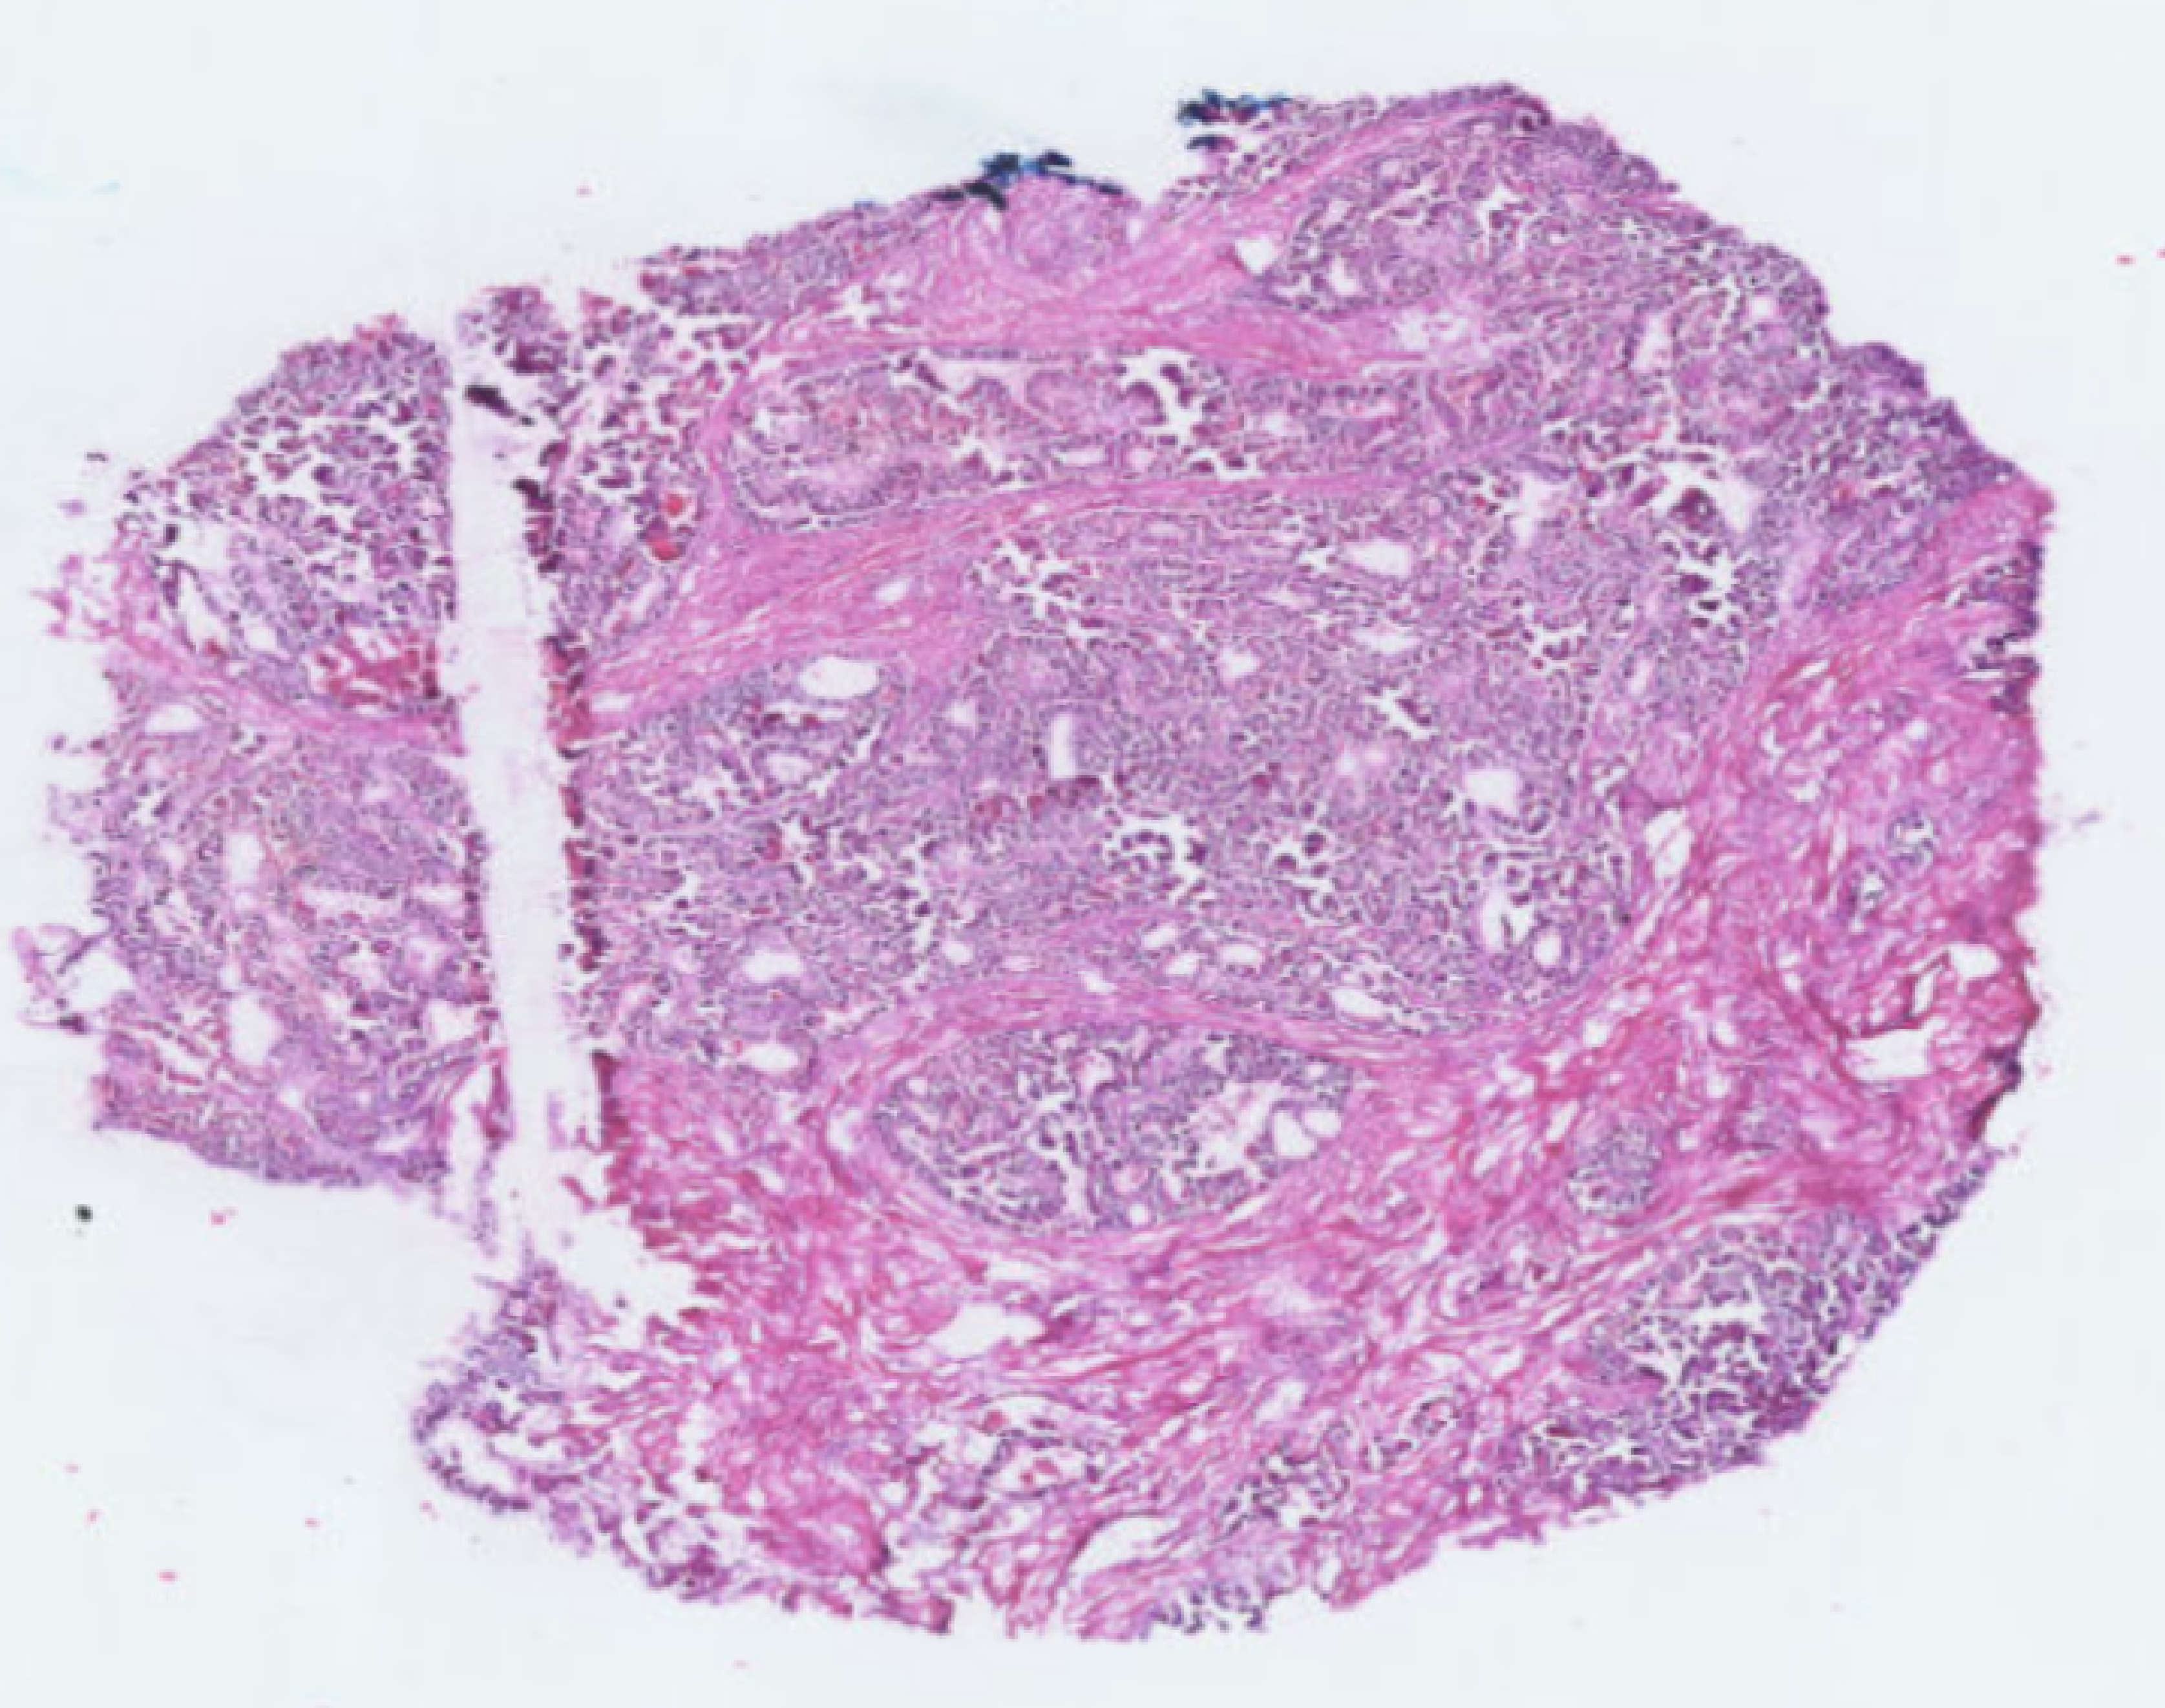
\includegraphics[width=\colWidth\textwidth]{pic/colorectal/s2_op.png}
  %   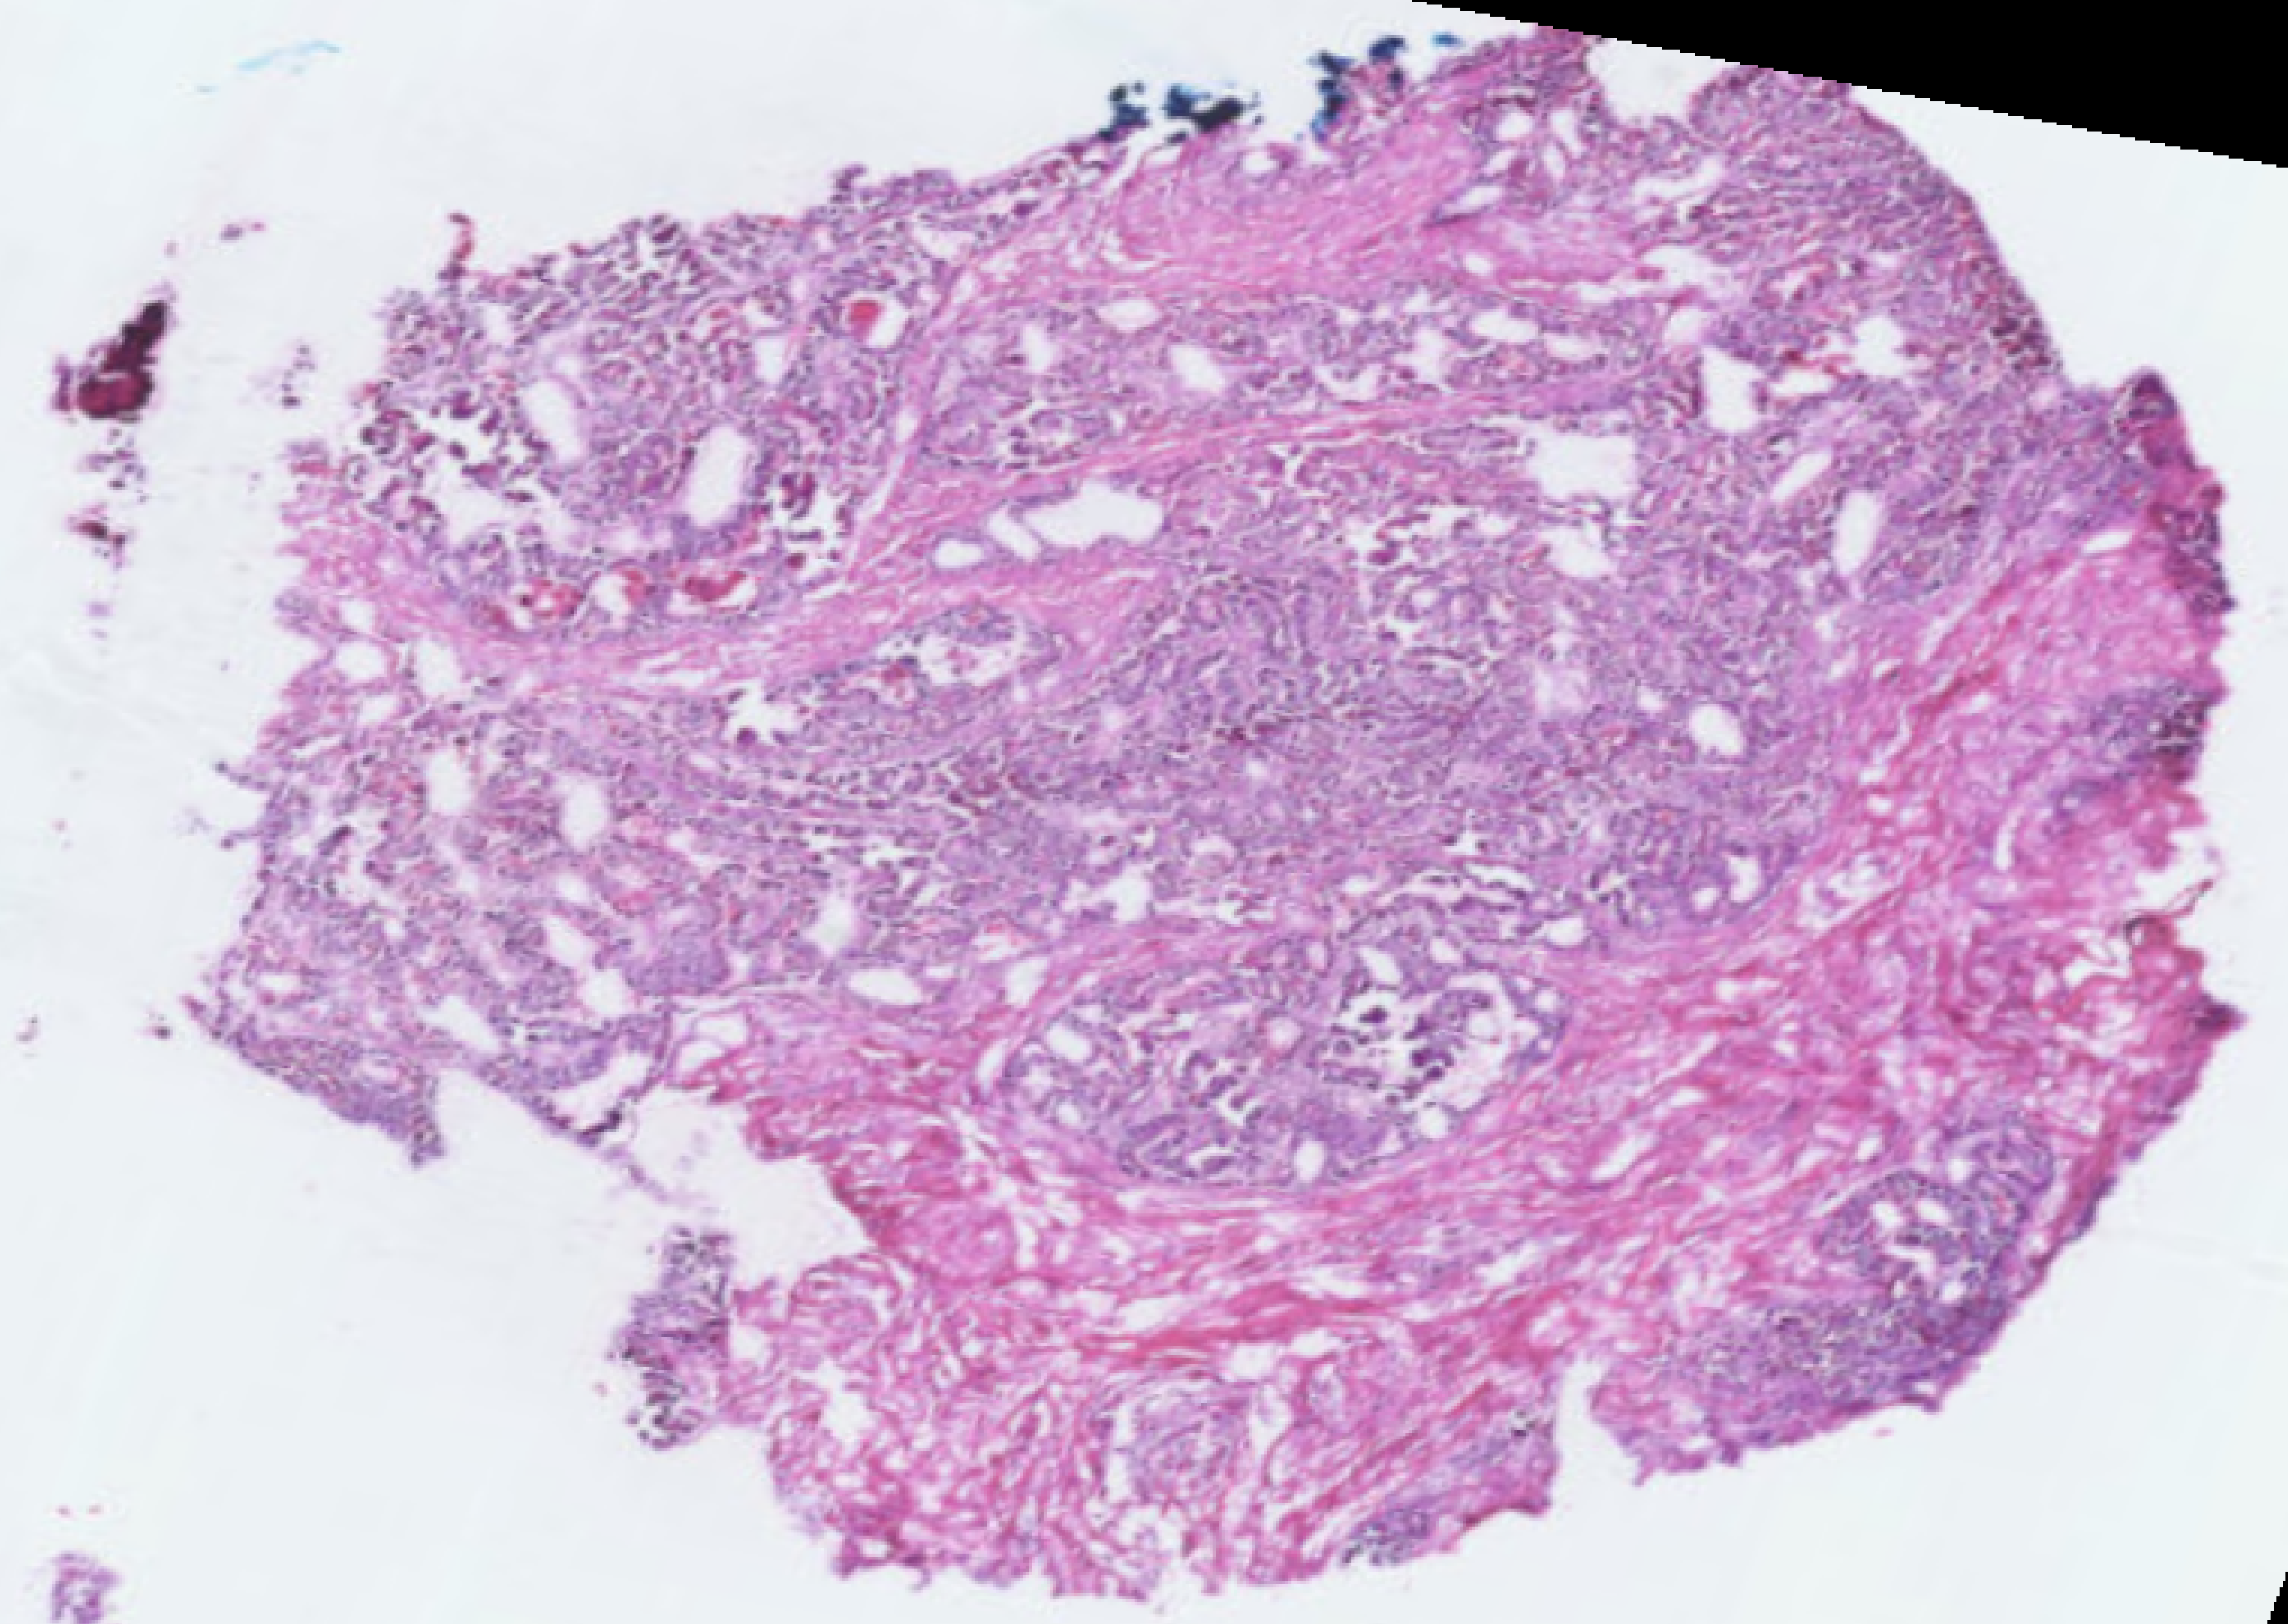
\includegraphics[width=\colWidth\textwidth]{pic/colorectal/s3_op.png}
  %   \includegraphics[width=\colWidth\textwidth]{pic/colorectal/s4_op.png}
  %   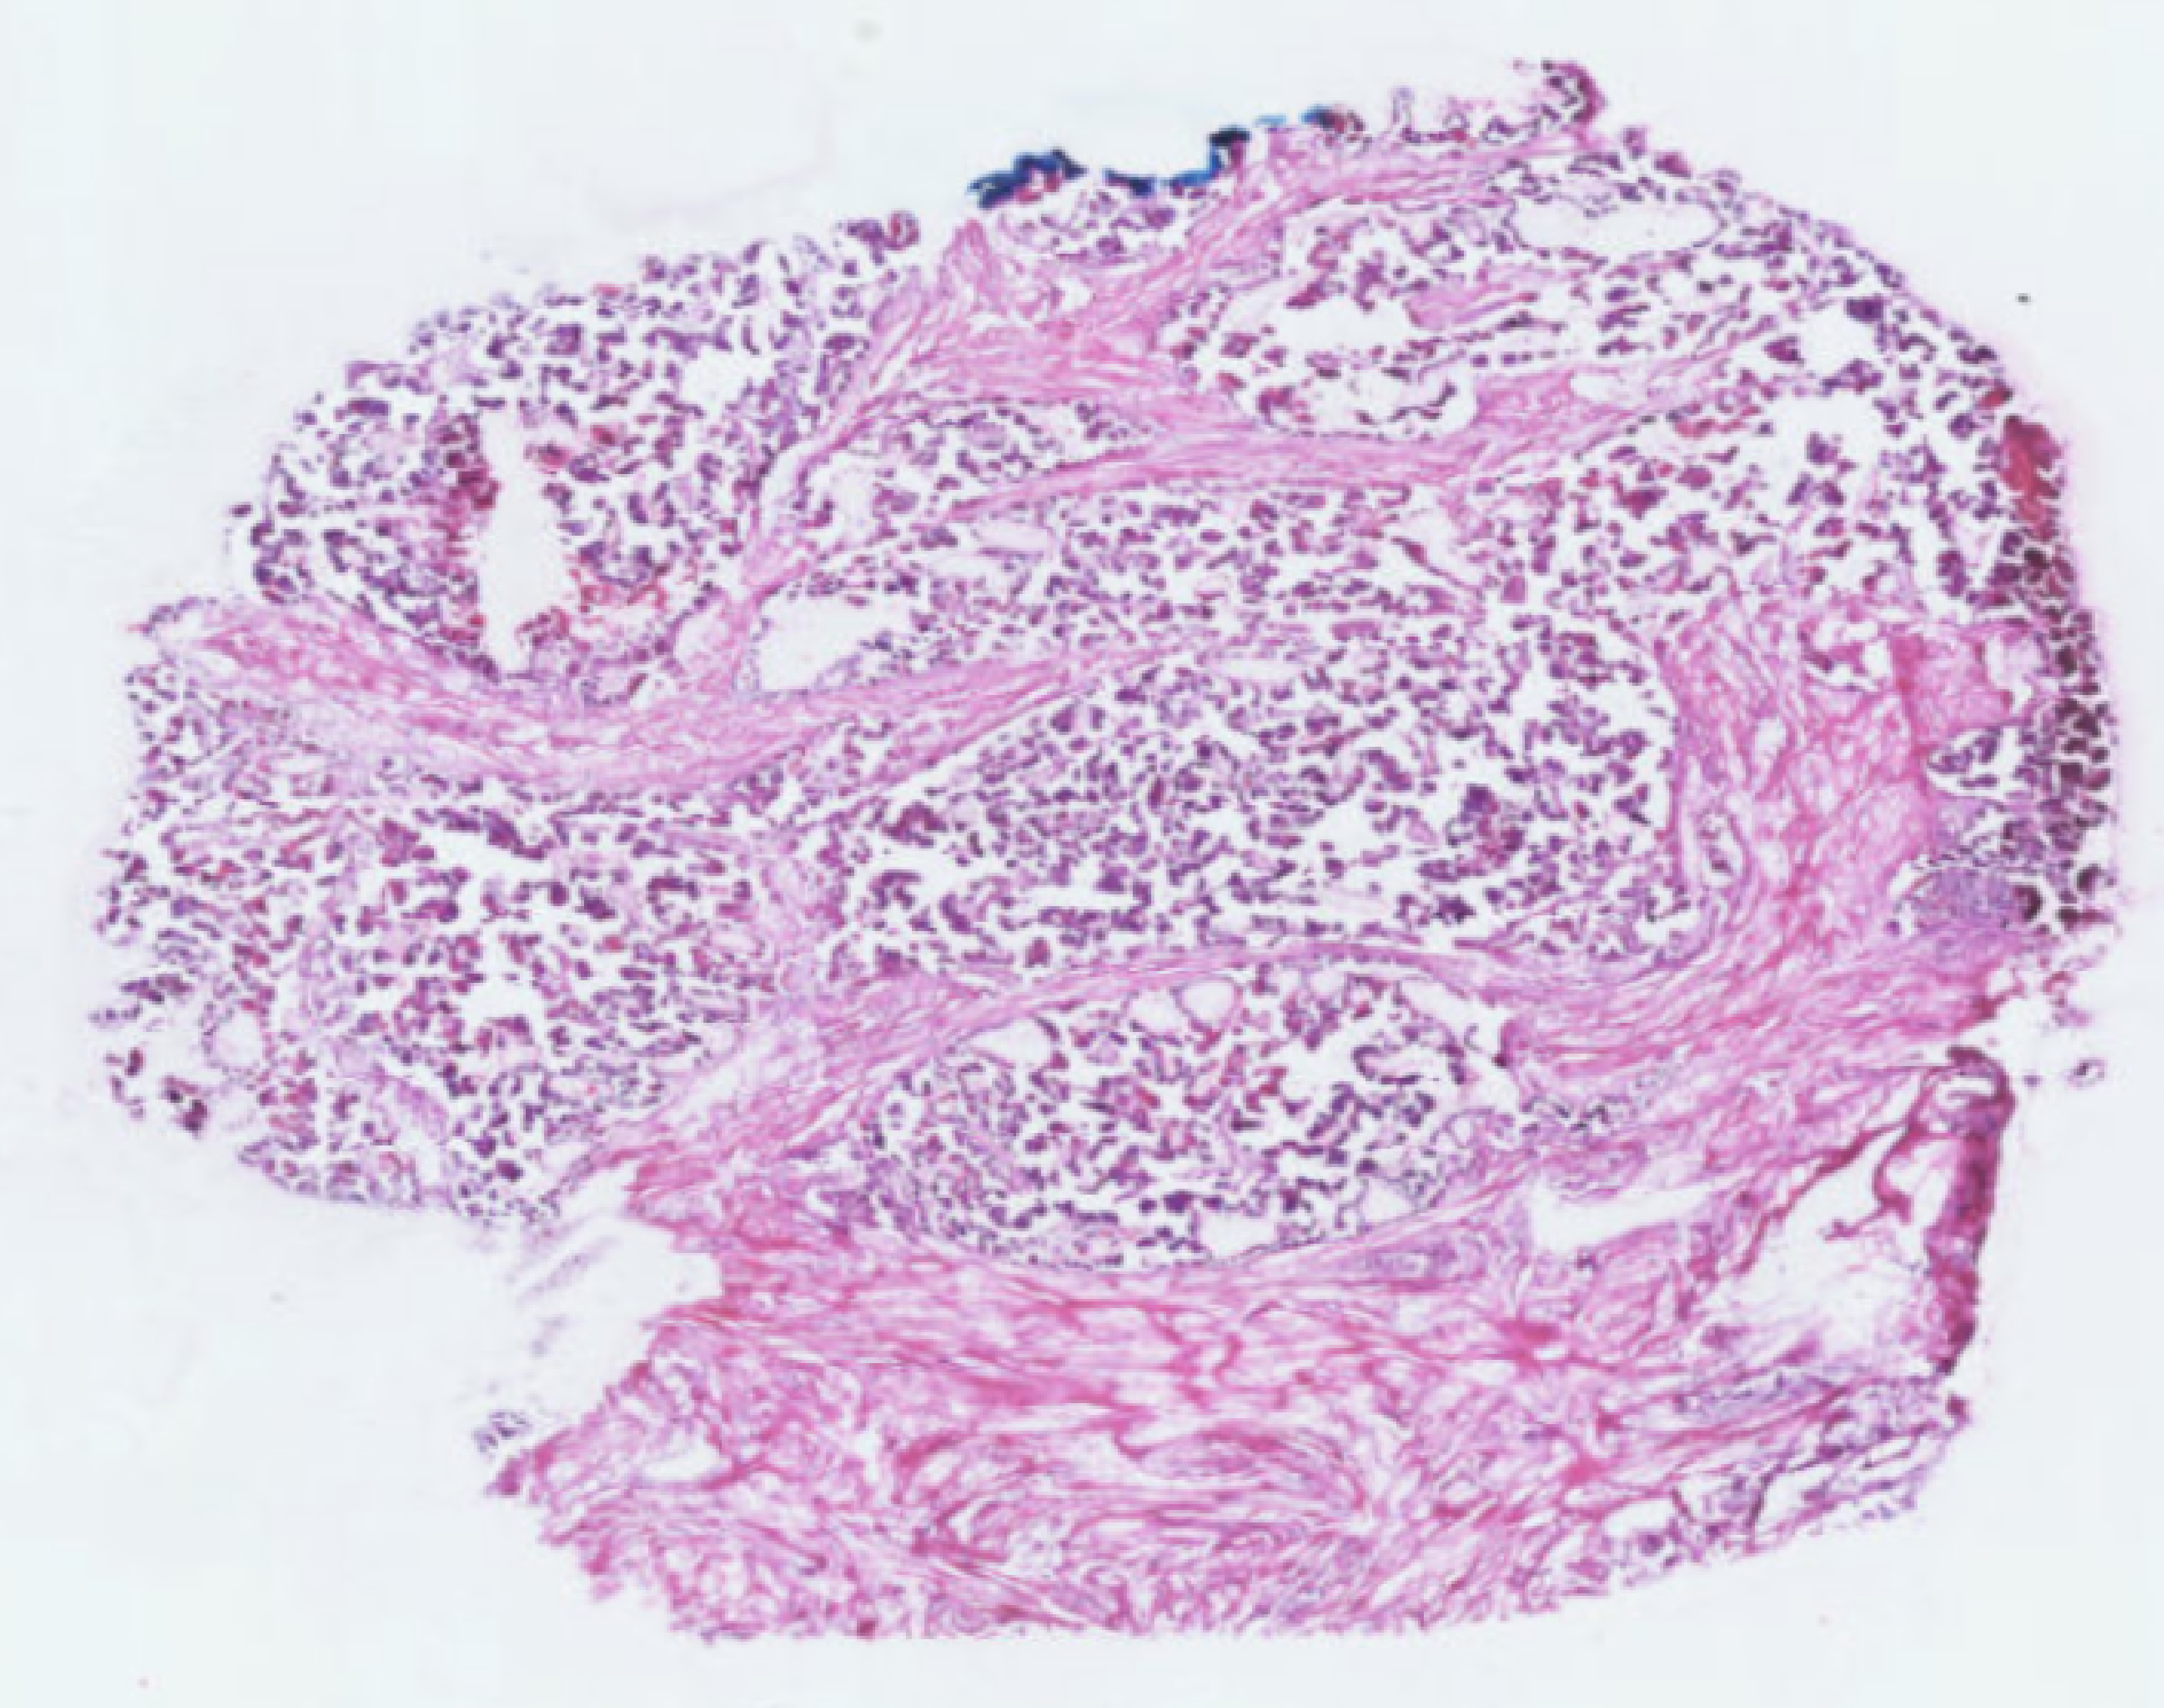
\includegraphics[width=\colWidth\textwidth]{pic/colorectal/s5_op.png}
  %   \\
  %   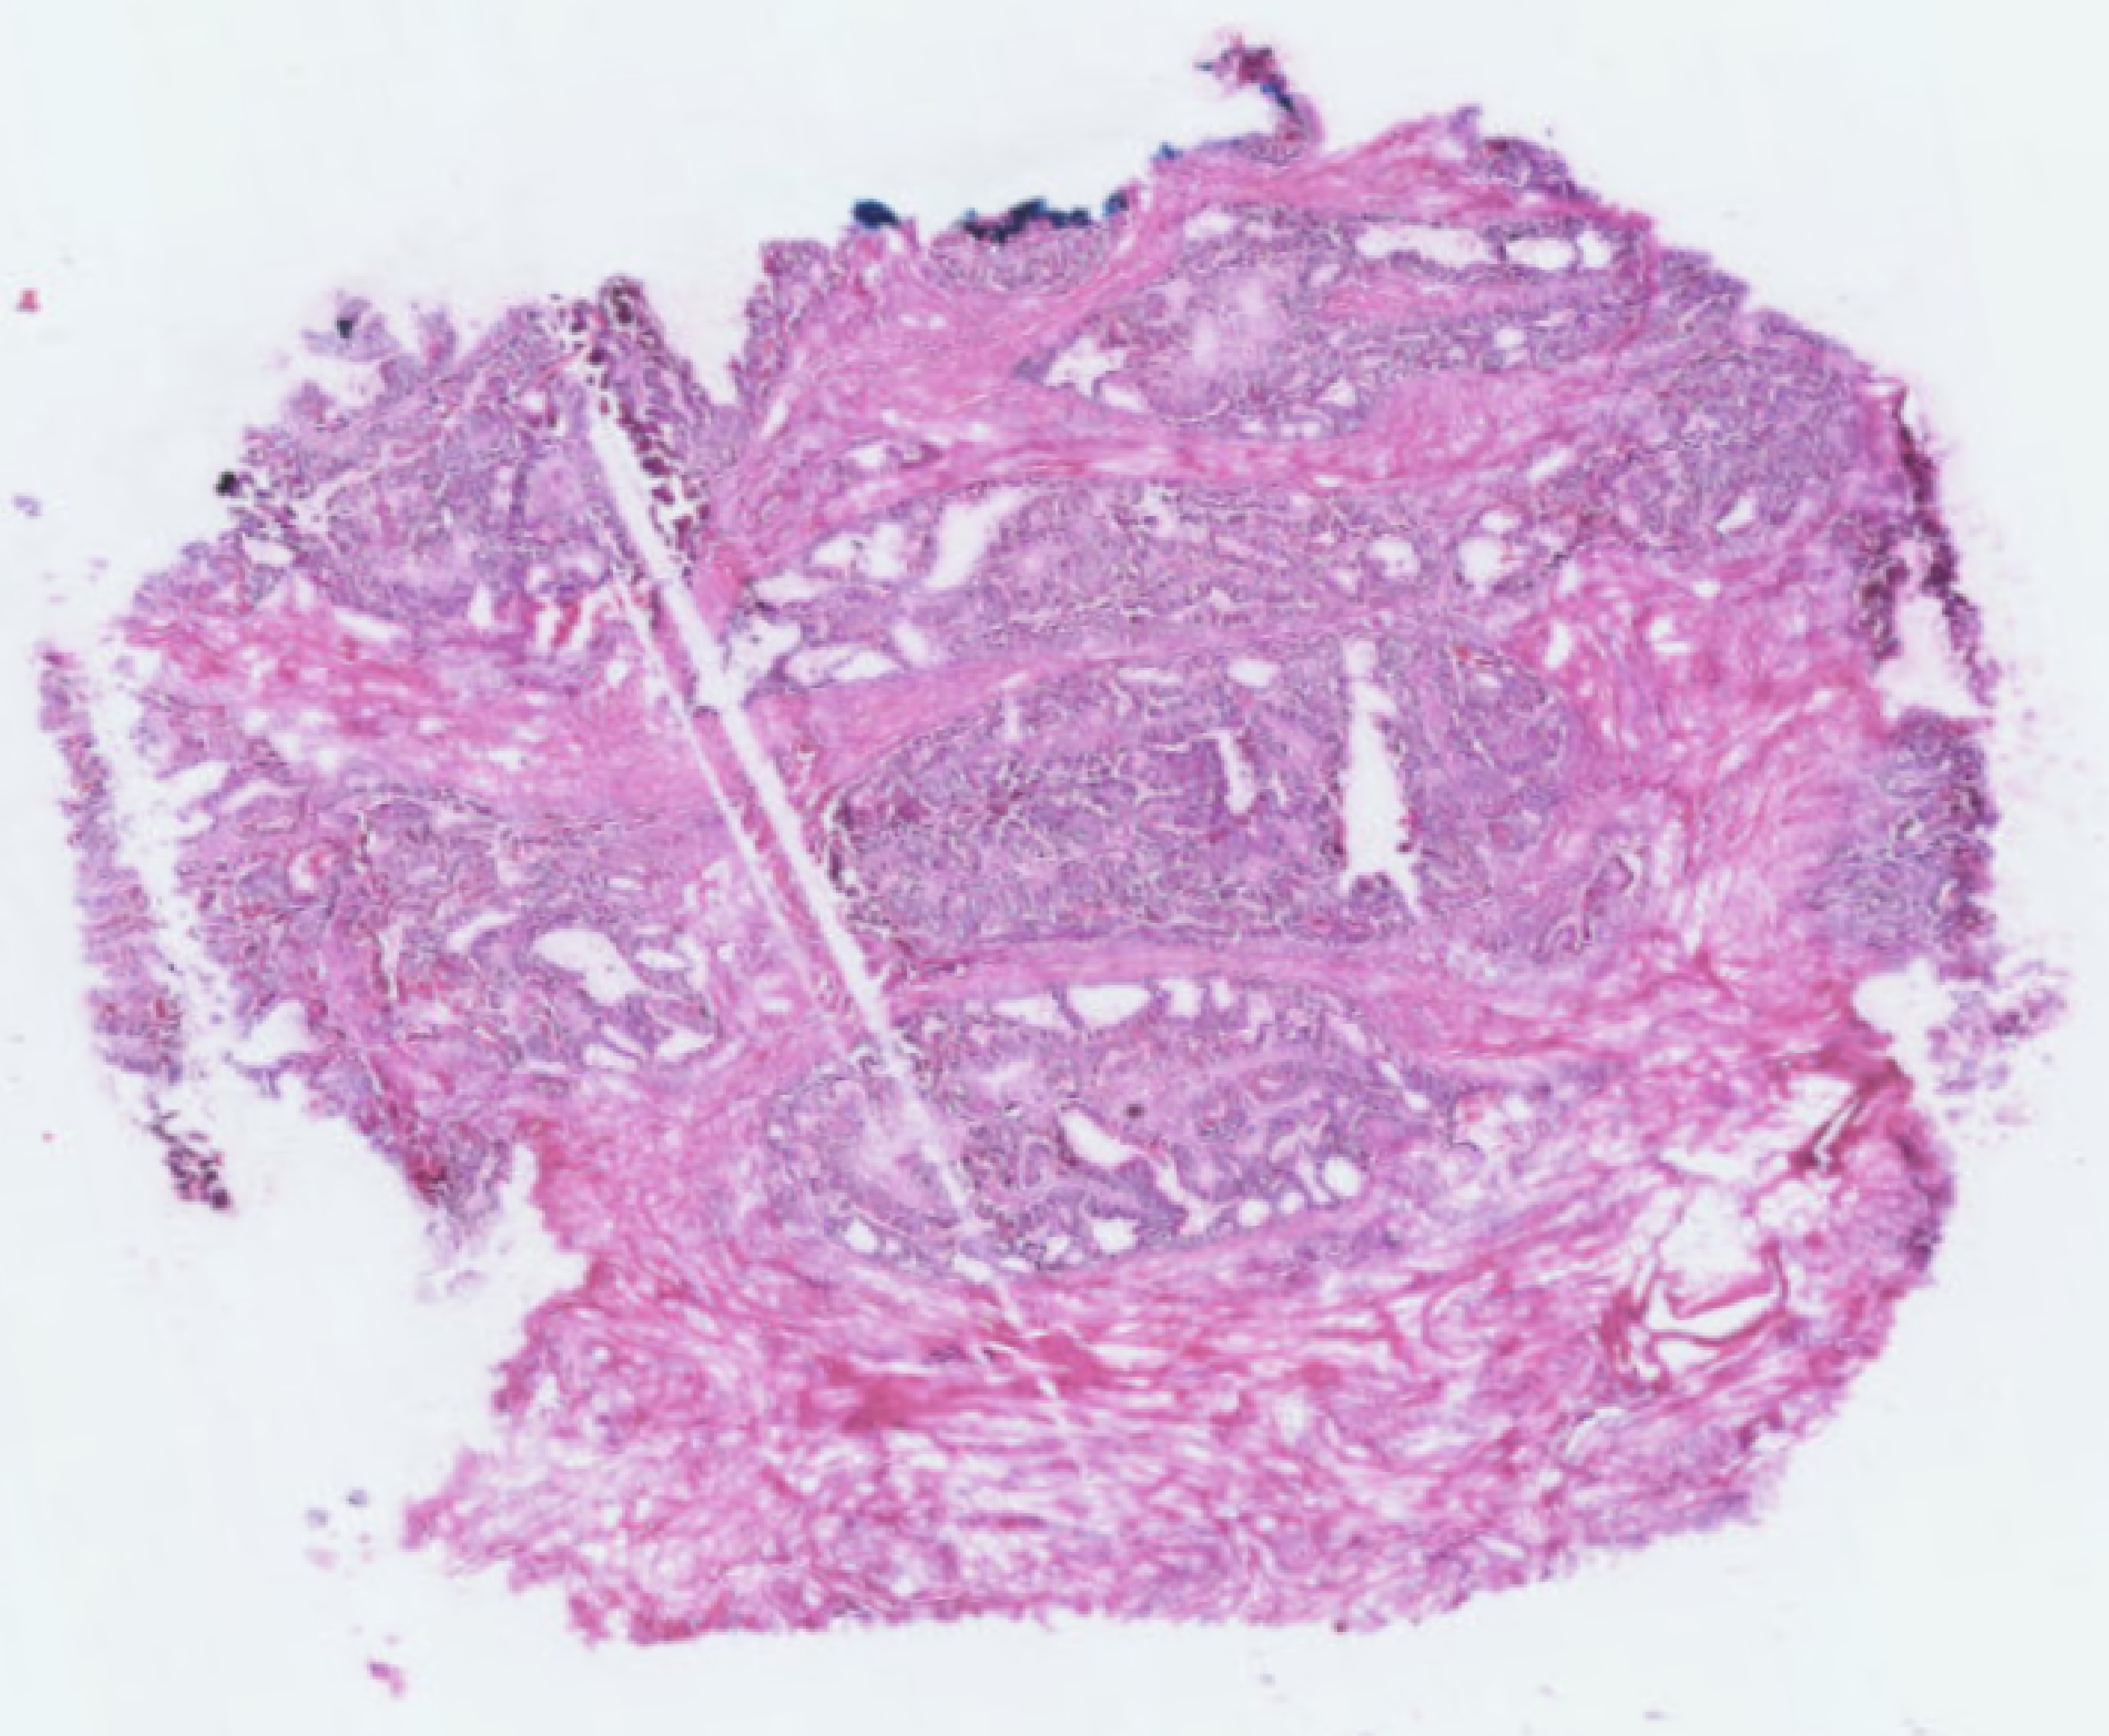
\includegraphics[width=\colWidth\textwidth]{pic/colorectal/s6_op.png}
  %   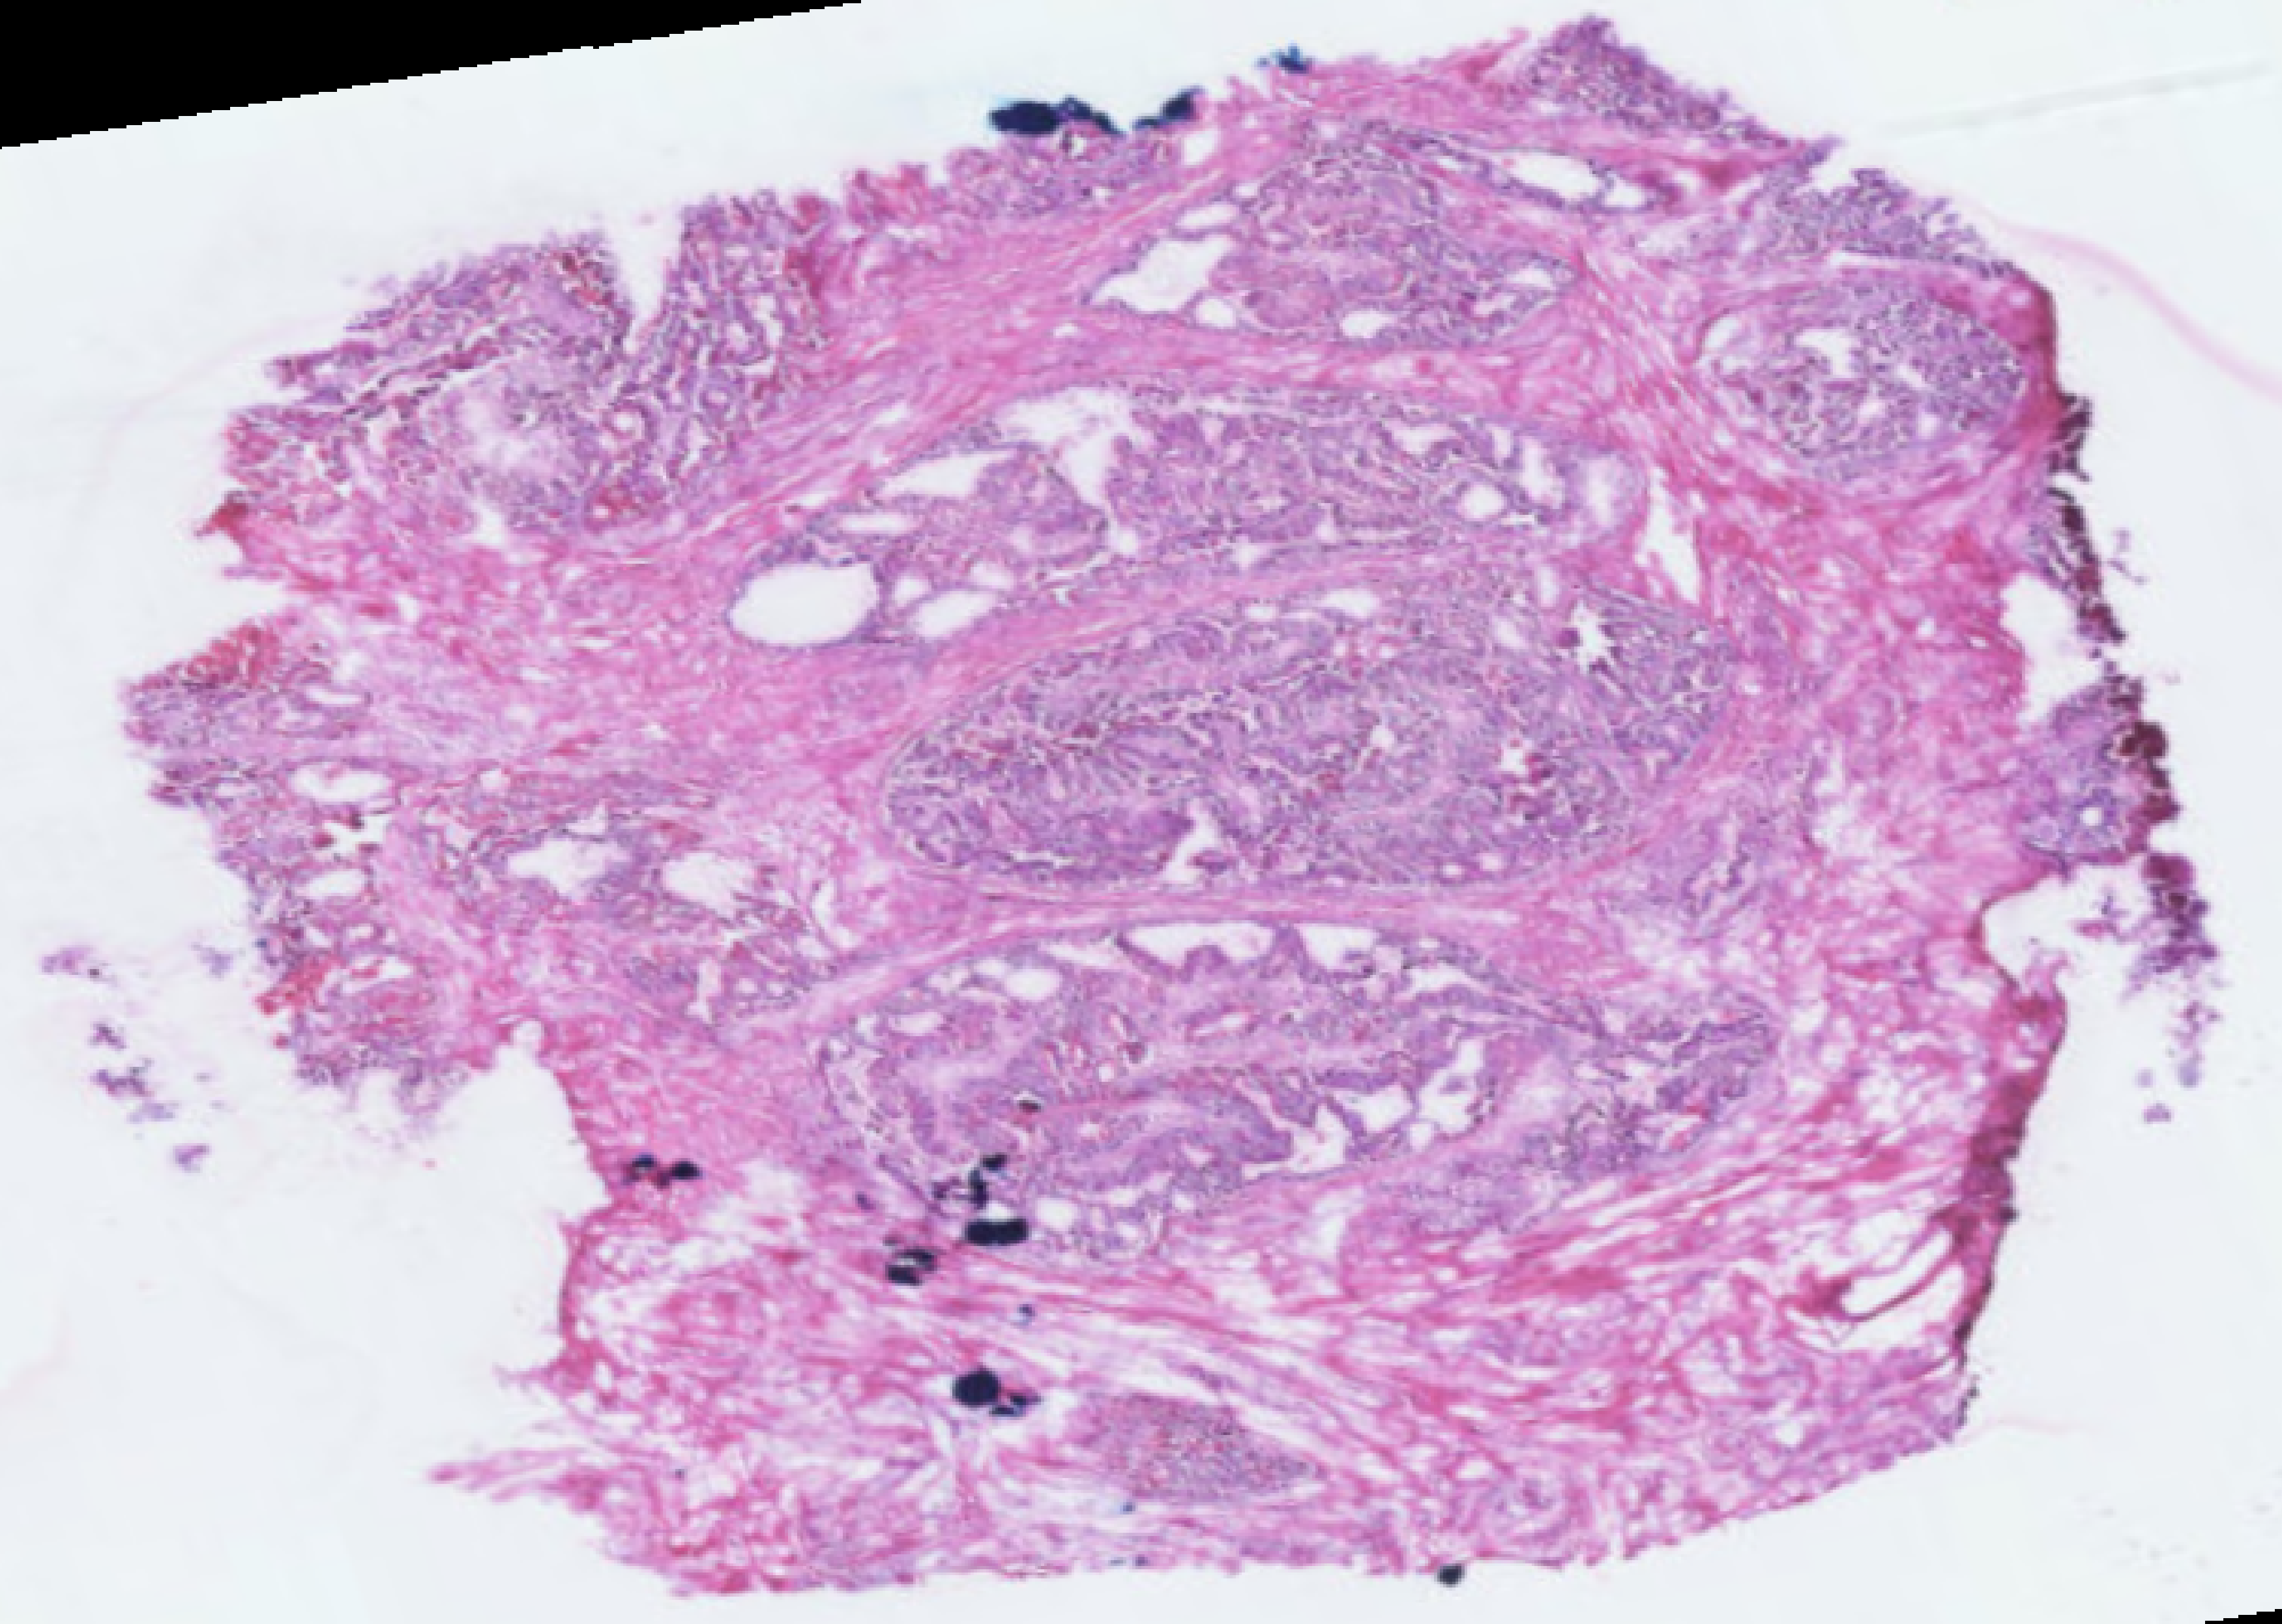
\includegraphics[width=\colWidth\textwidth]{pic/colorectal/s7_op.png}
  %   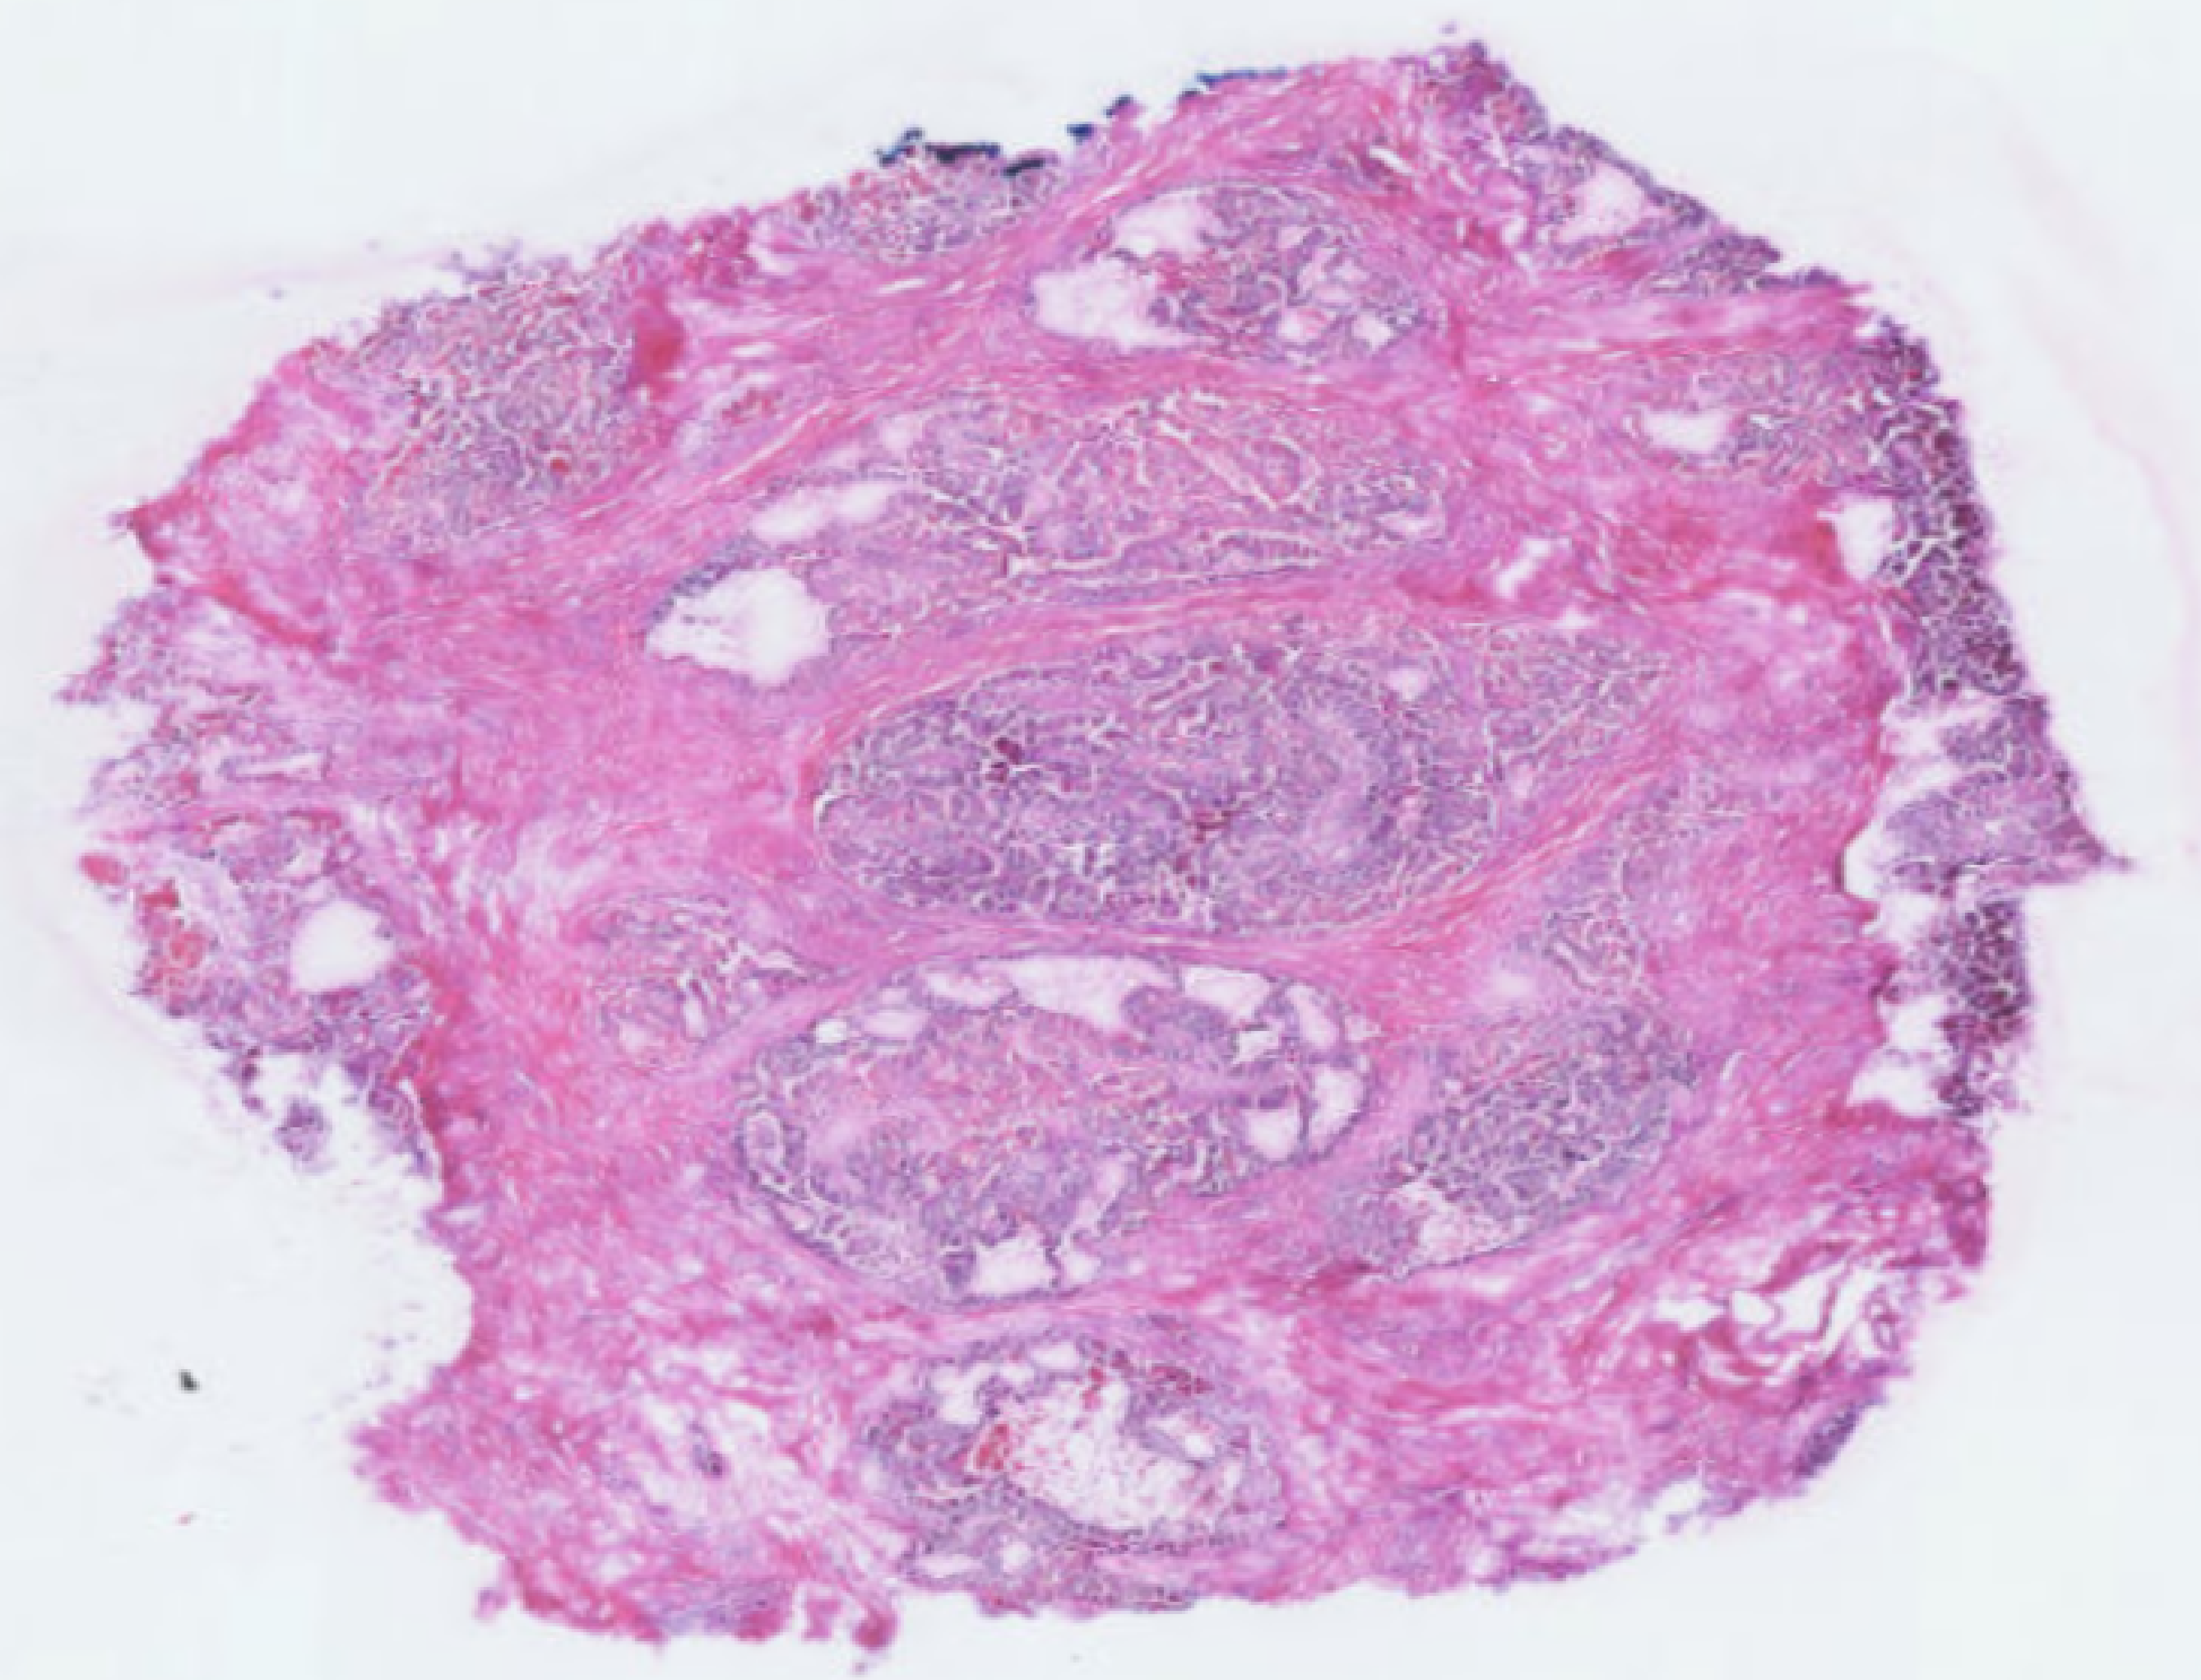
\includegraphics[width=\colWidth\textwidth]{pic/colorectal/s8_op.png}
  %   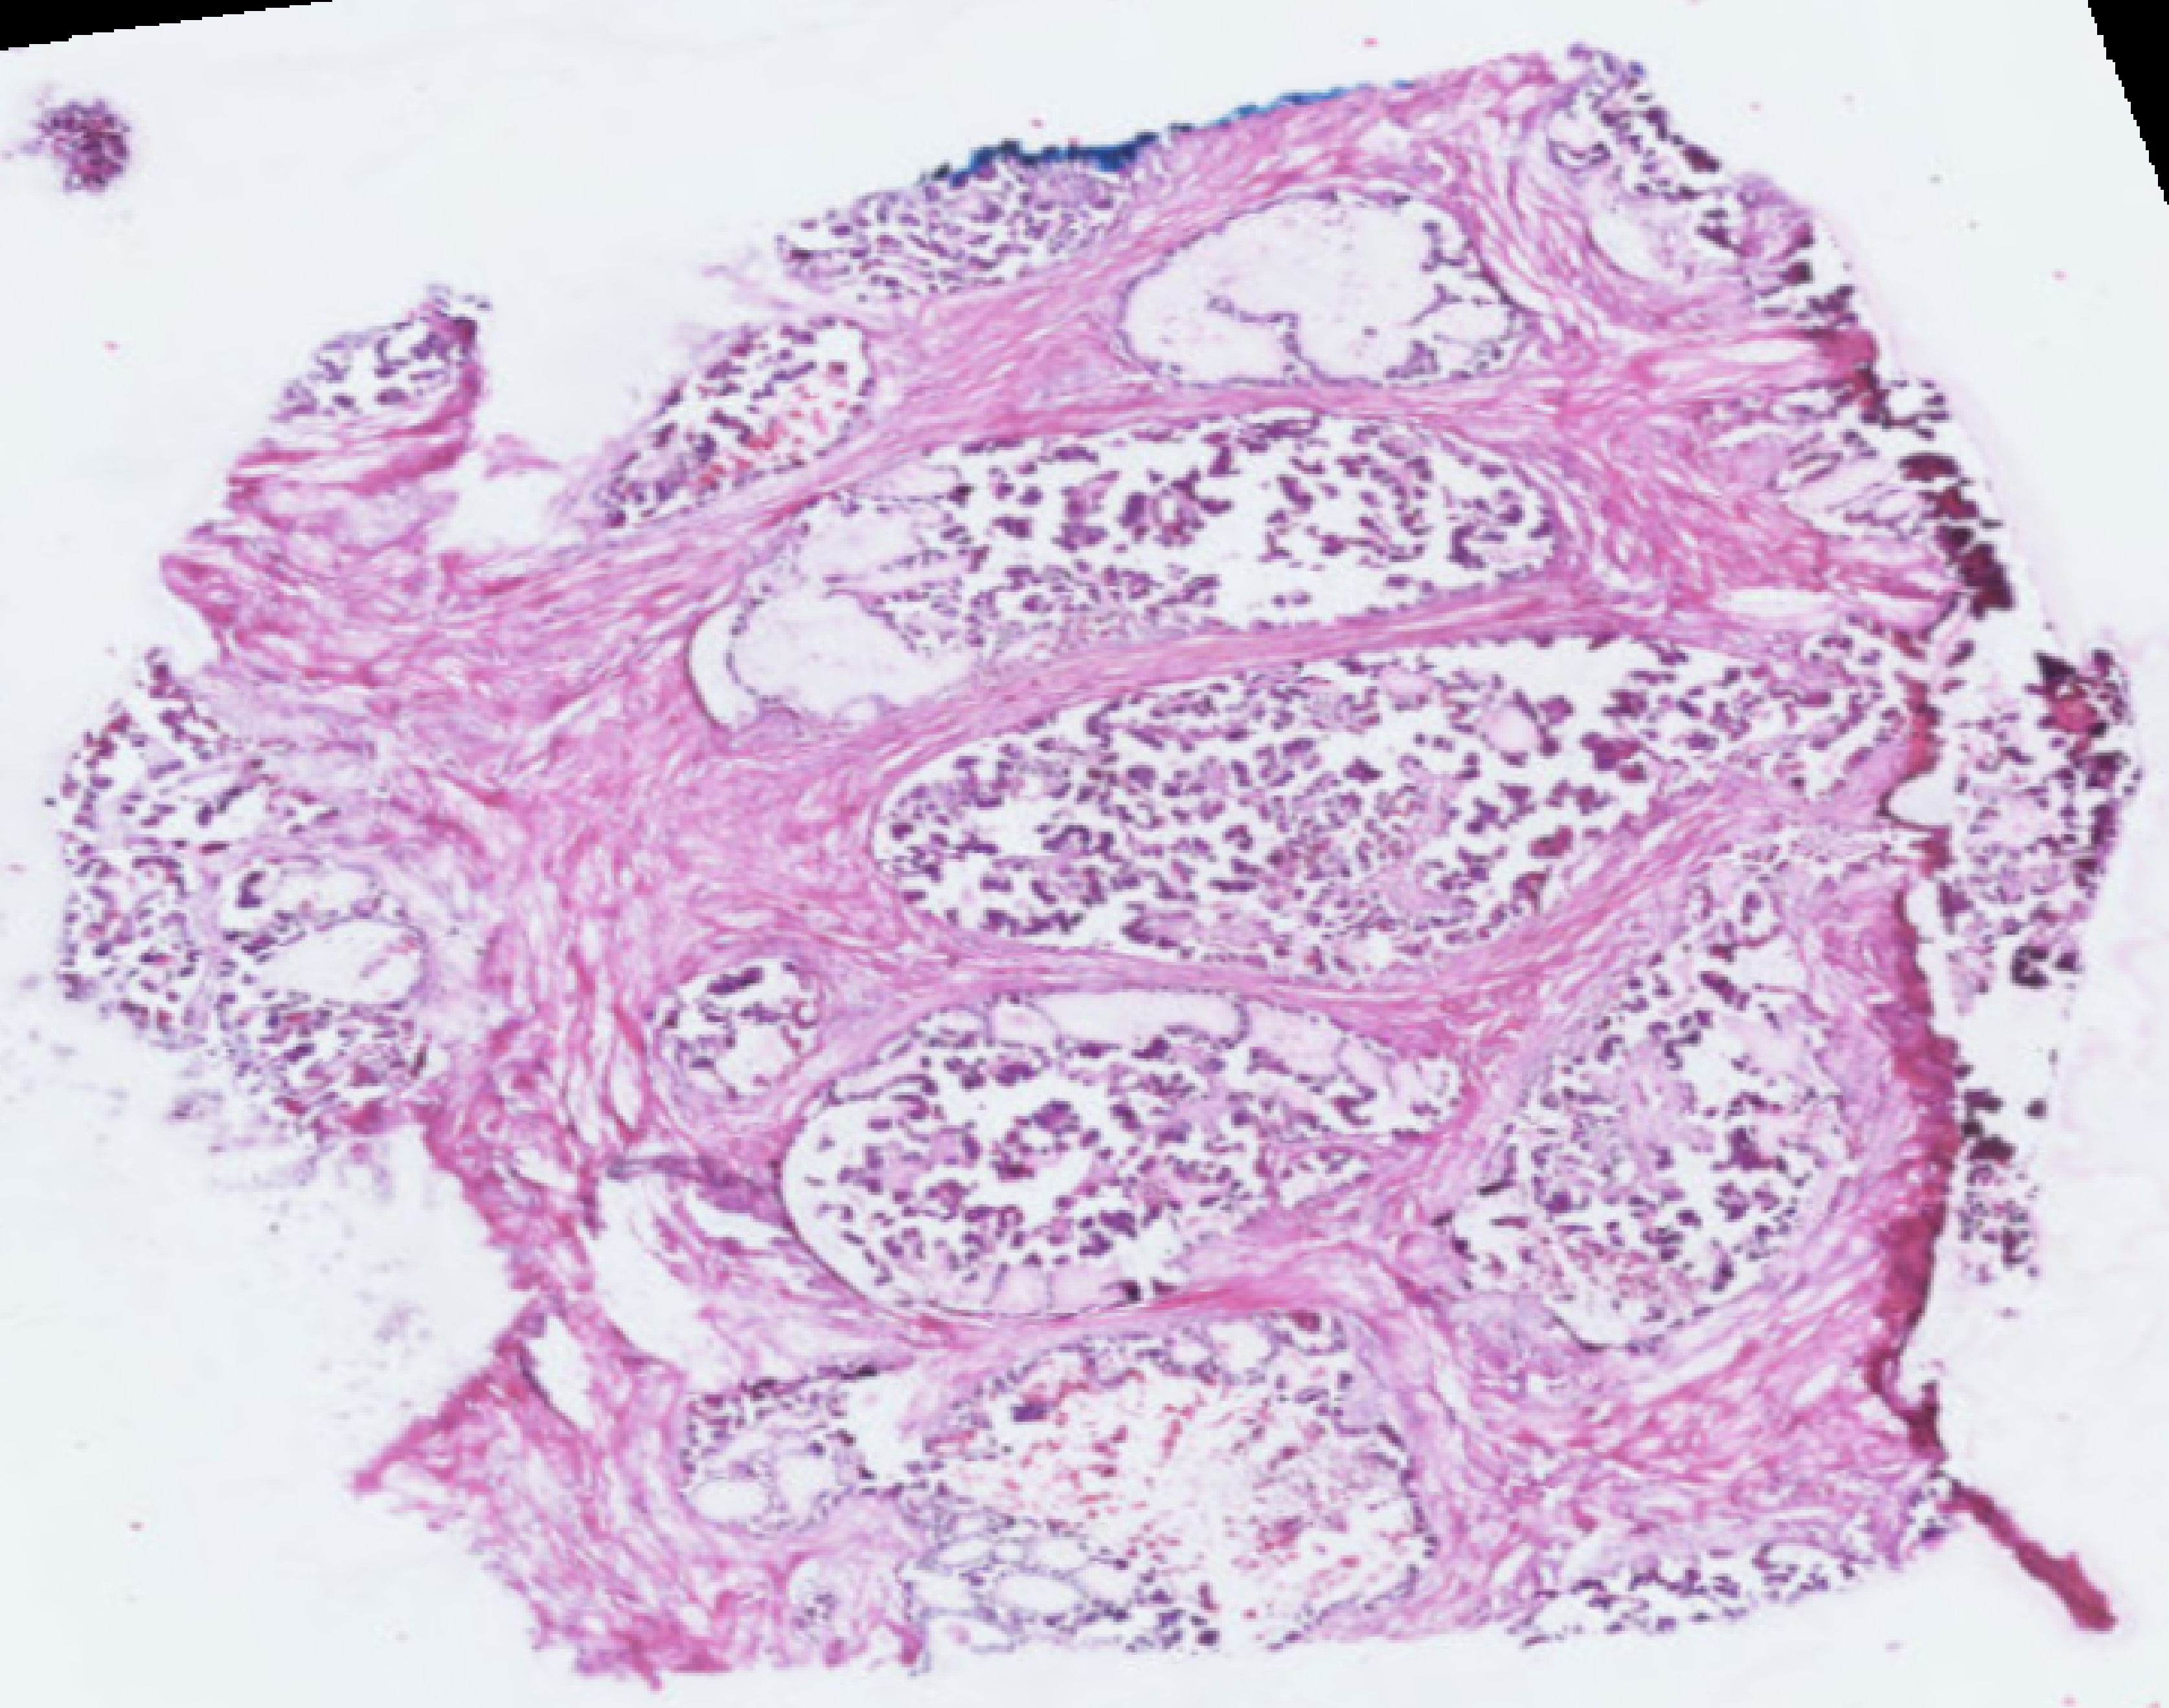
\includegraphics[width=\colWidth\textwidth]{pic/colorectal/s9_op.png}
  %   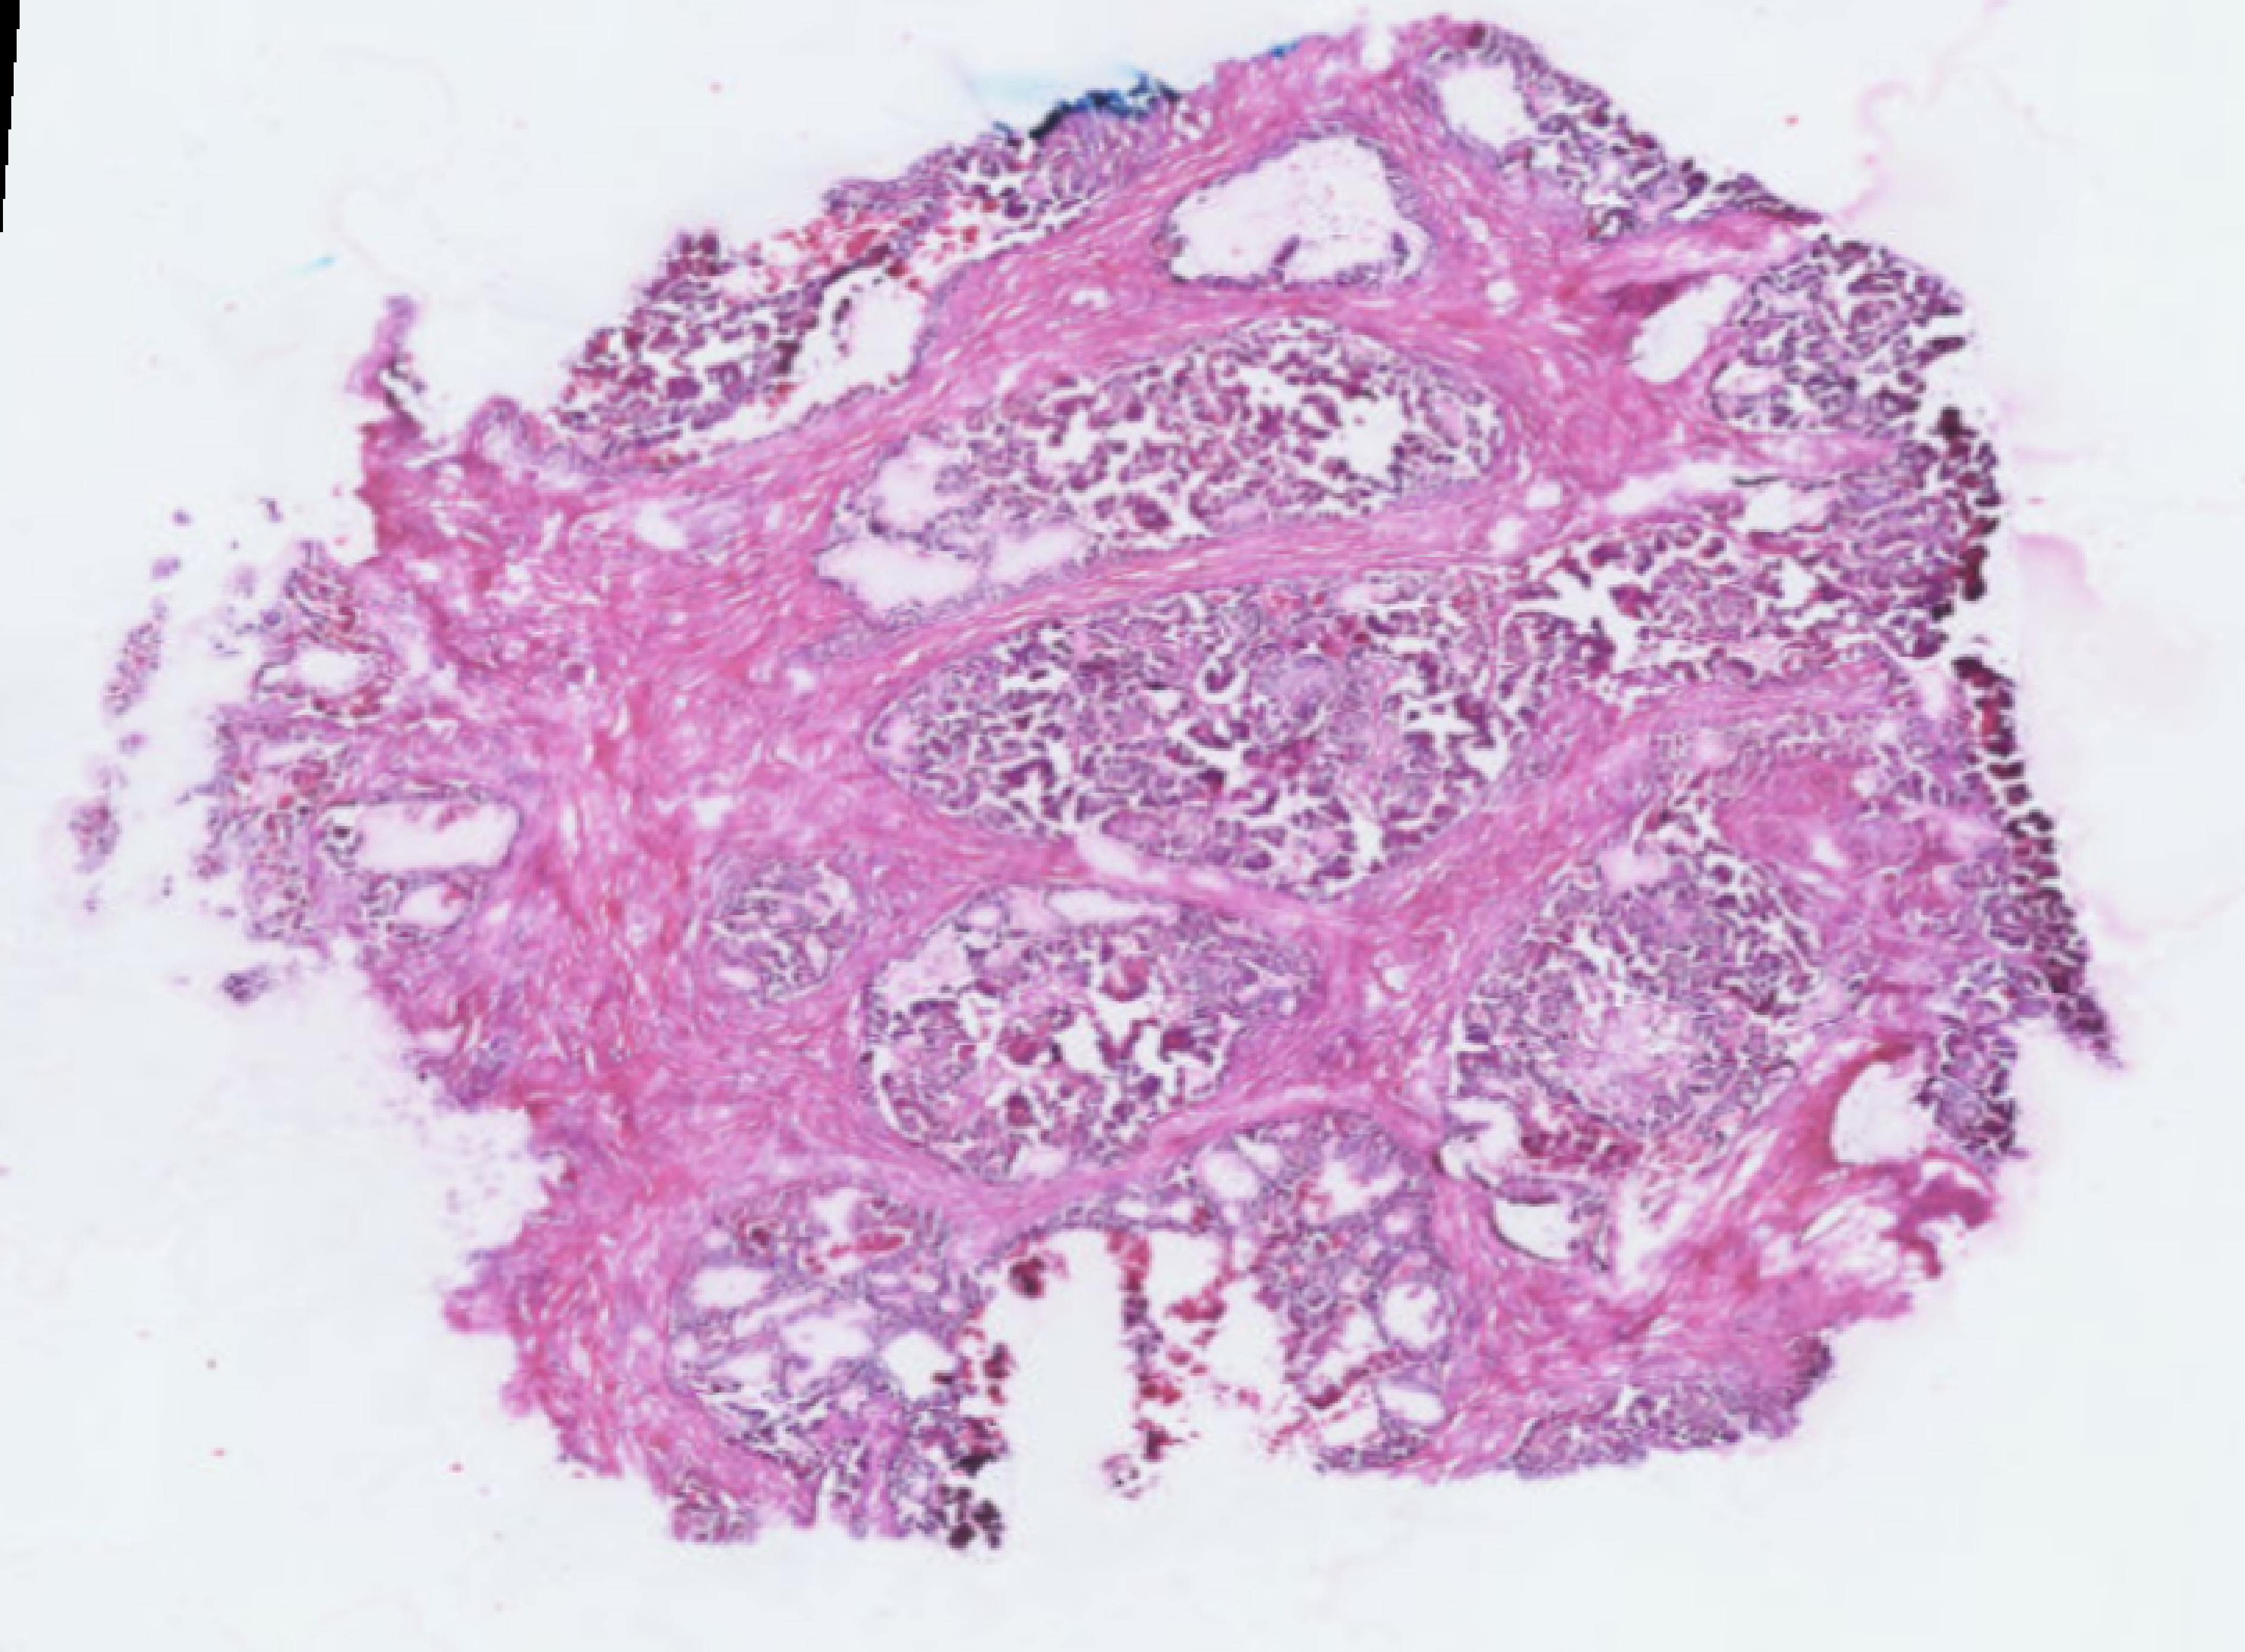
\includegraphics[width=\colWidth\textwidth]{pic/colorectal/s10_op.png}
  %   \\
  %   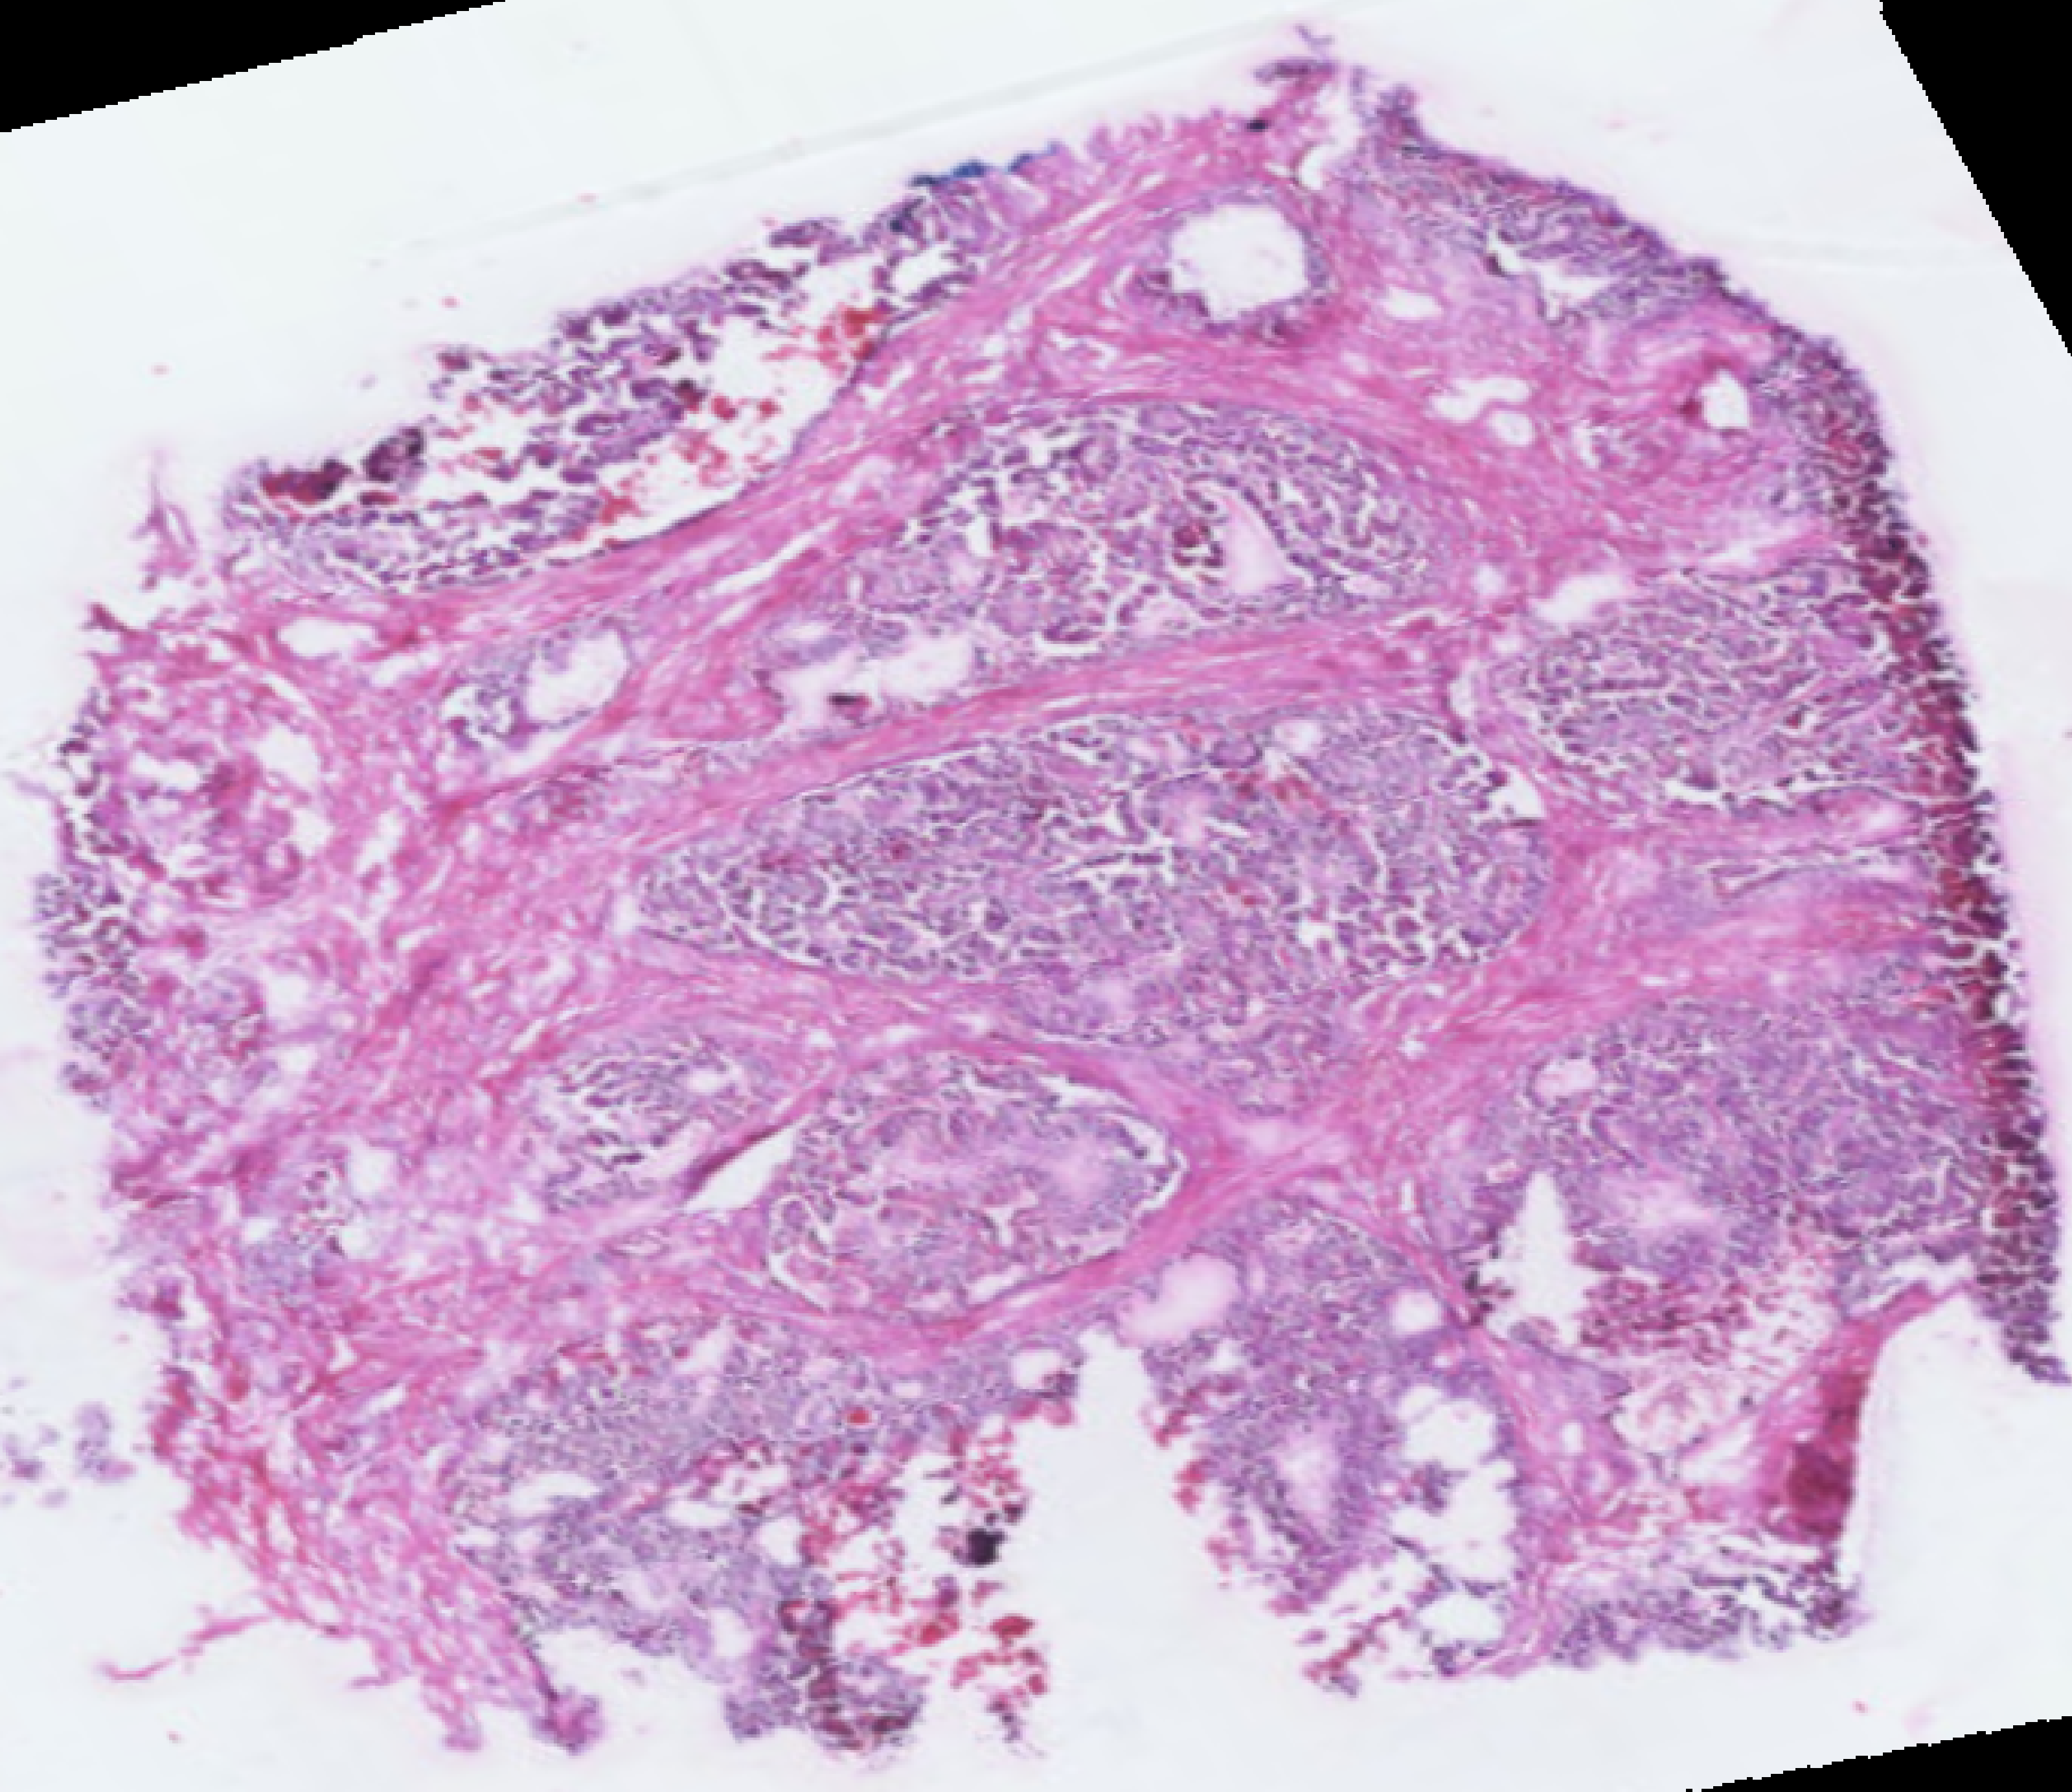
\includegraphics[width=\colWidth\textwidth]{pic/colorectal/s11_op.png}
  %   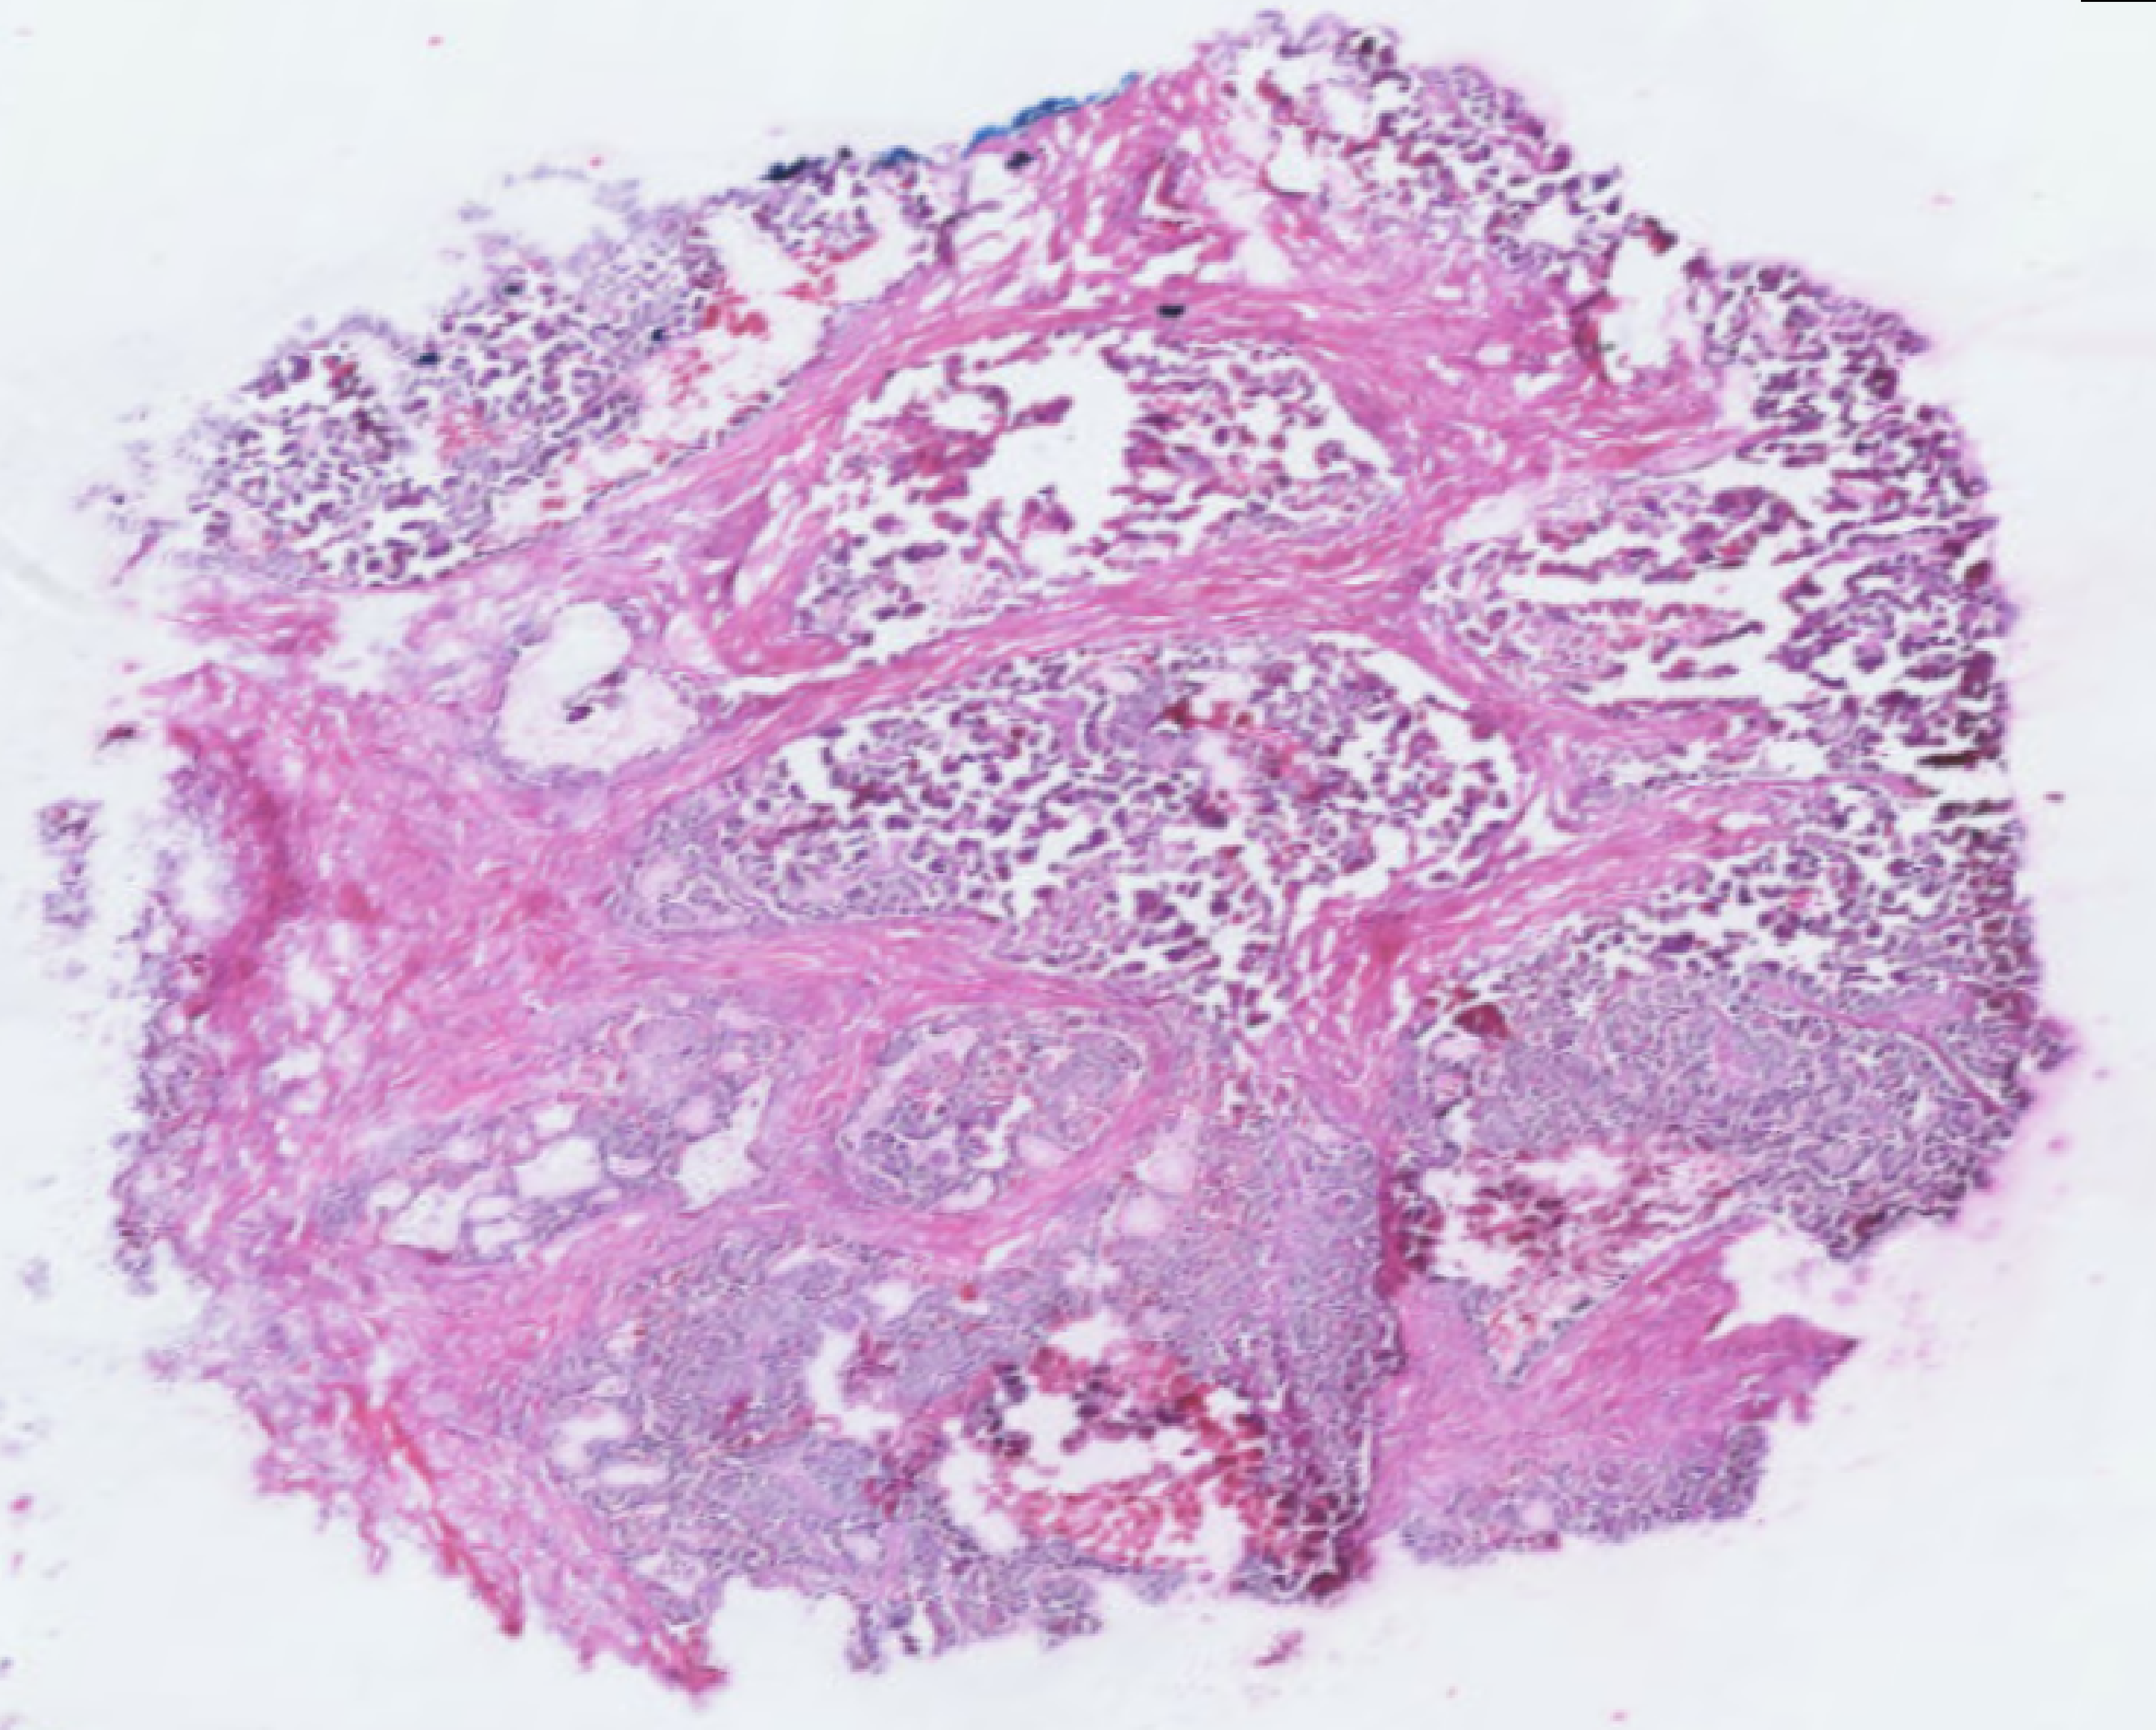
\includegraphics[width=\colWidth\textwidth]{pic/colorectal/s12_op.png}
  %   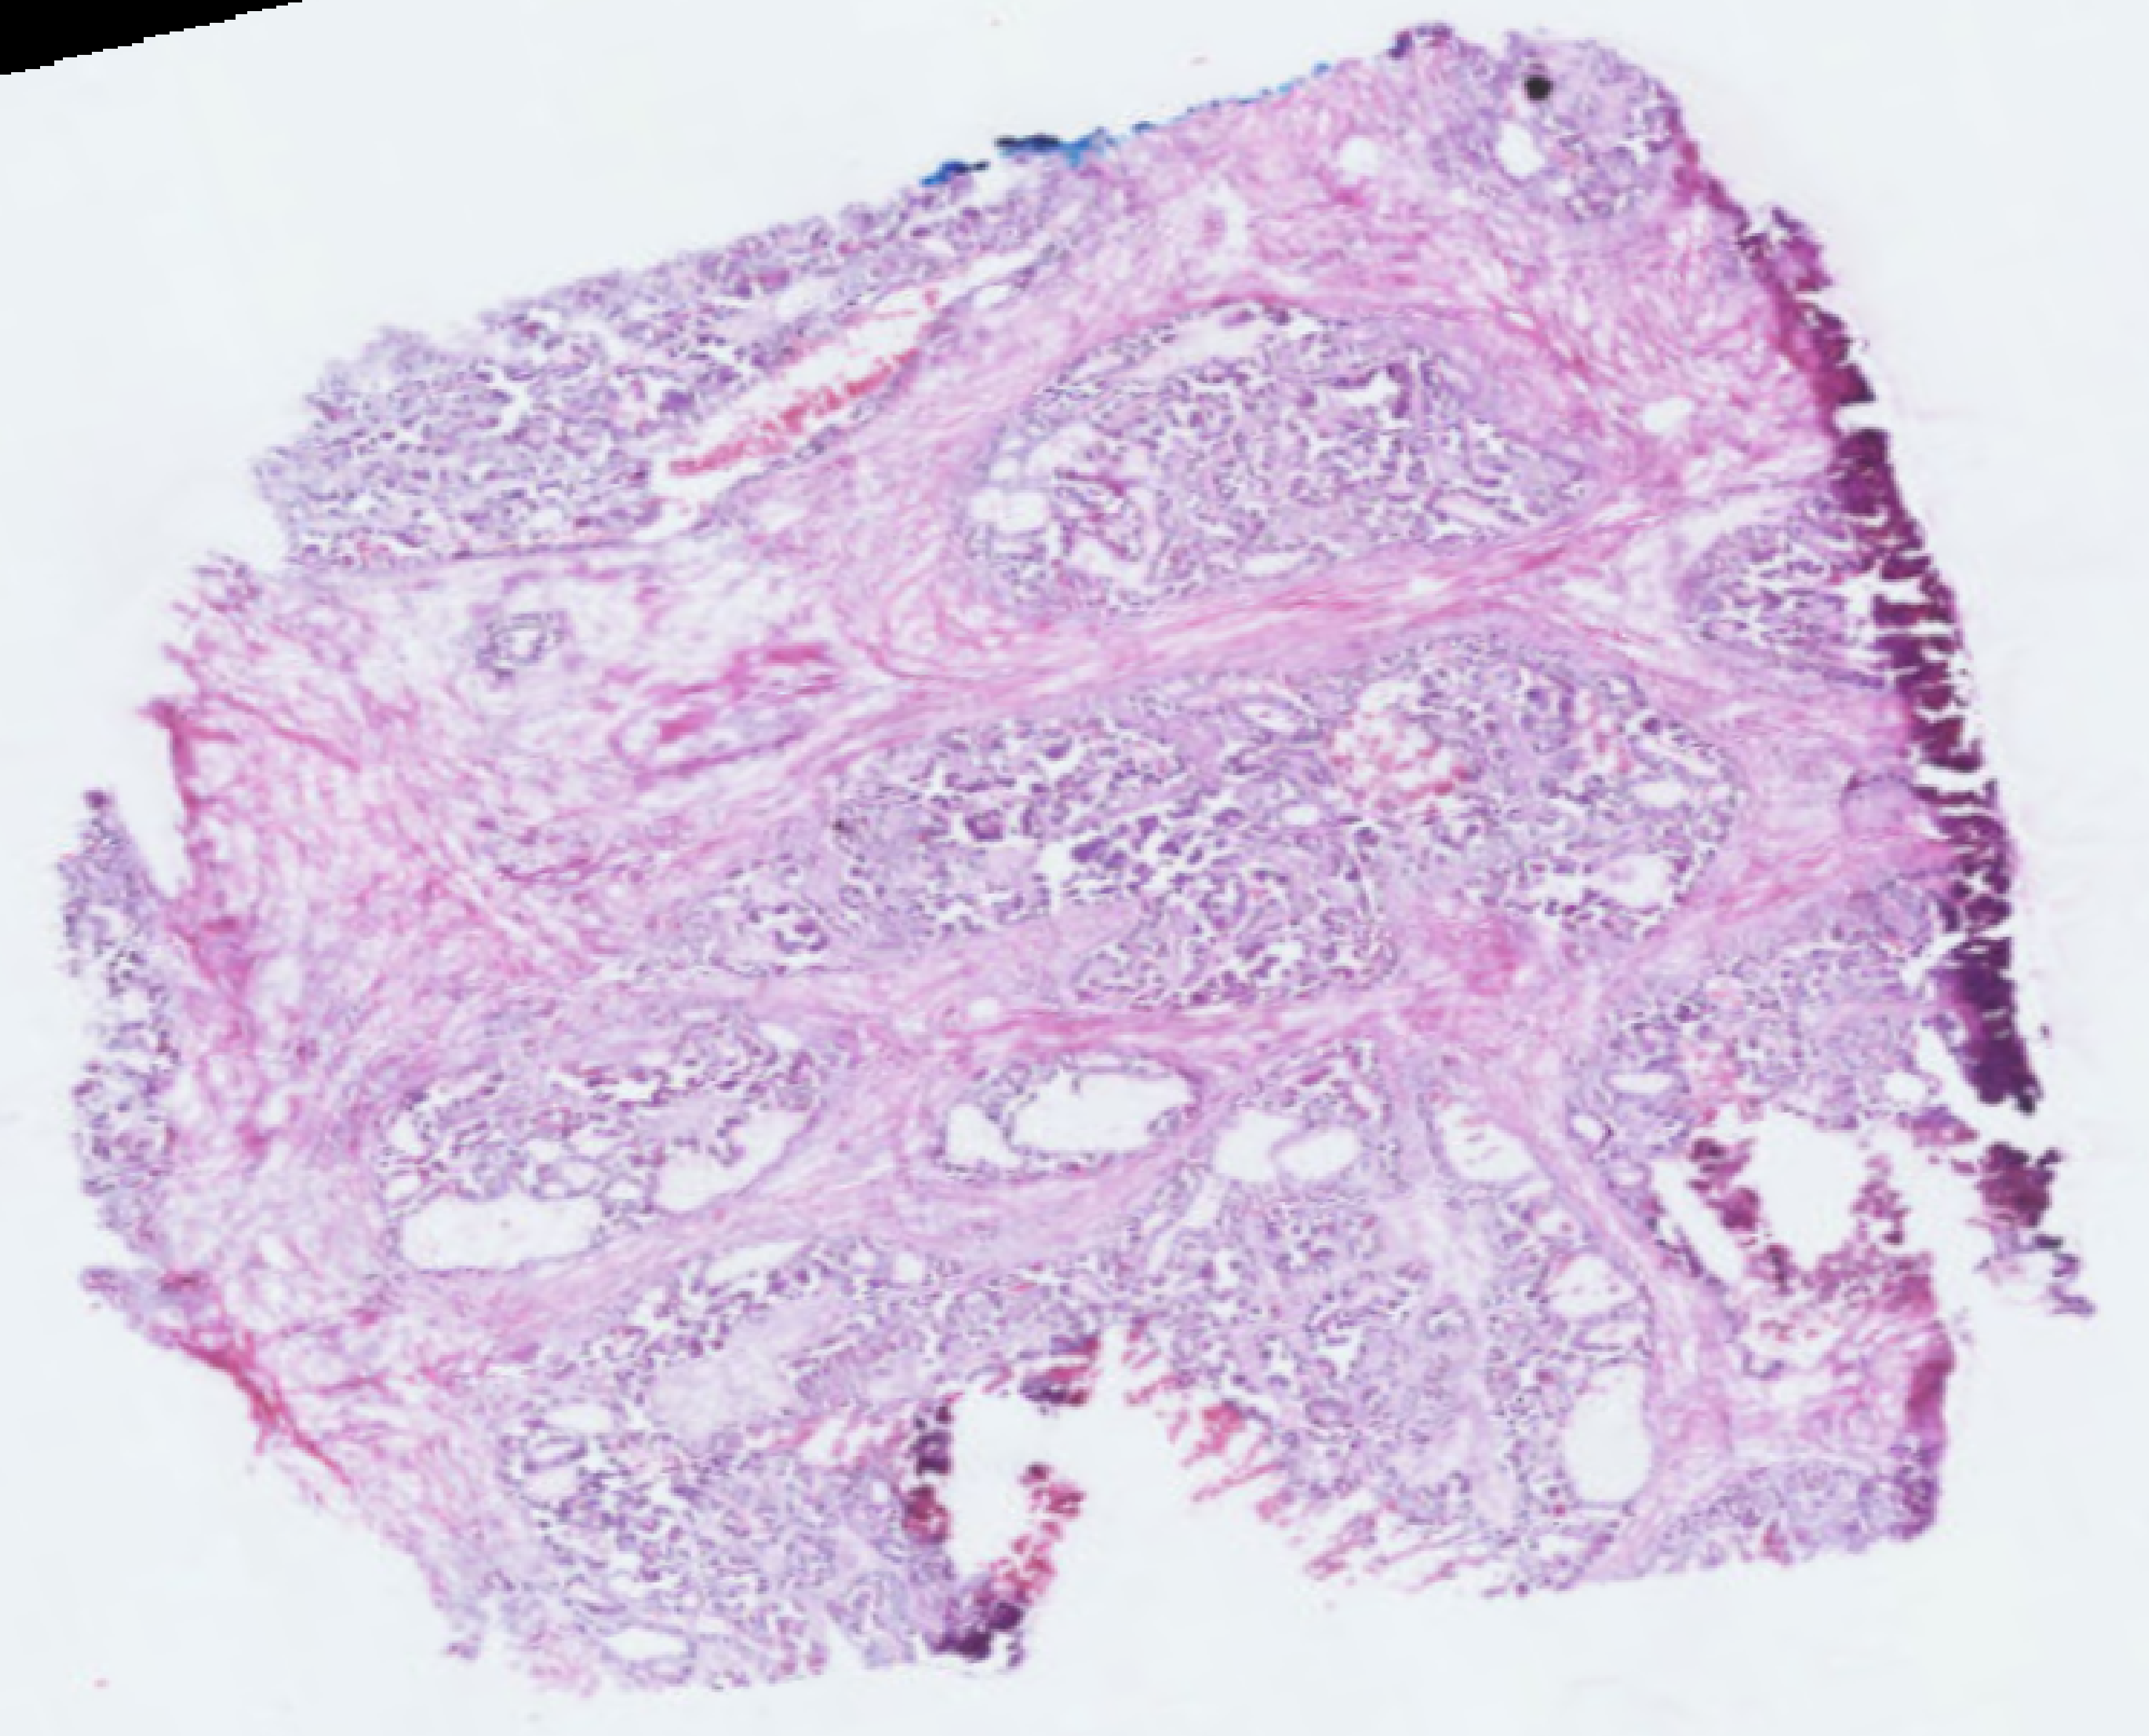
\includegraphics[width=\colWidth\textwidth]{pic/colorectal/s13_op.png}
  %   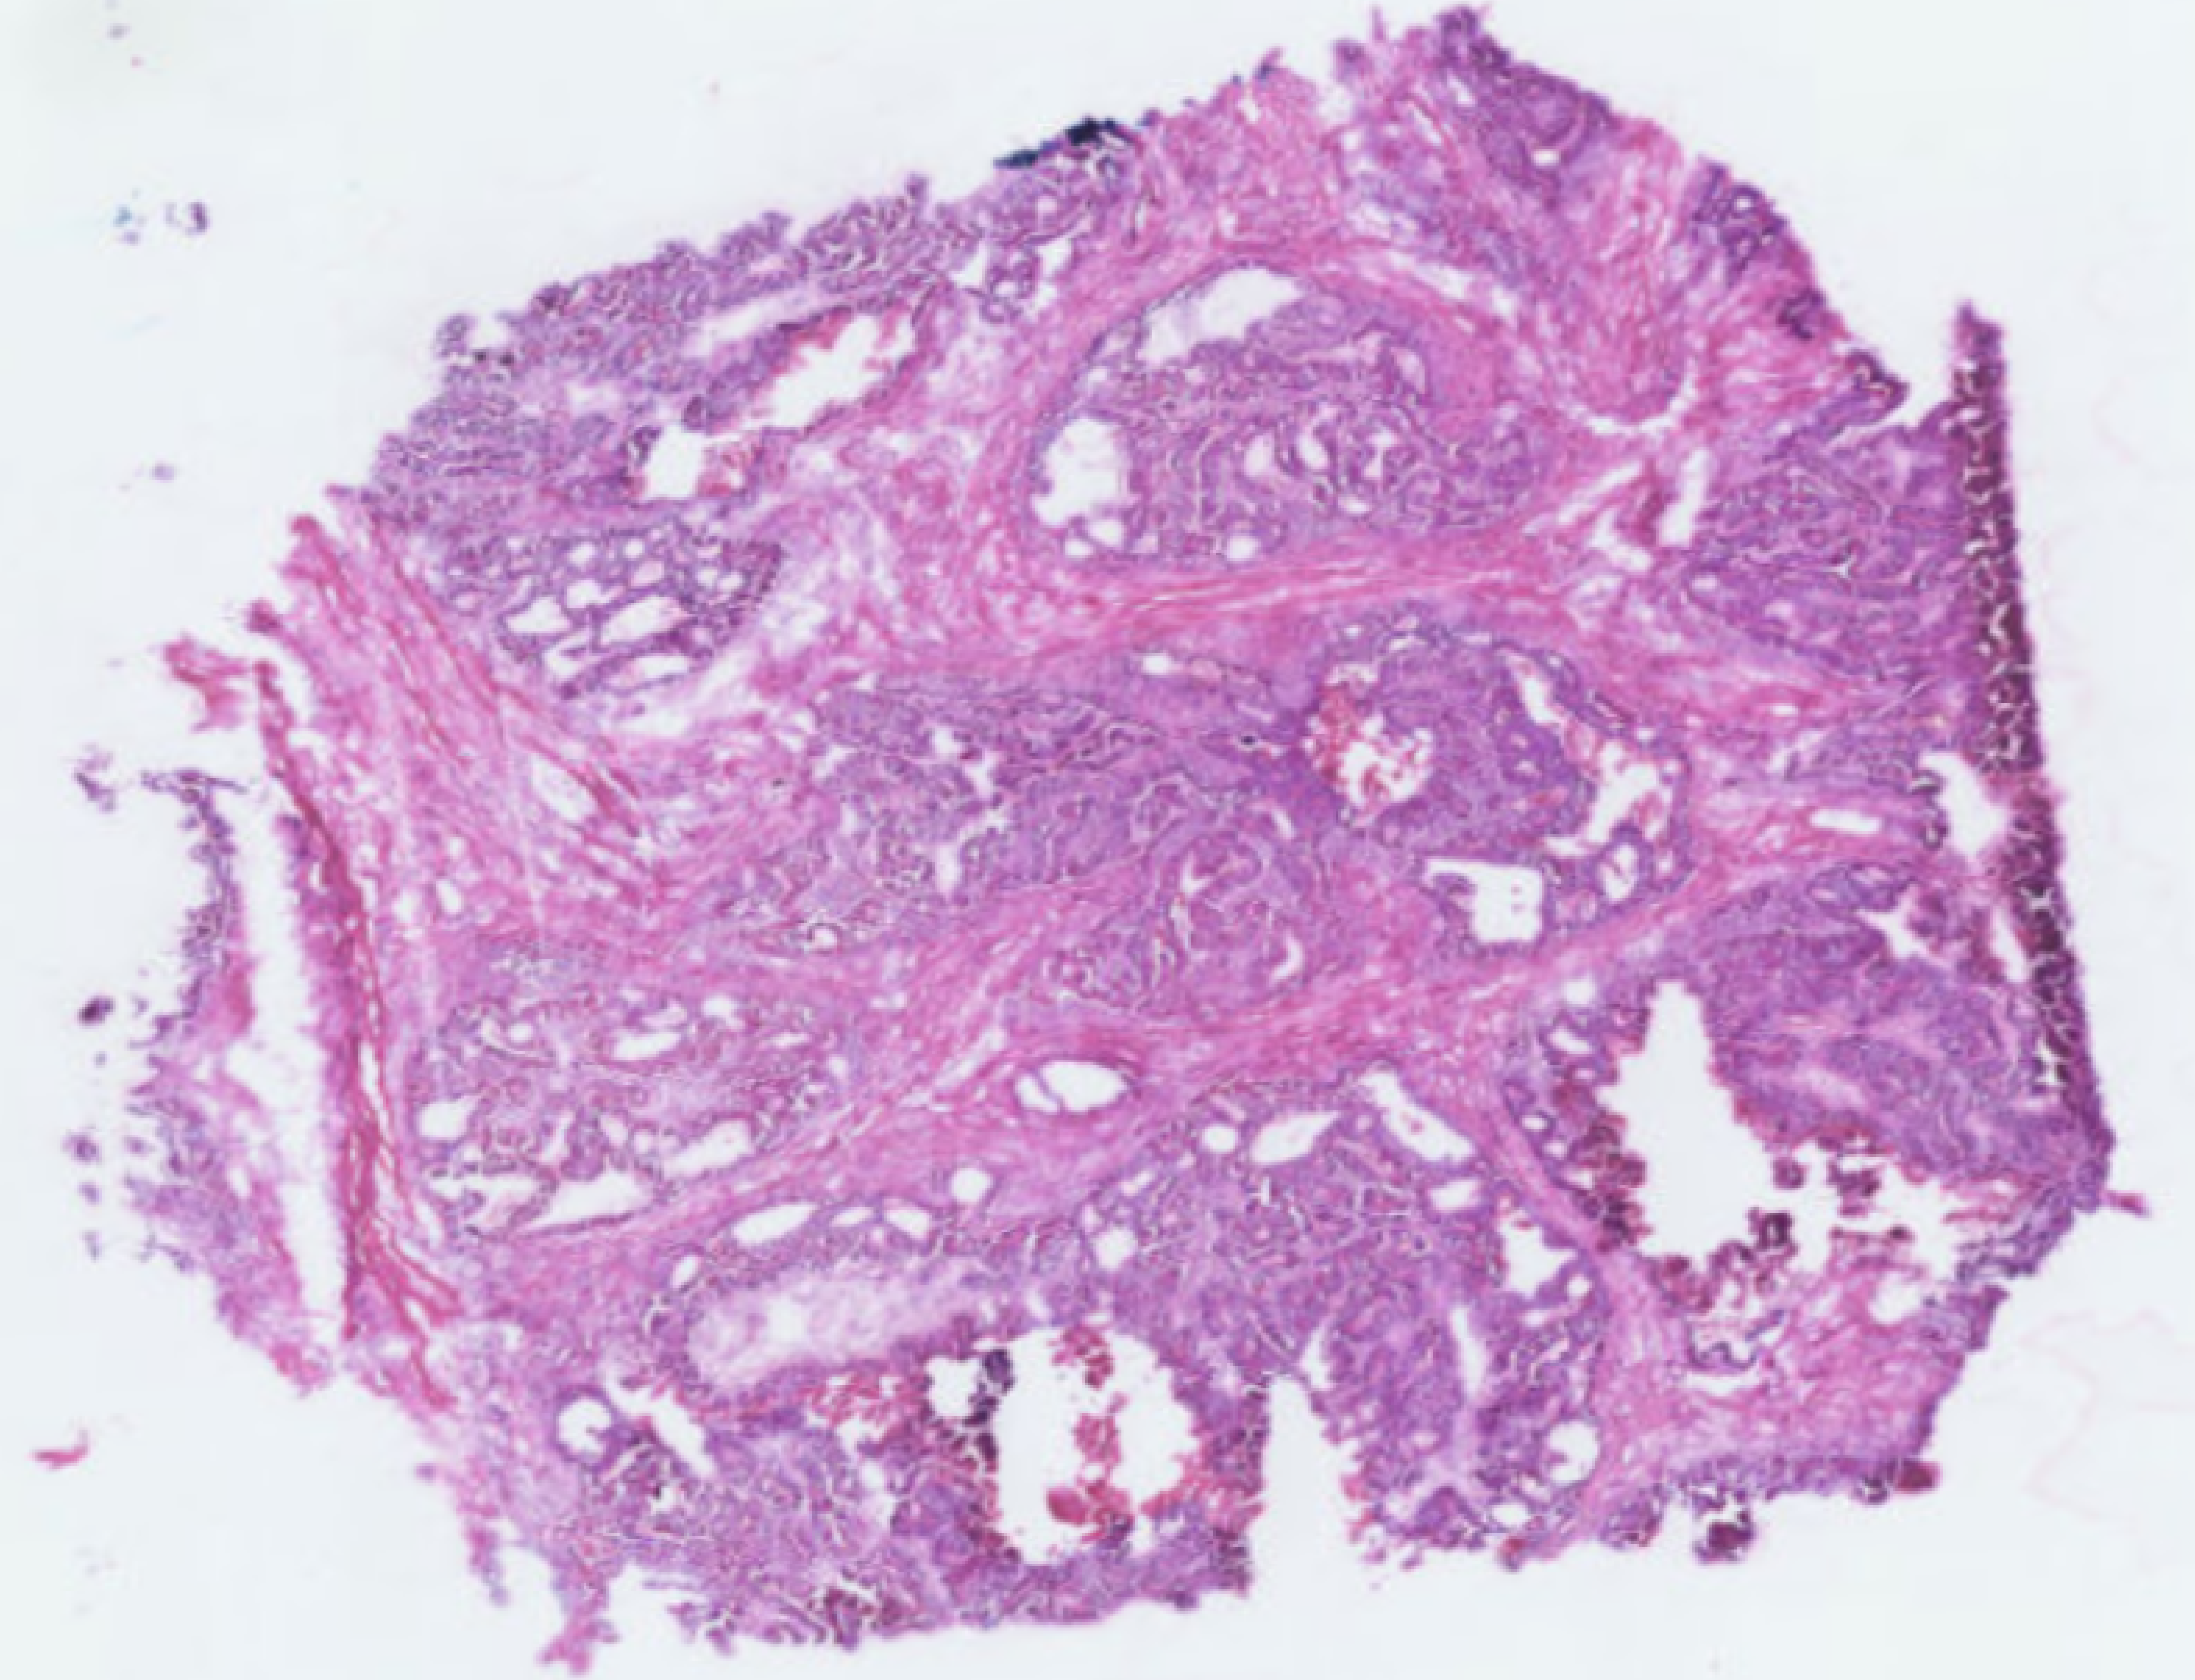
\includegraphics[width=\colWidth\textwidth]{pic/colorectal/s14_op.png}
  %   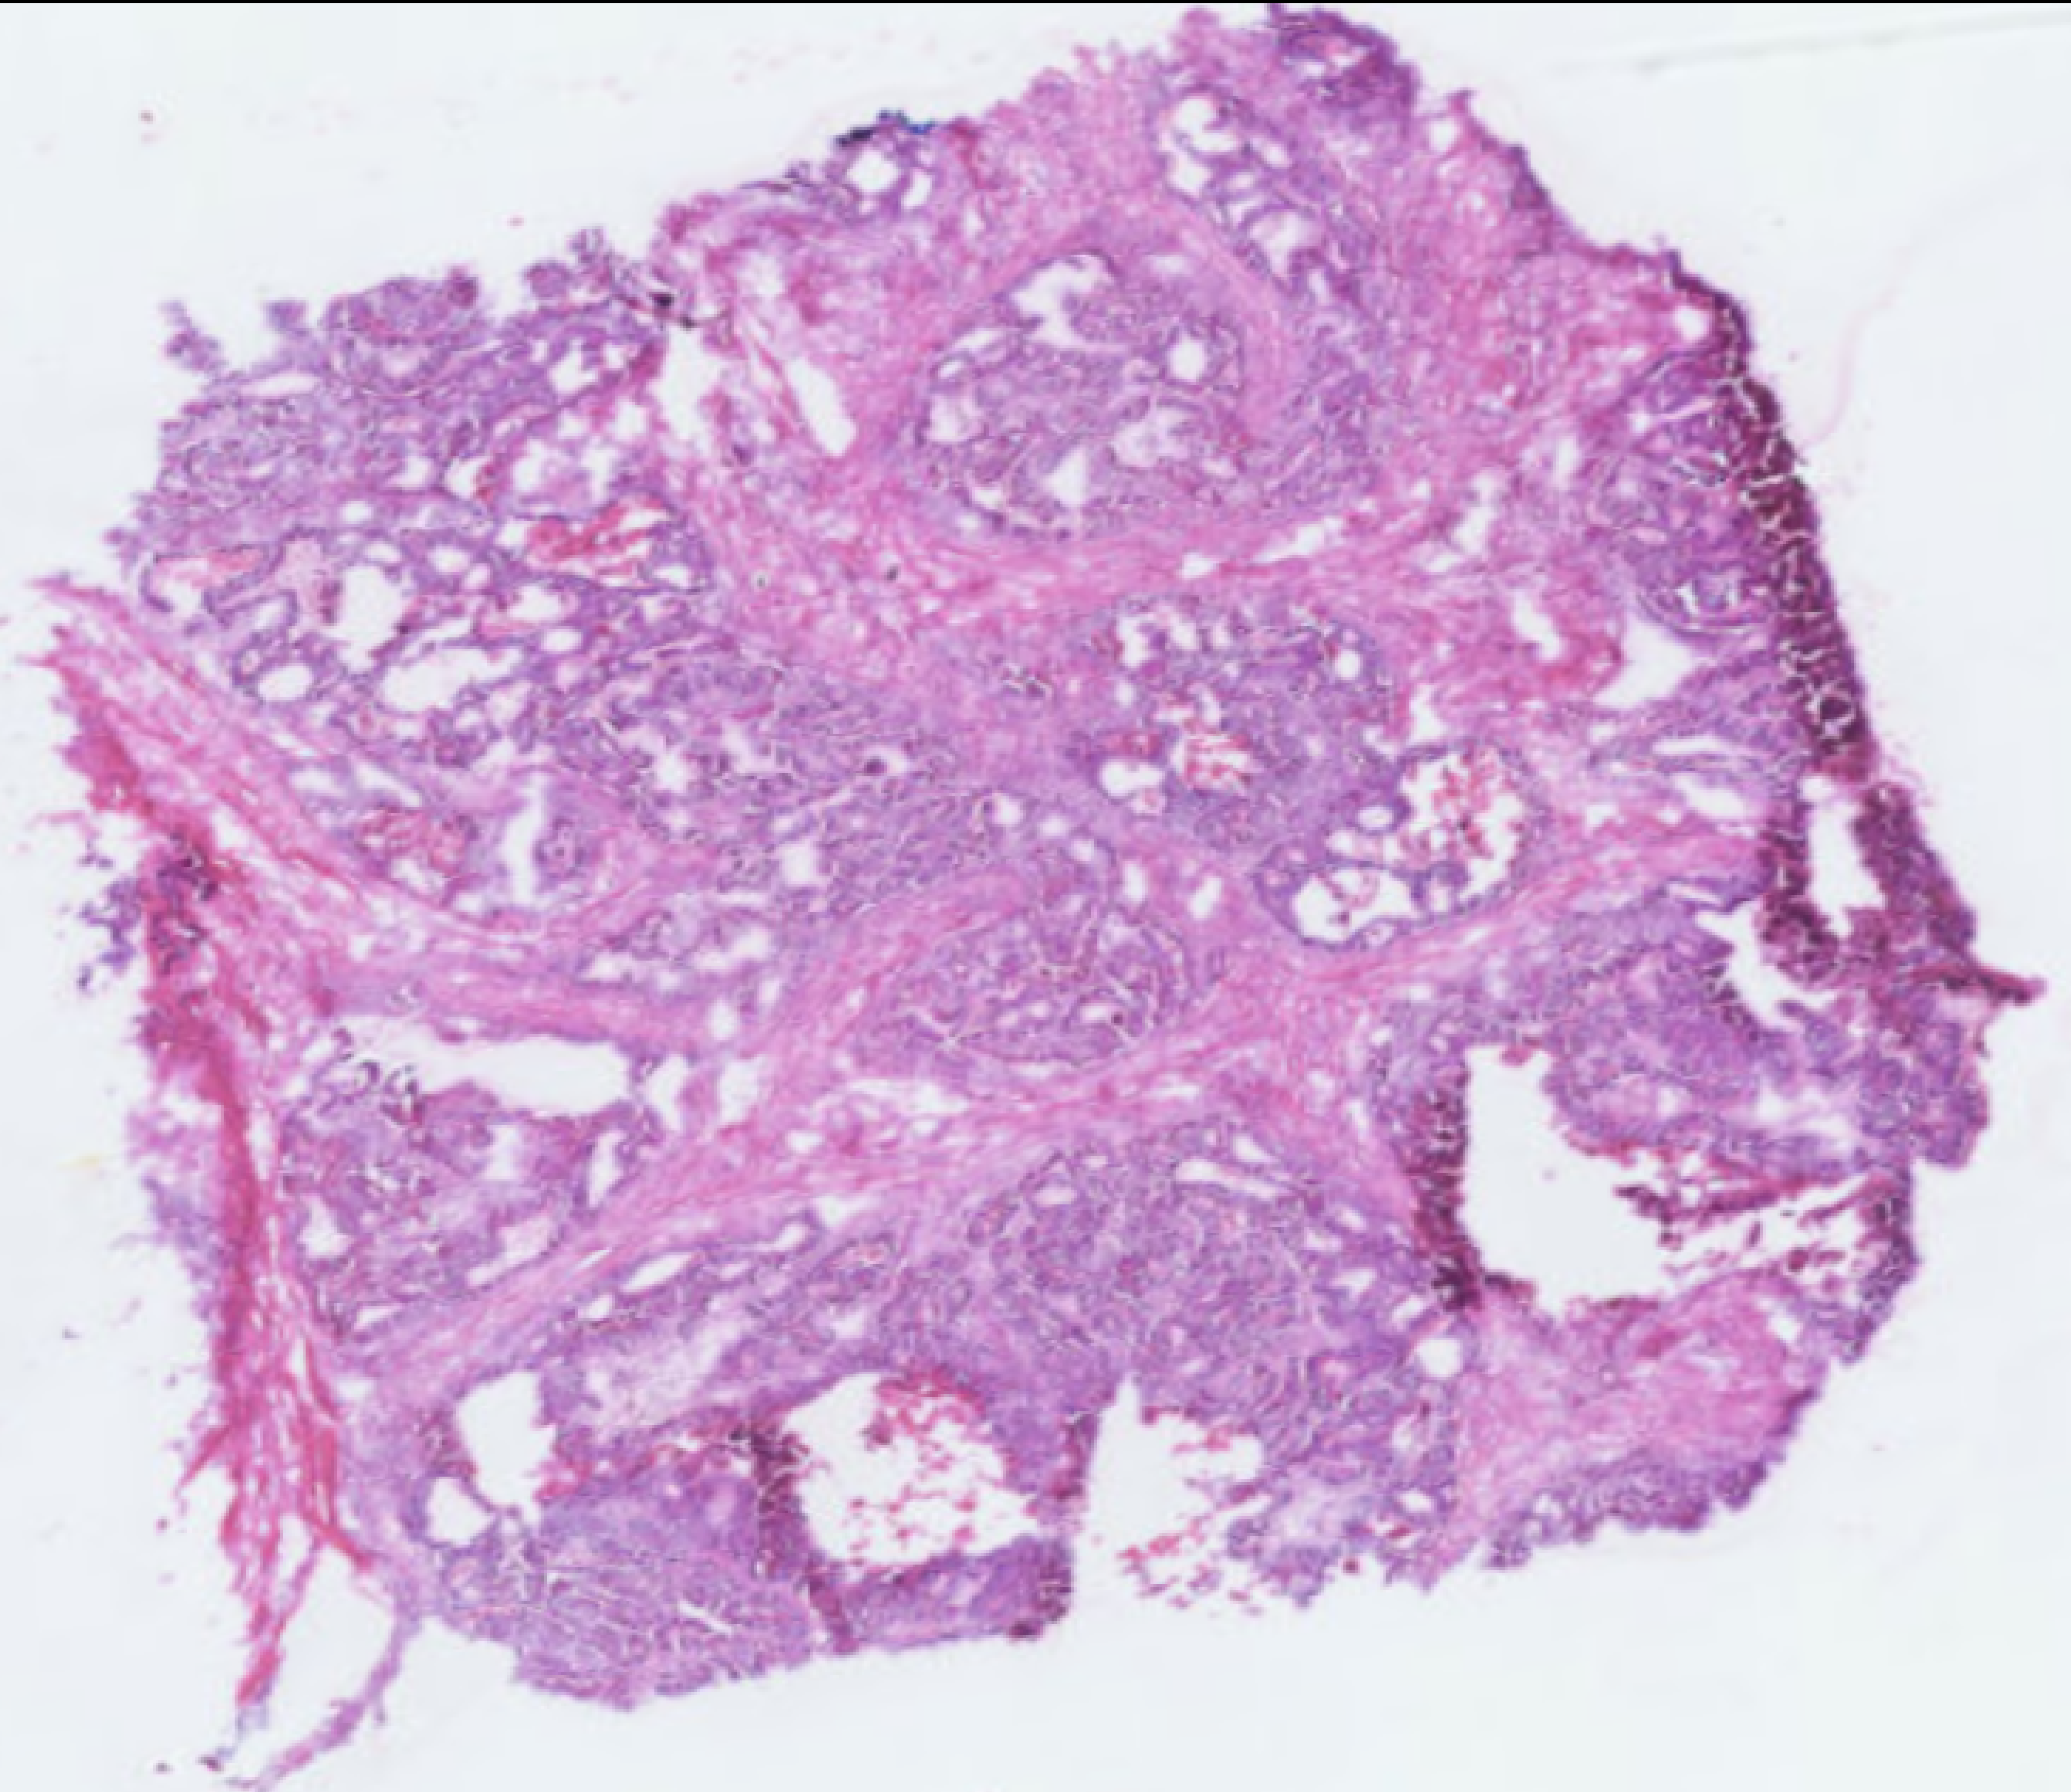
\includegraphics[width=\colWidth\textwidth]{pic/colorectal/s15_op.png}
  %   \\
  %   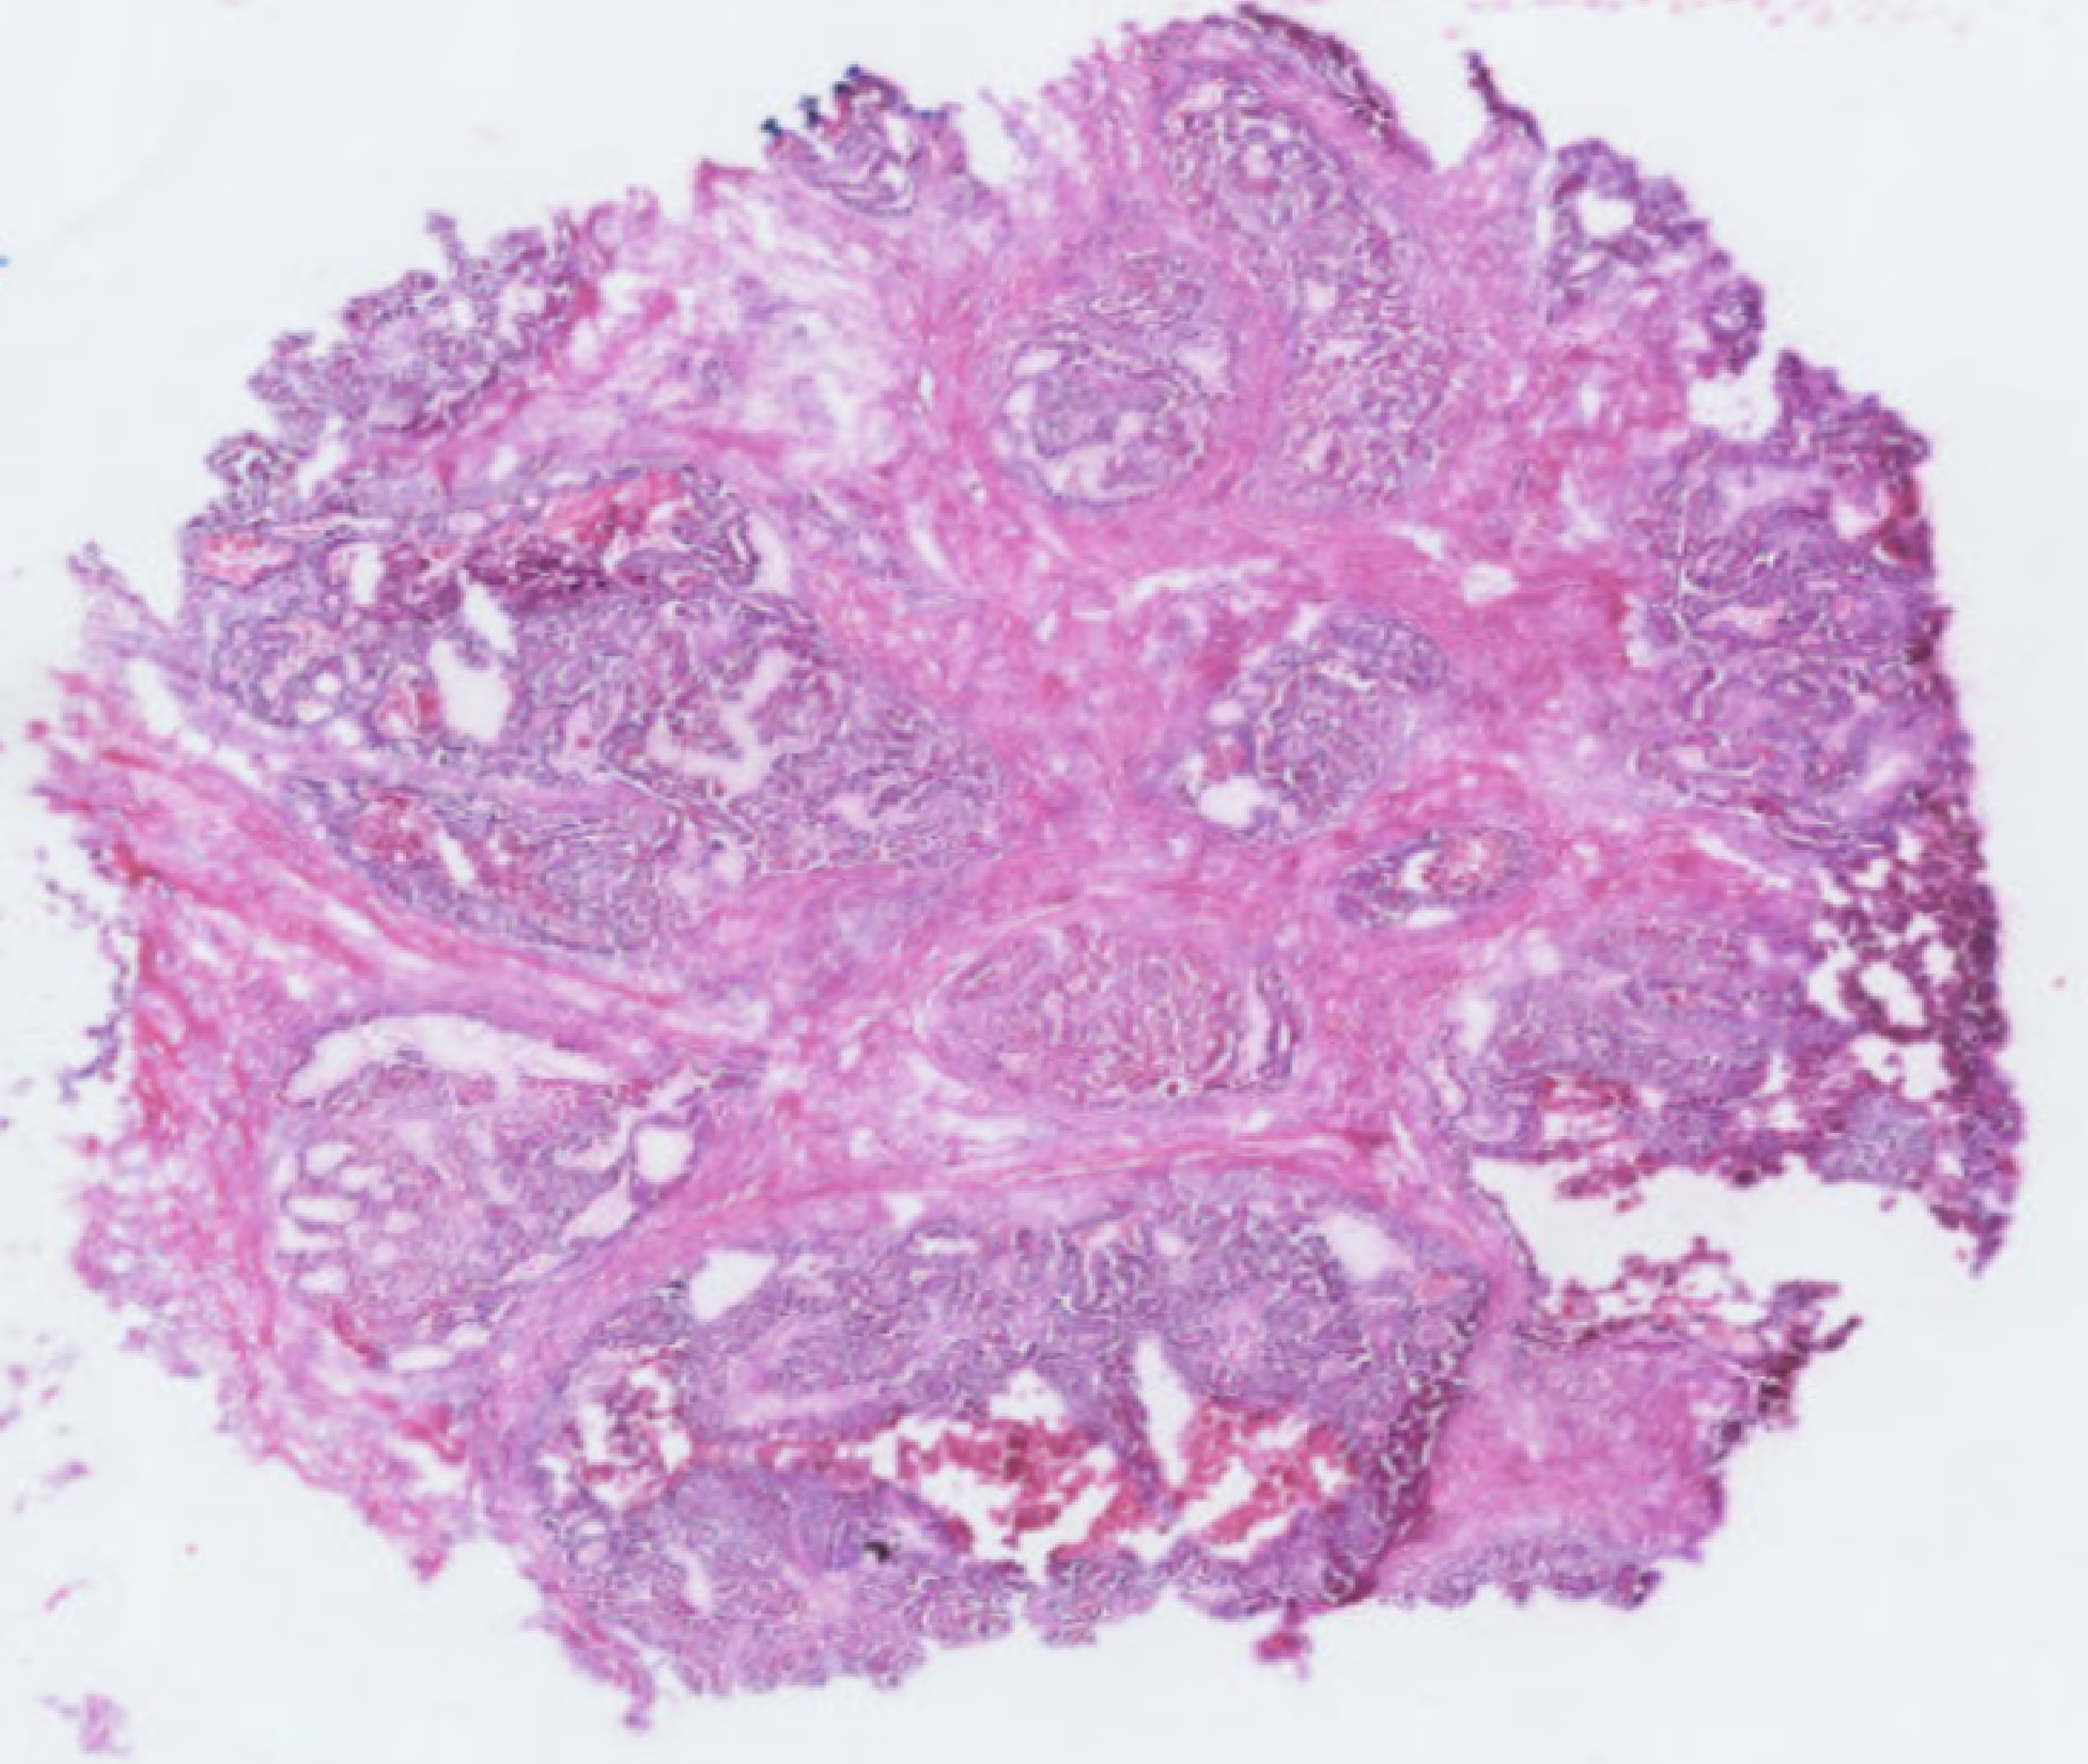
\includegraphics[width=\colWidth\textwidth]{pic/colorectal/s16_op.png}
  %   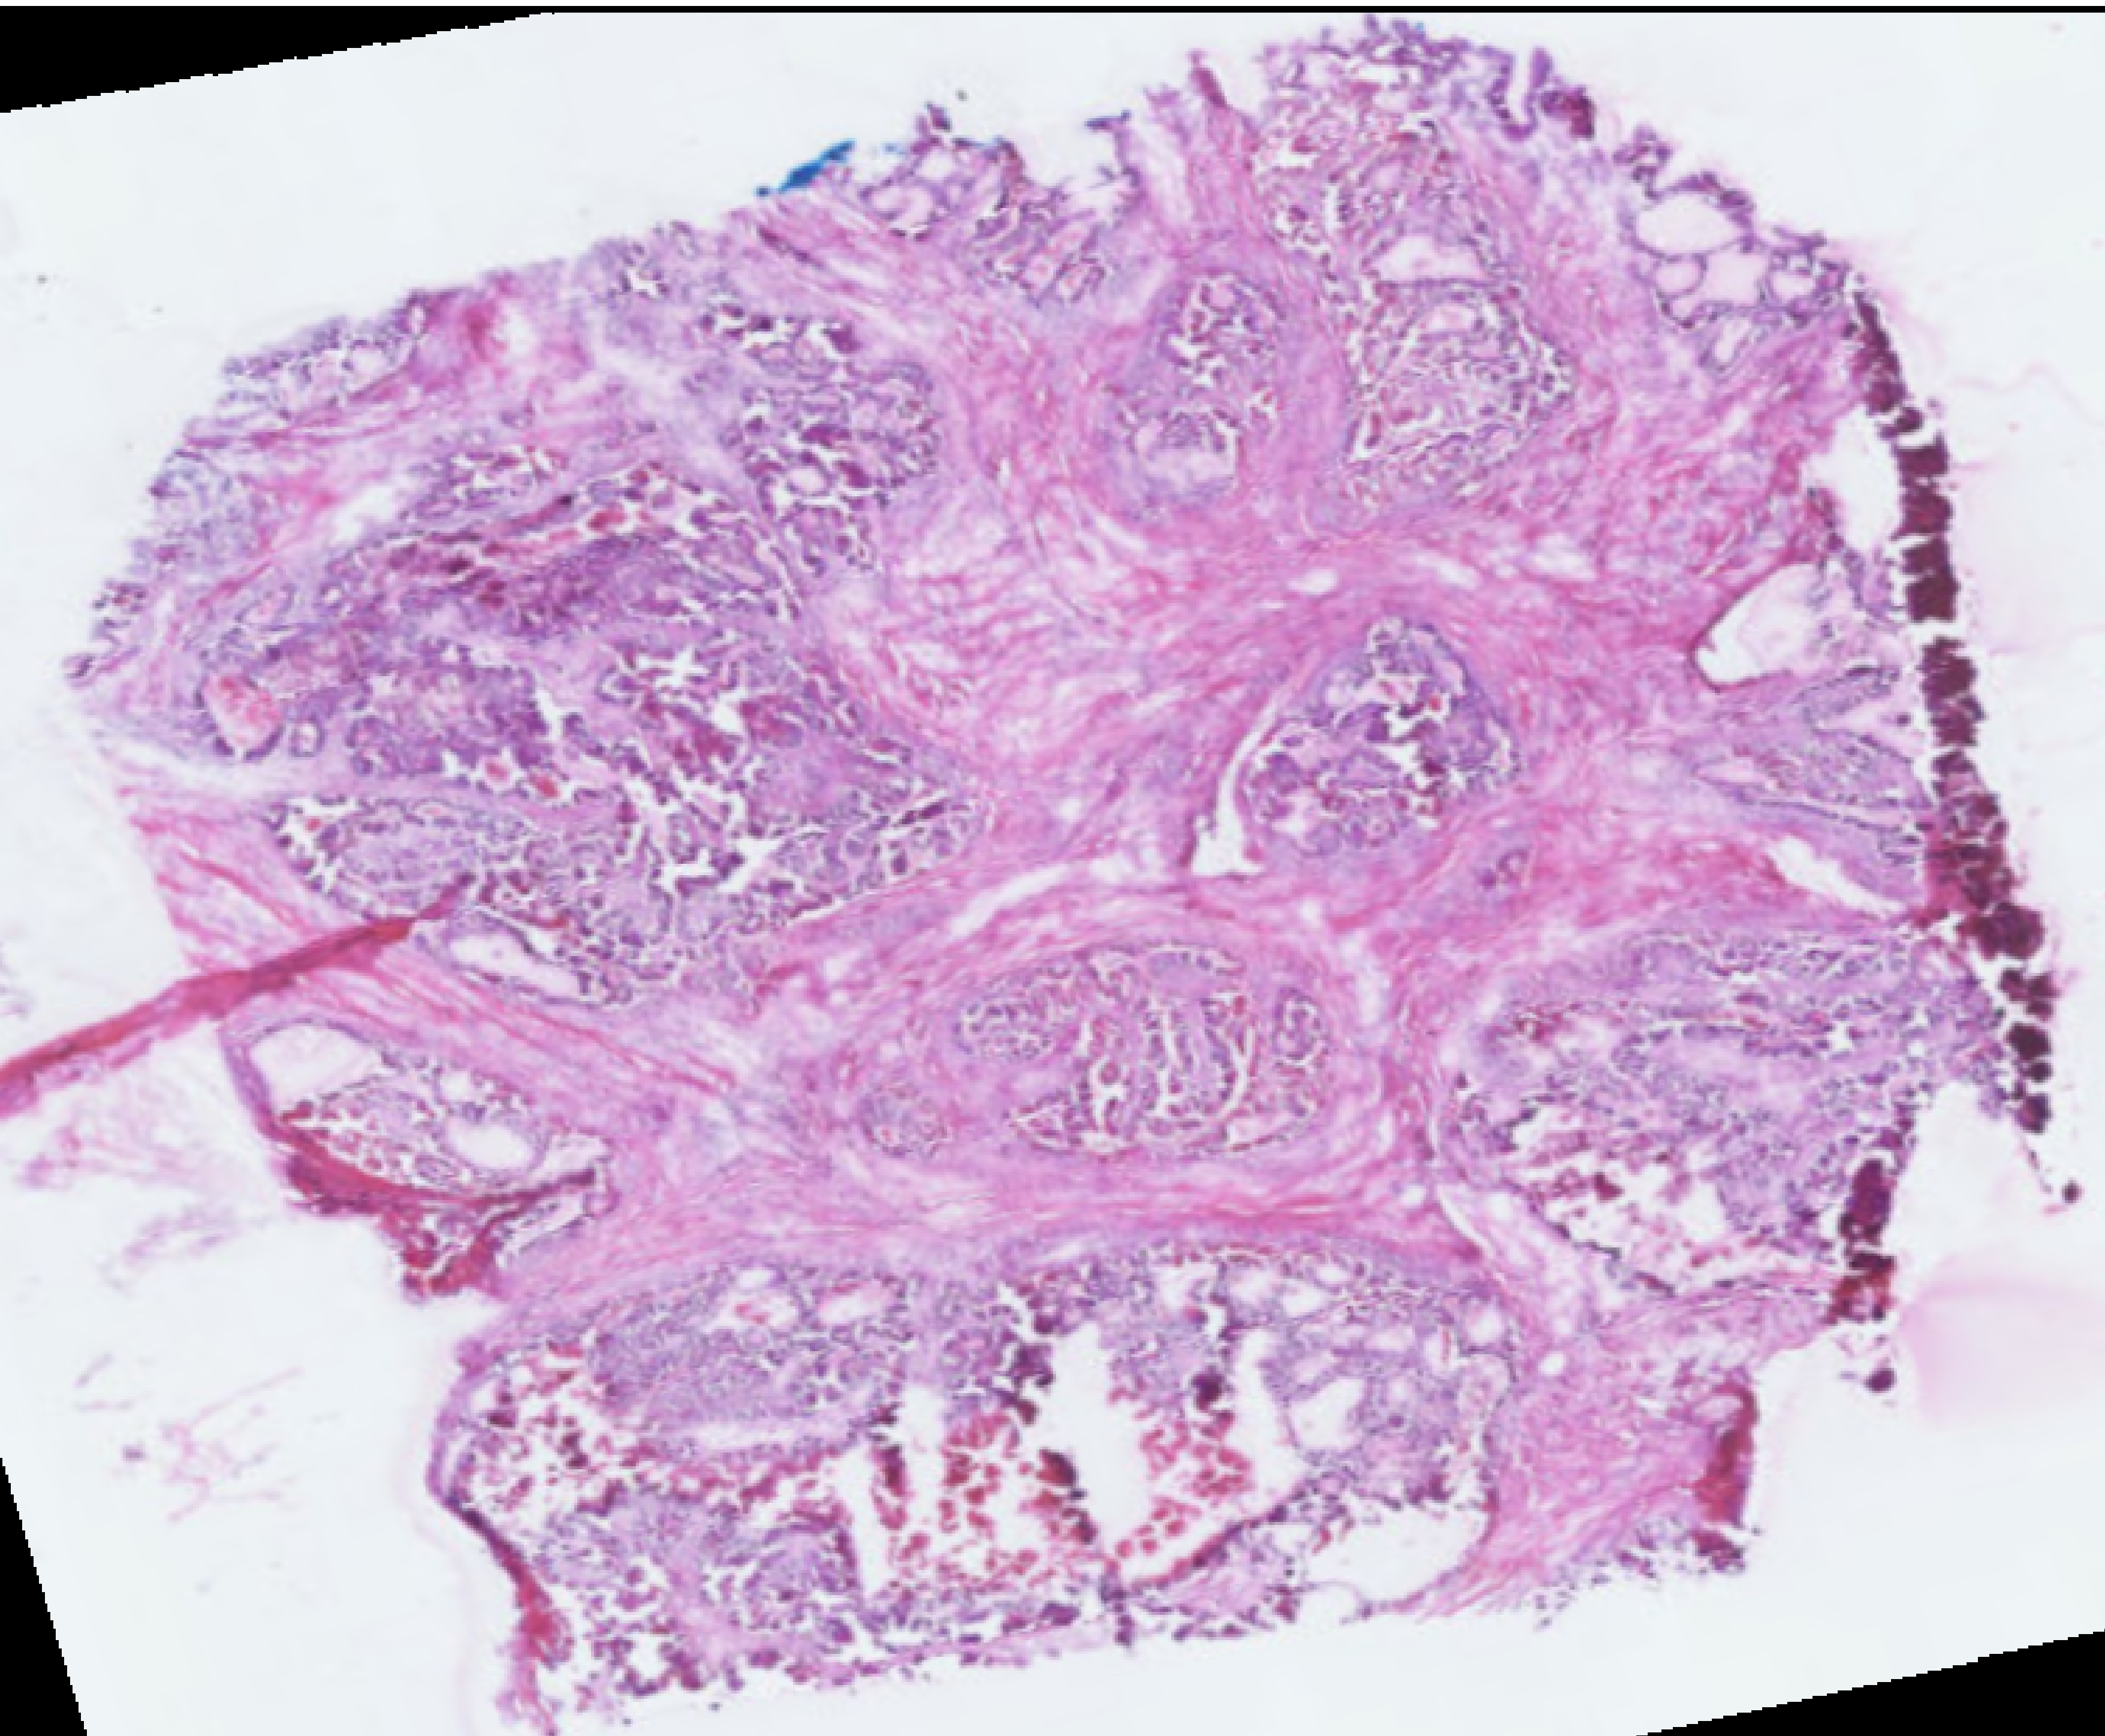
\includegraphics[width=\colWidth\textwidth]{pic/colorectal/s17_op.png}
  %   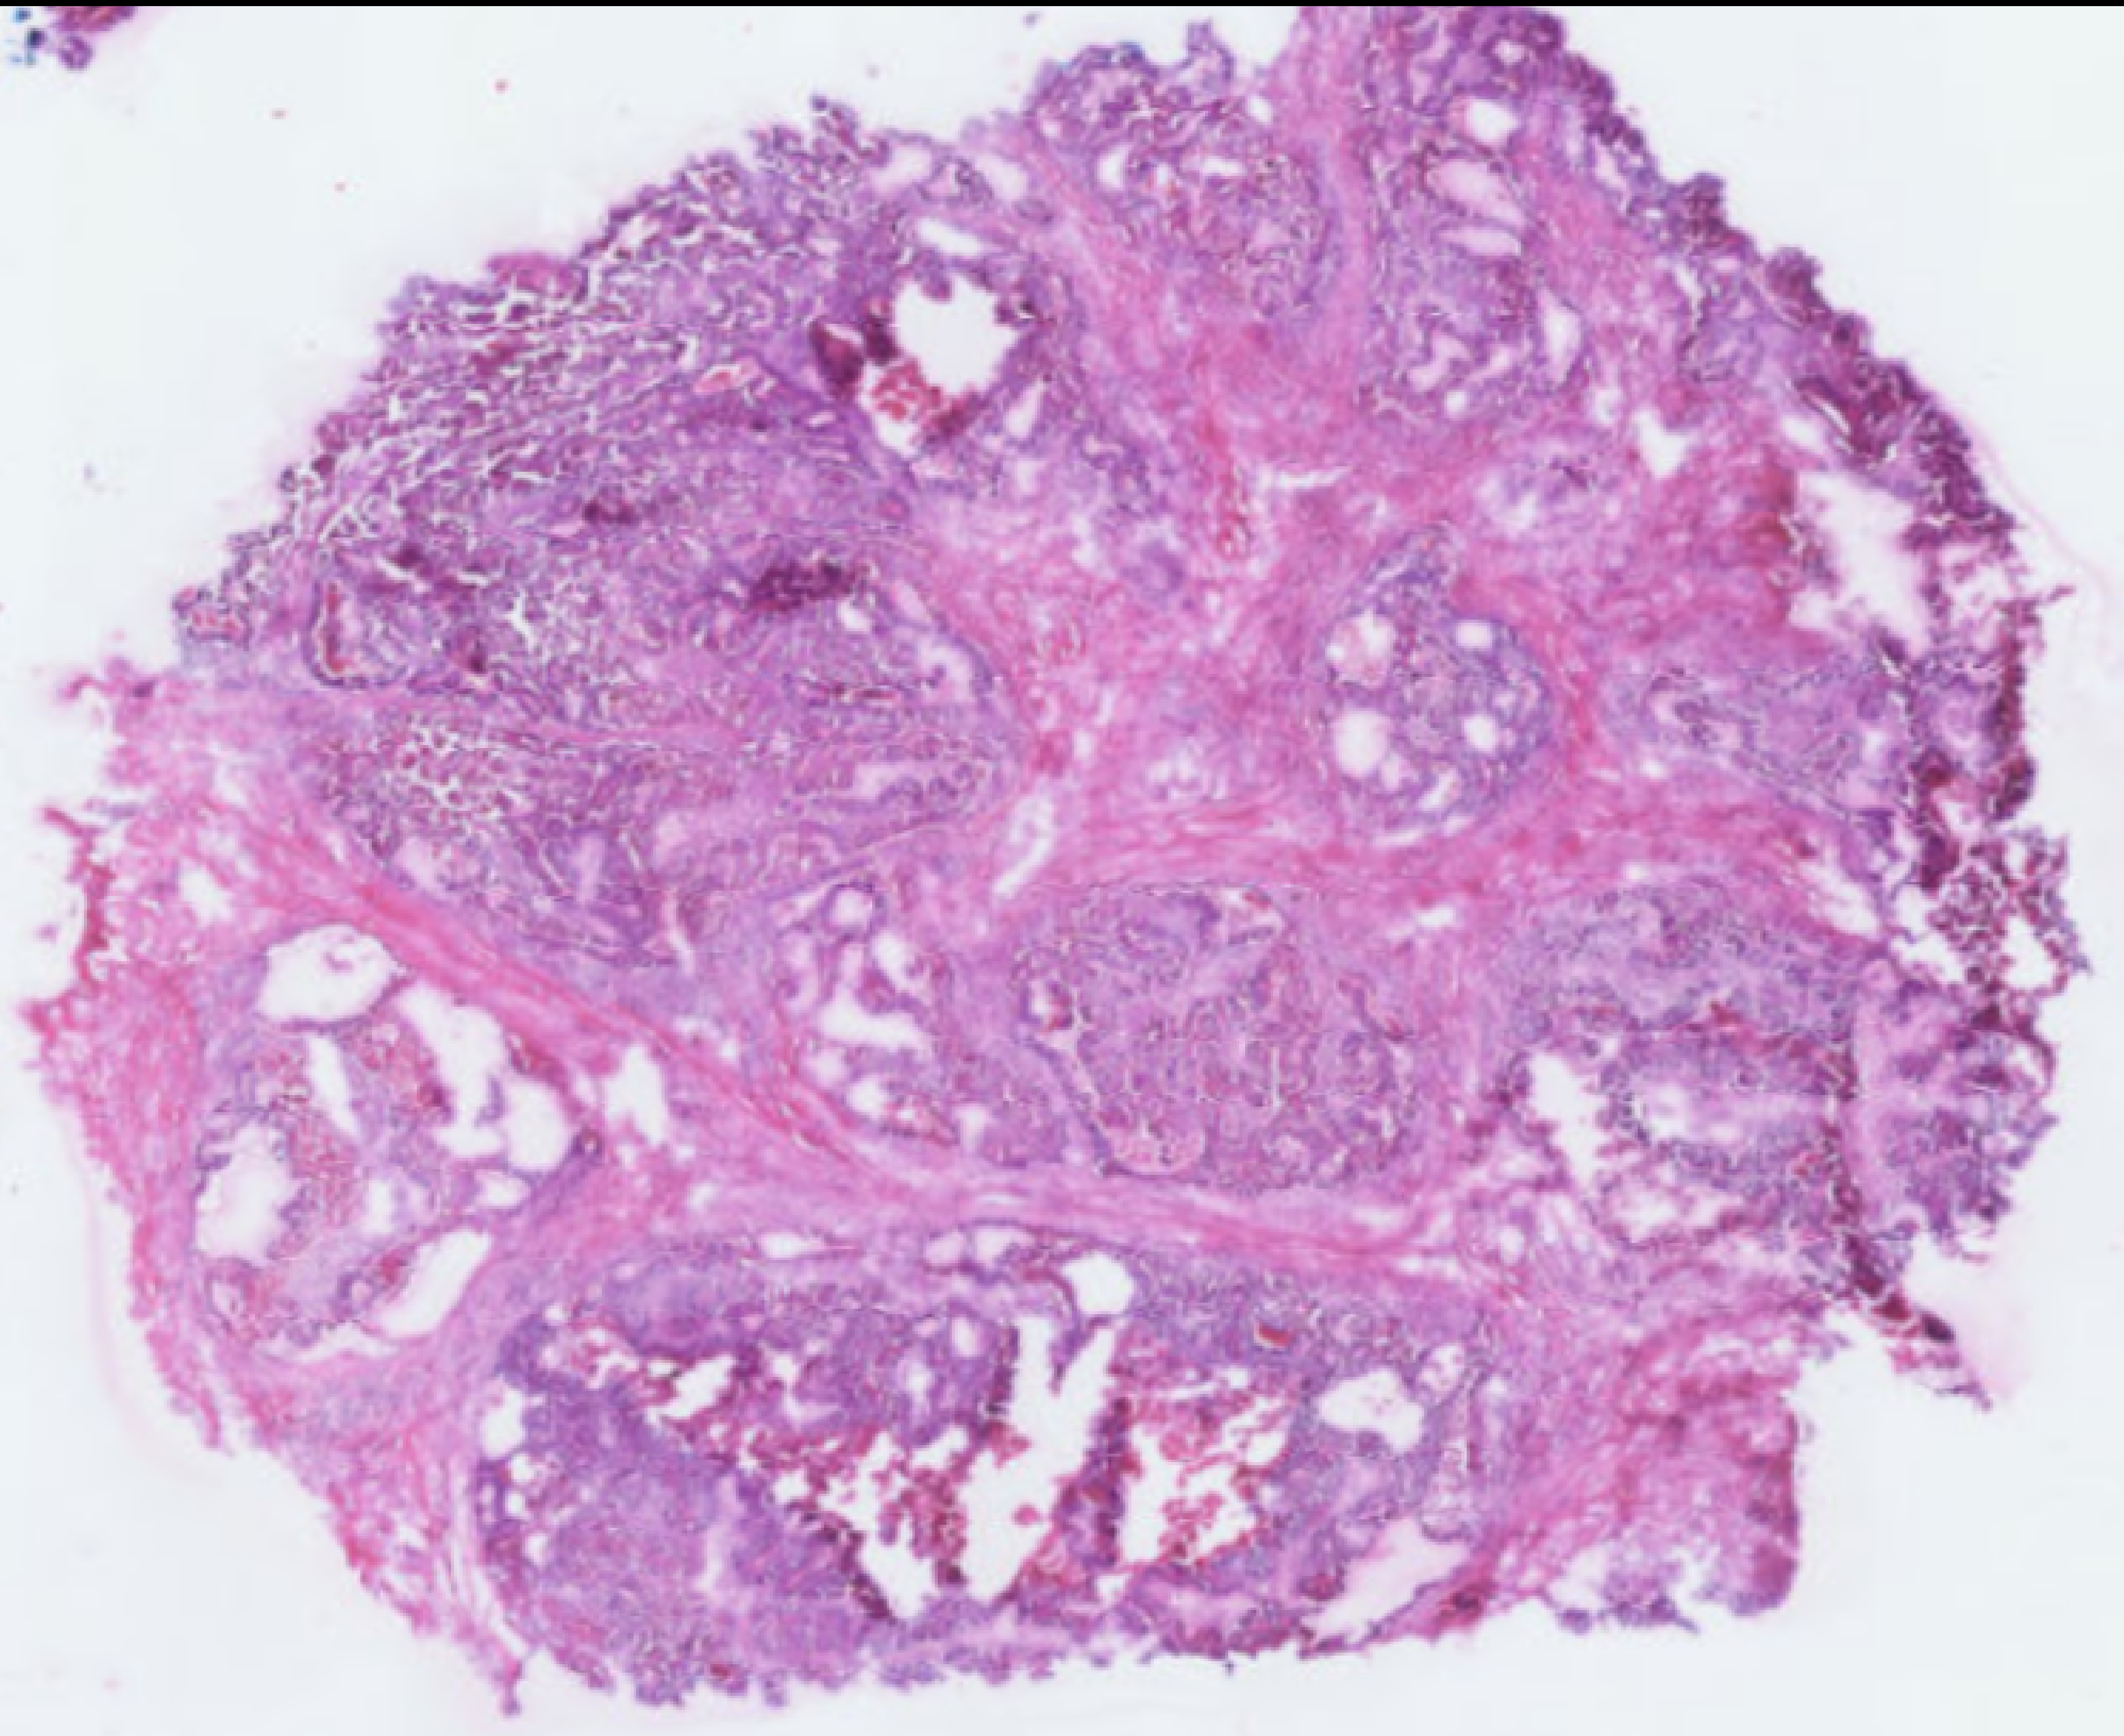
\includegraphics[width=\colWidth\textwidth]{pic/colorectal/s18_op.png}
  %   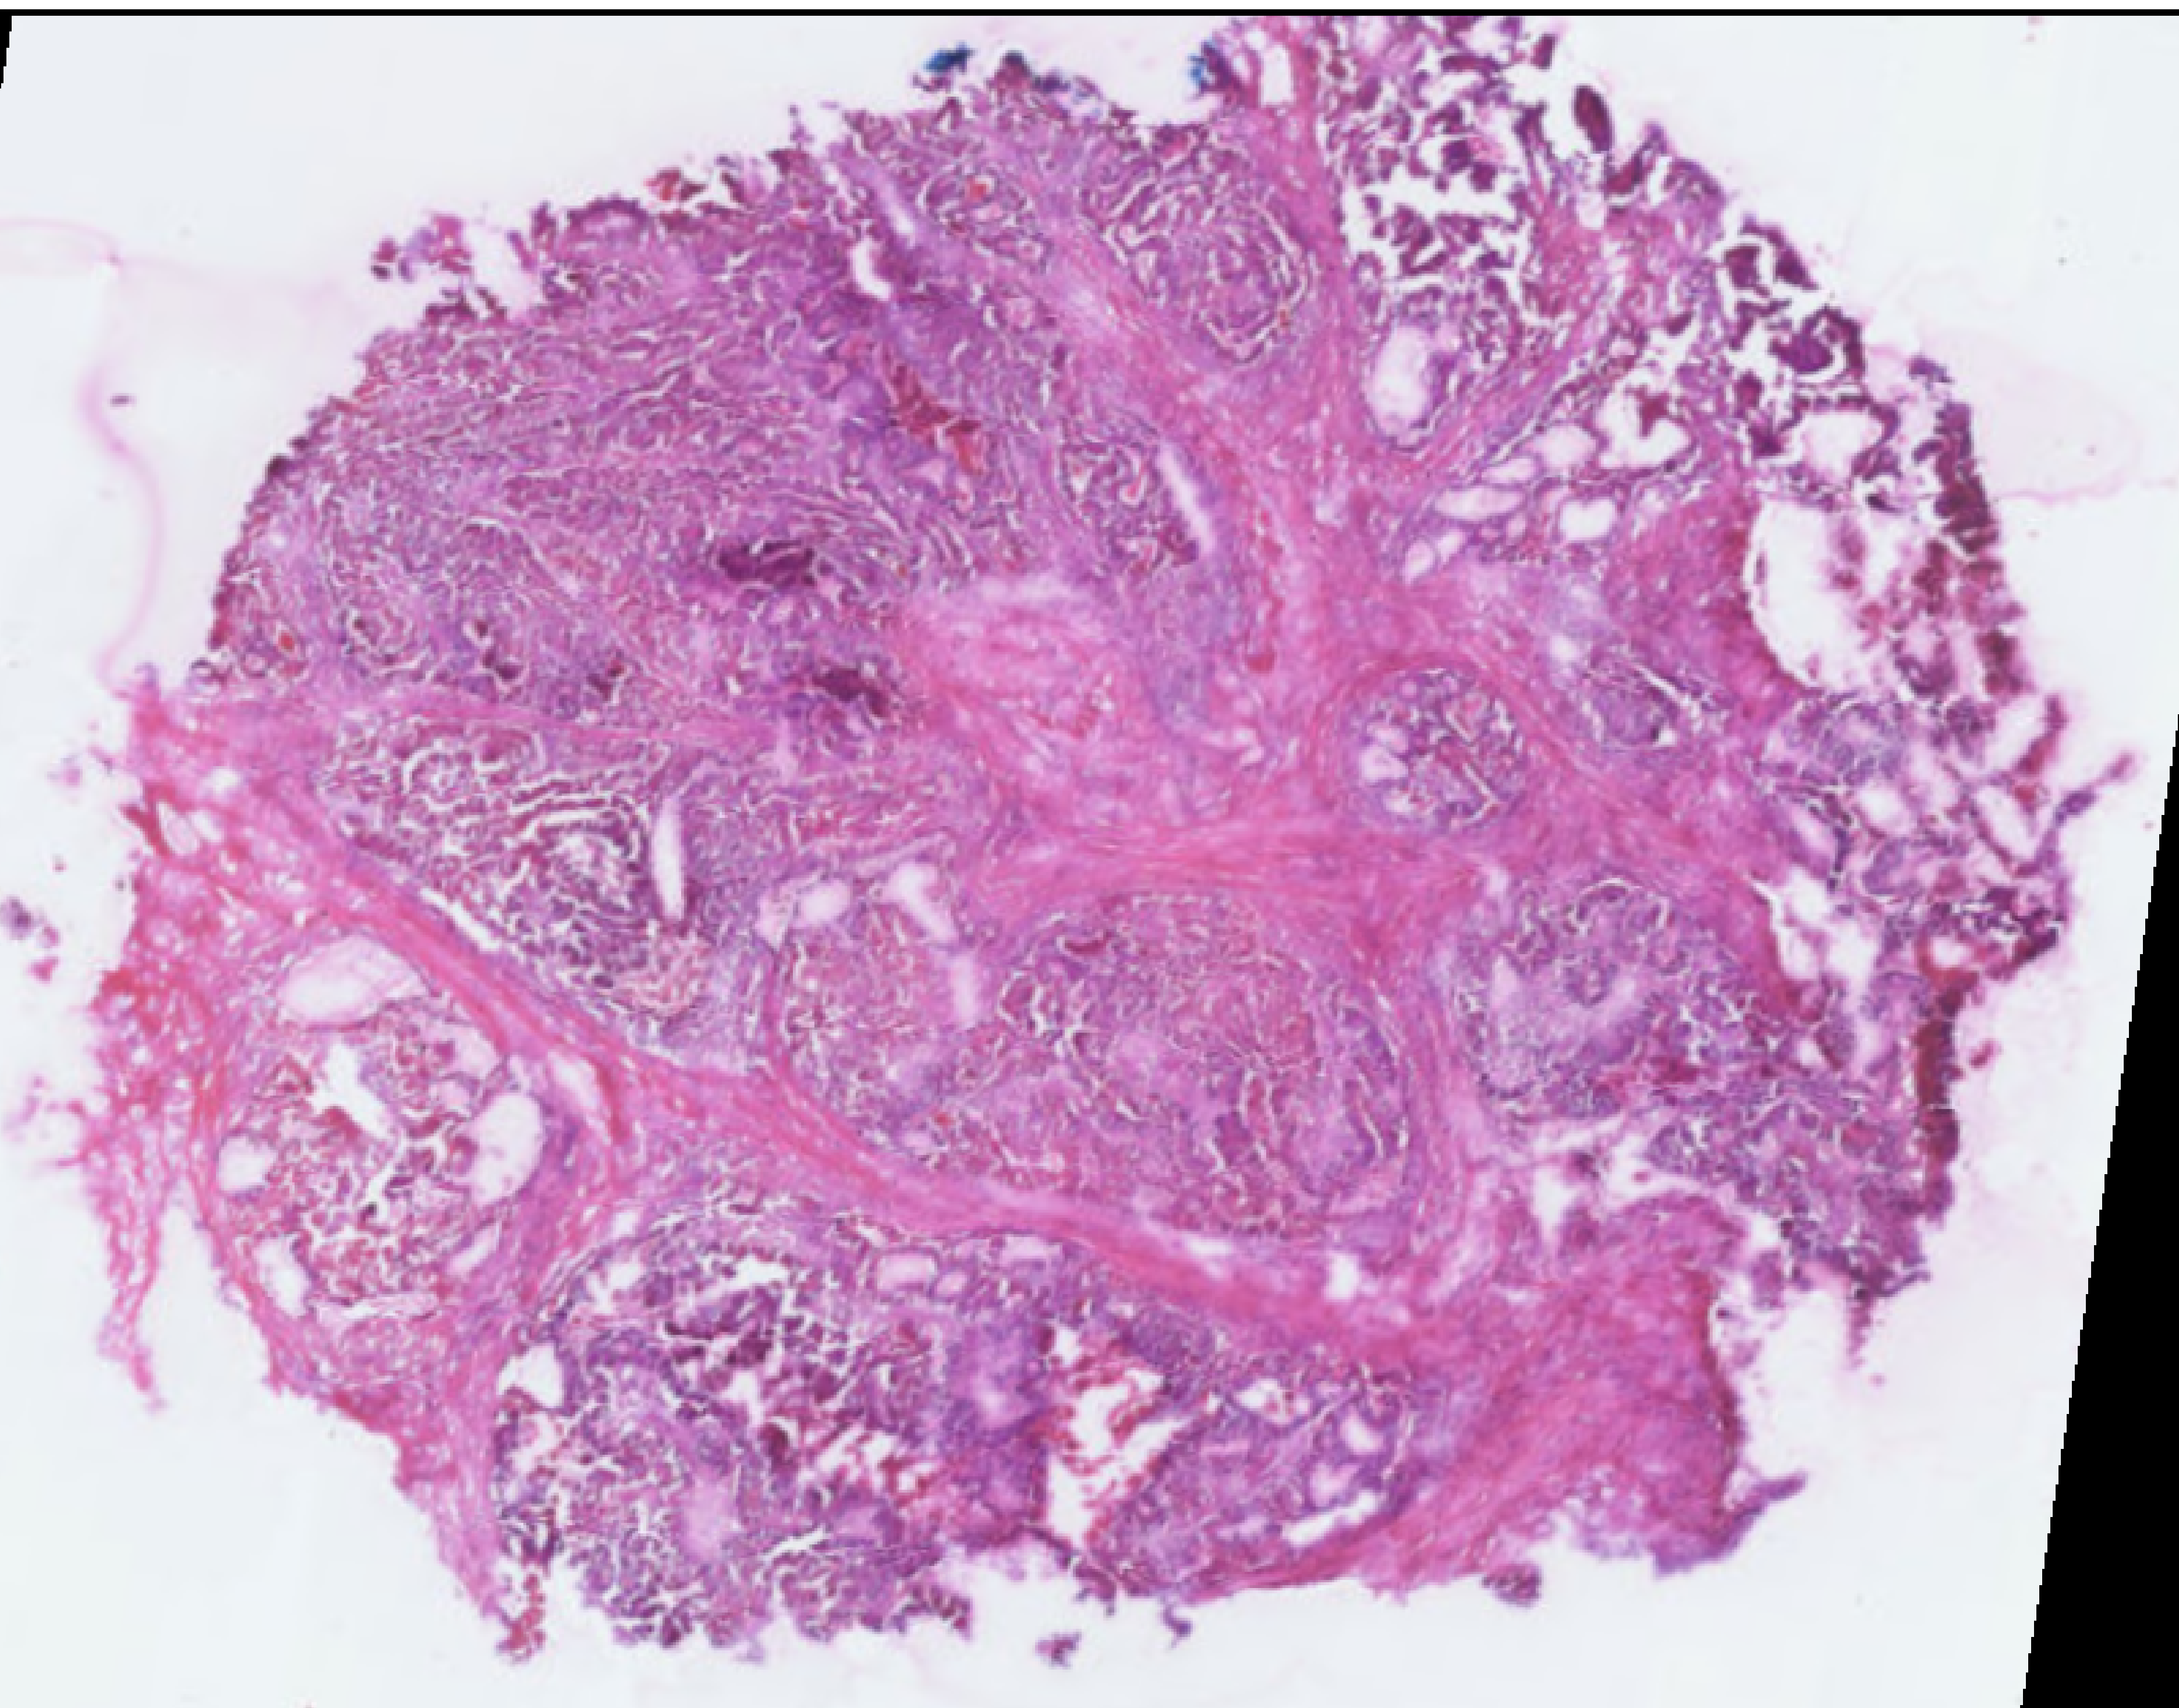
\includegraphics[width=\colWidth\textwidth]{pic/colorectal/s19_op.png}
  %   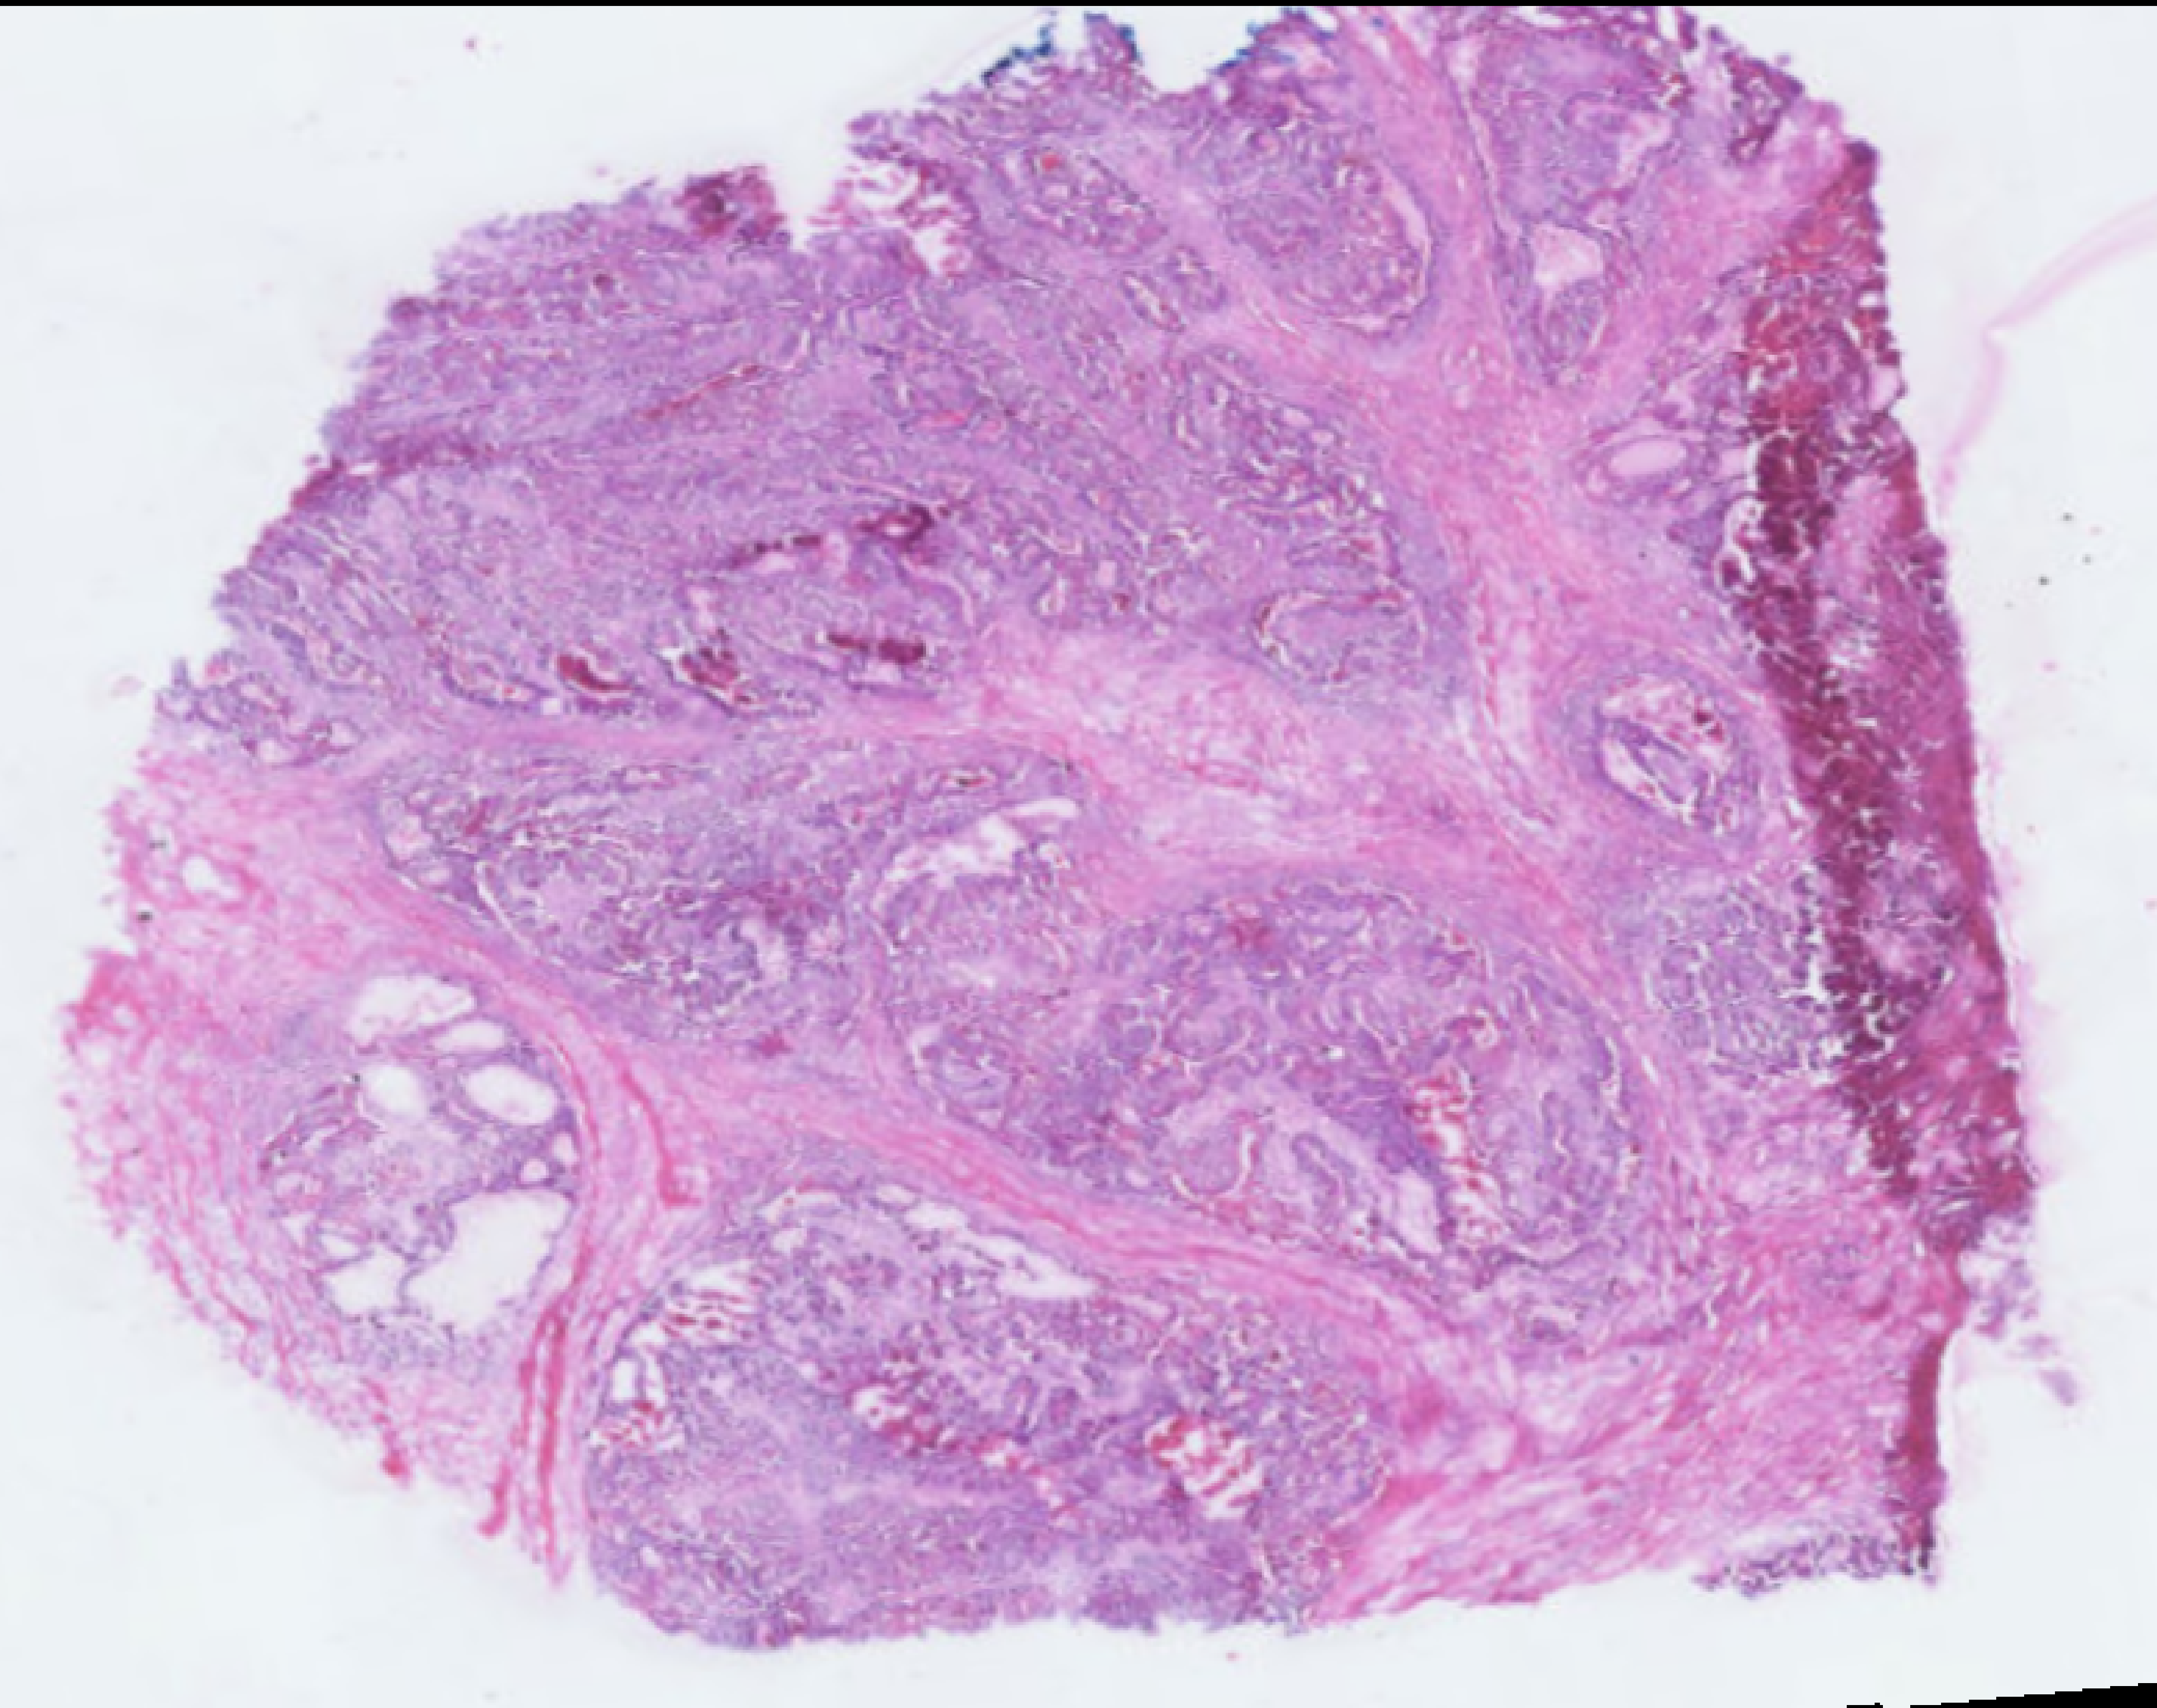
\includegraphics[width=\colWidth\textwidth]{pic/colorectal/s20_op.png}
  %   \\
  %   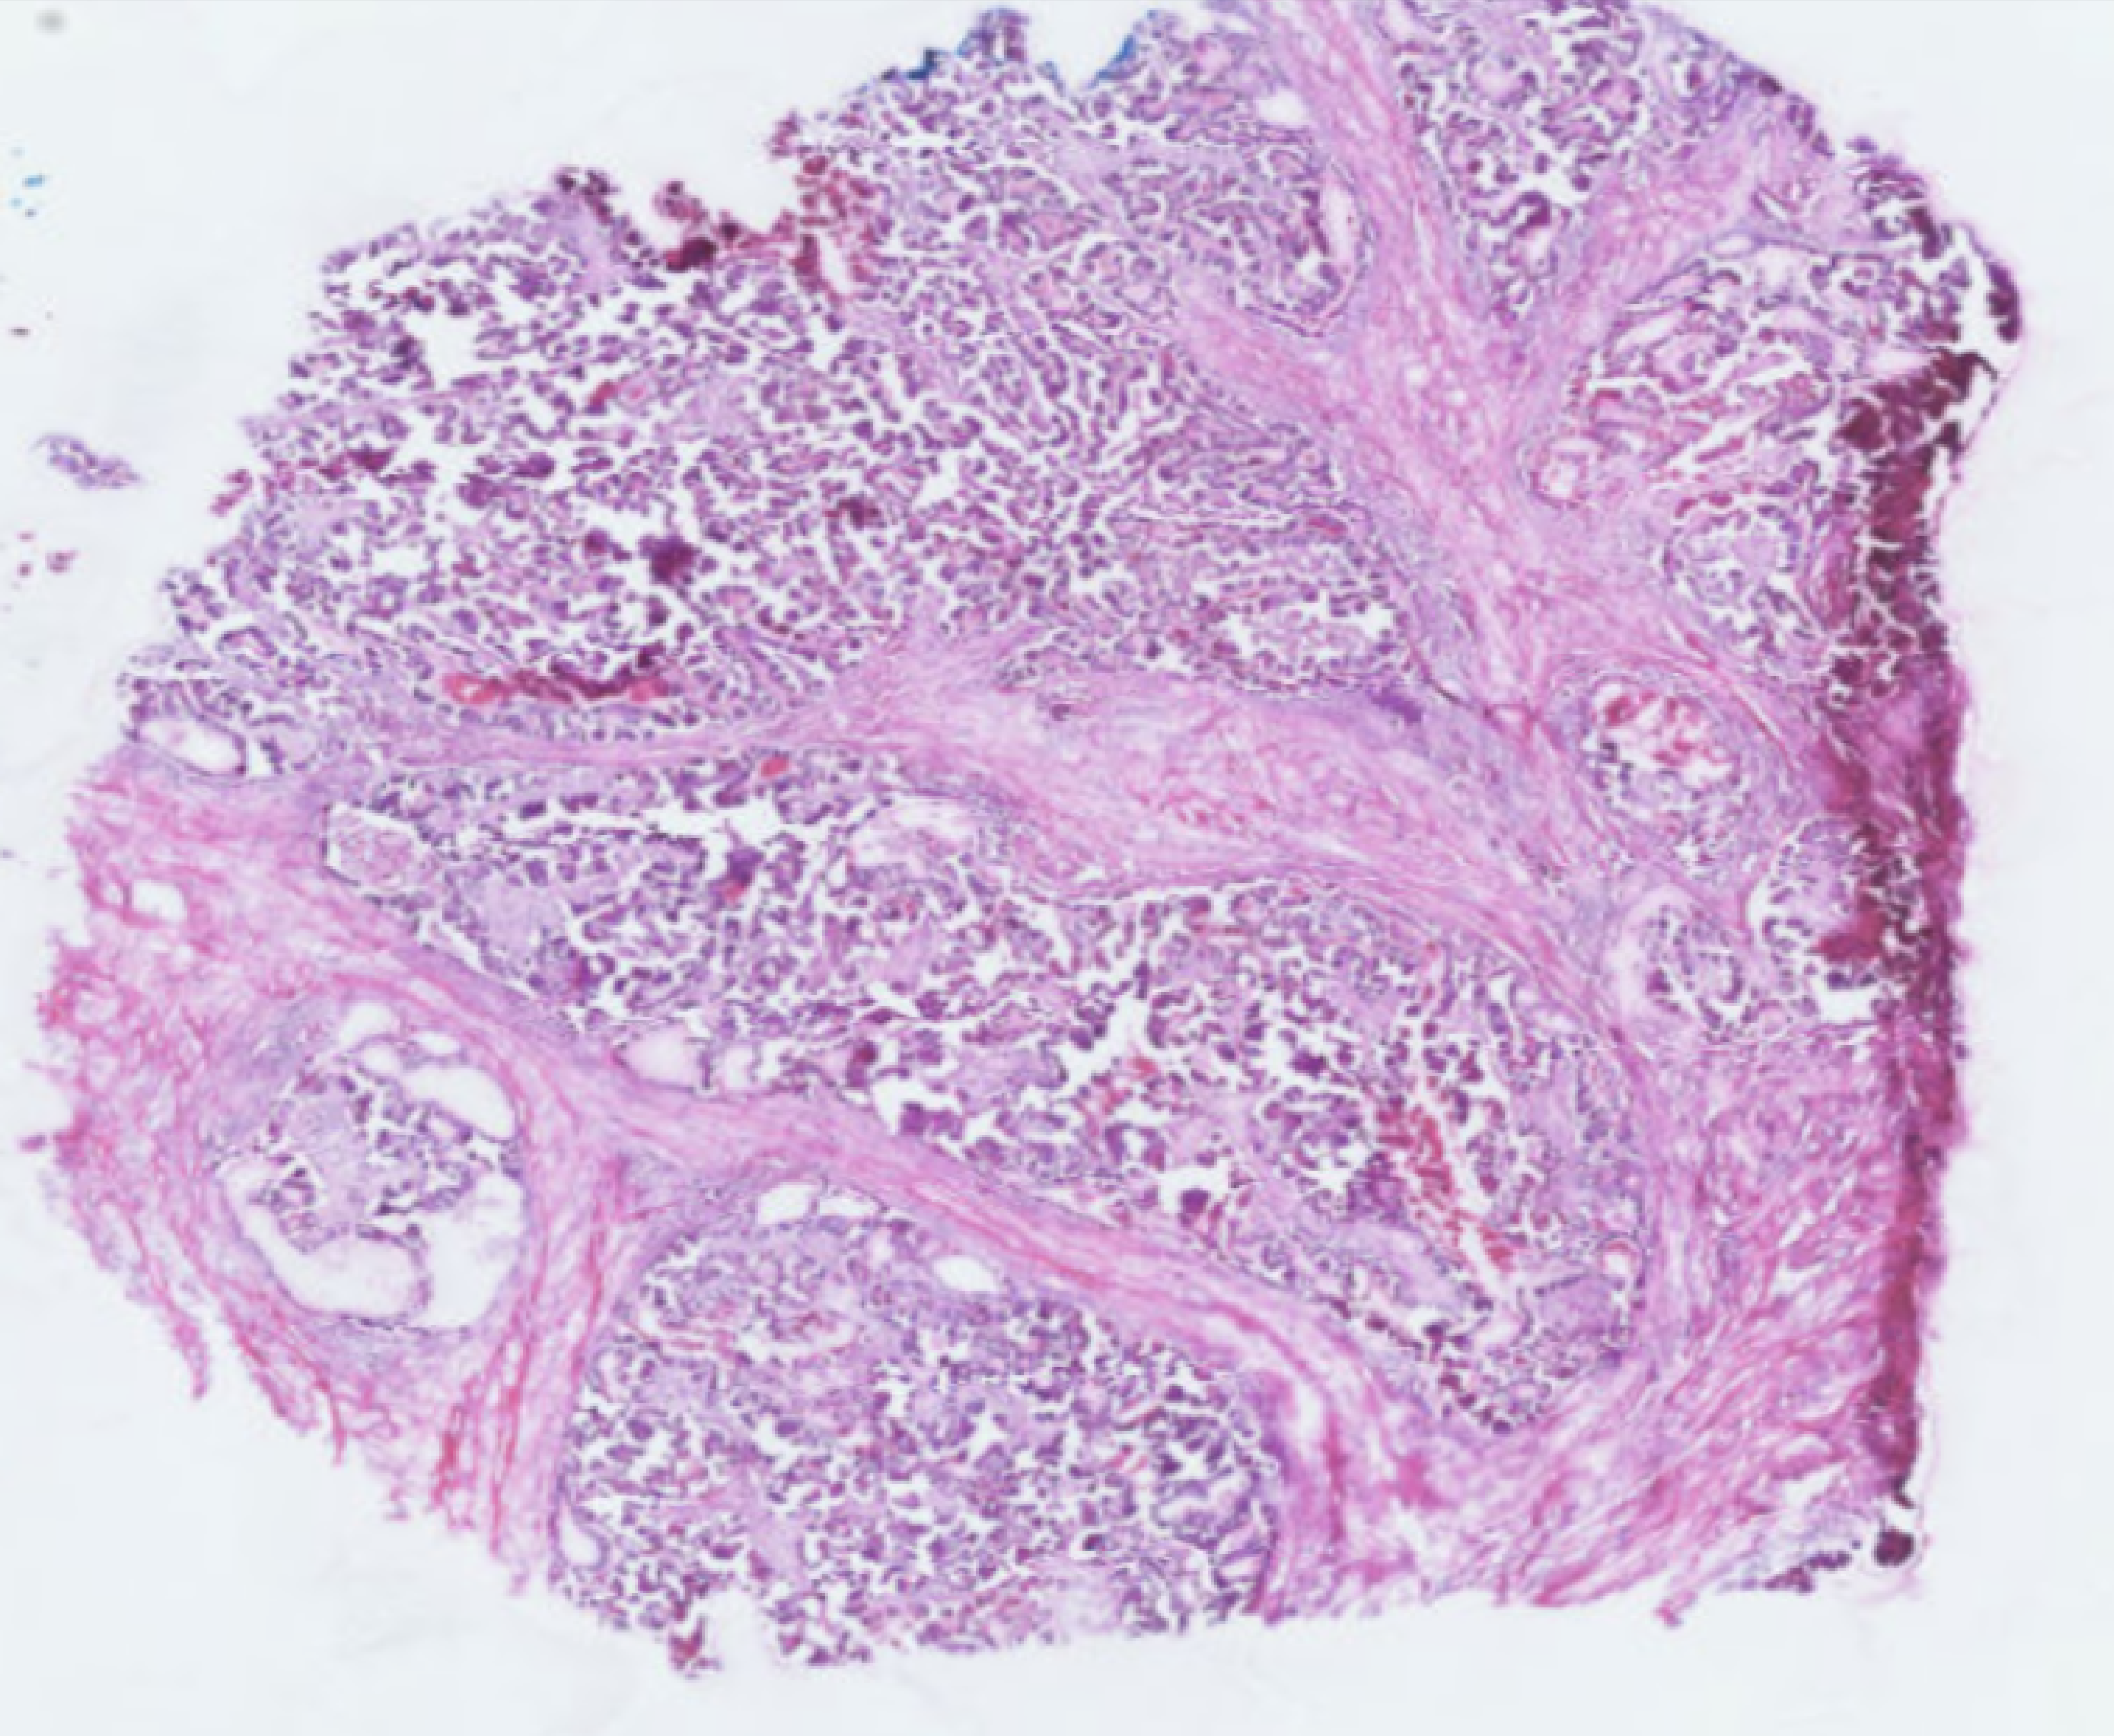
\includegraphics[width=\colWidth\textwidth]{pic/colorectal/s21_op.png}
  %   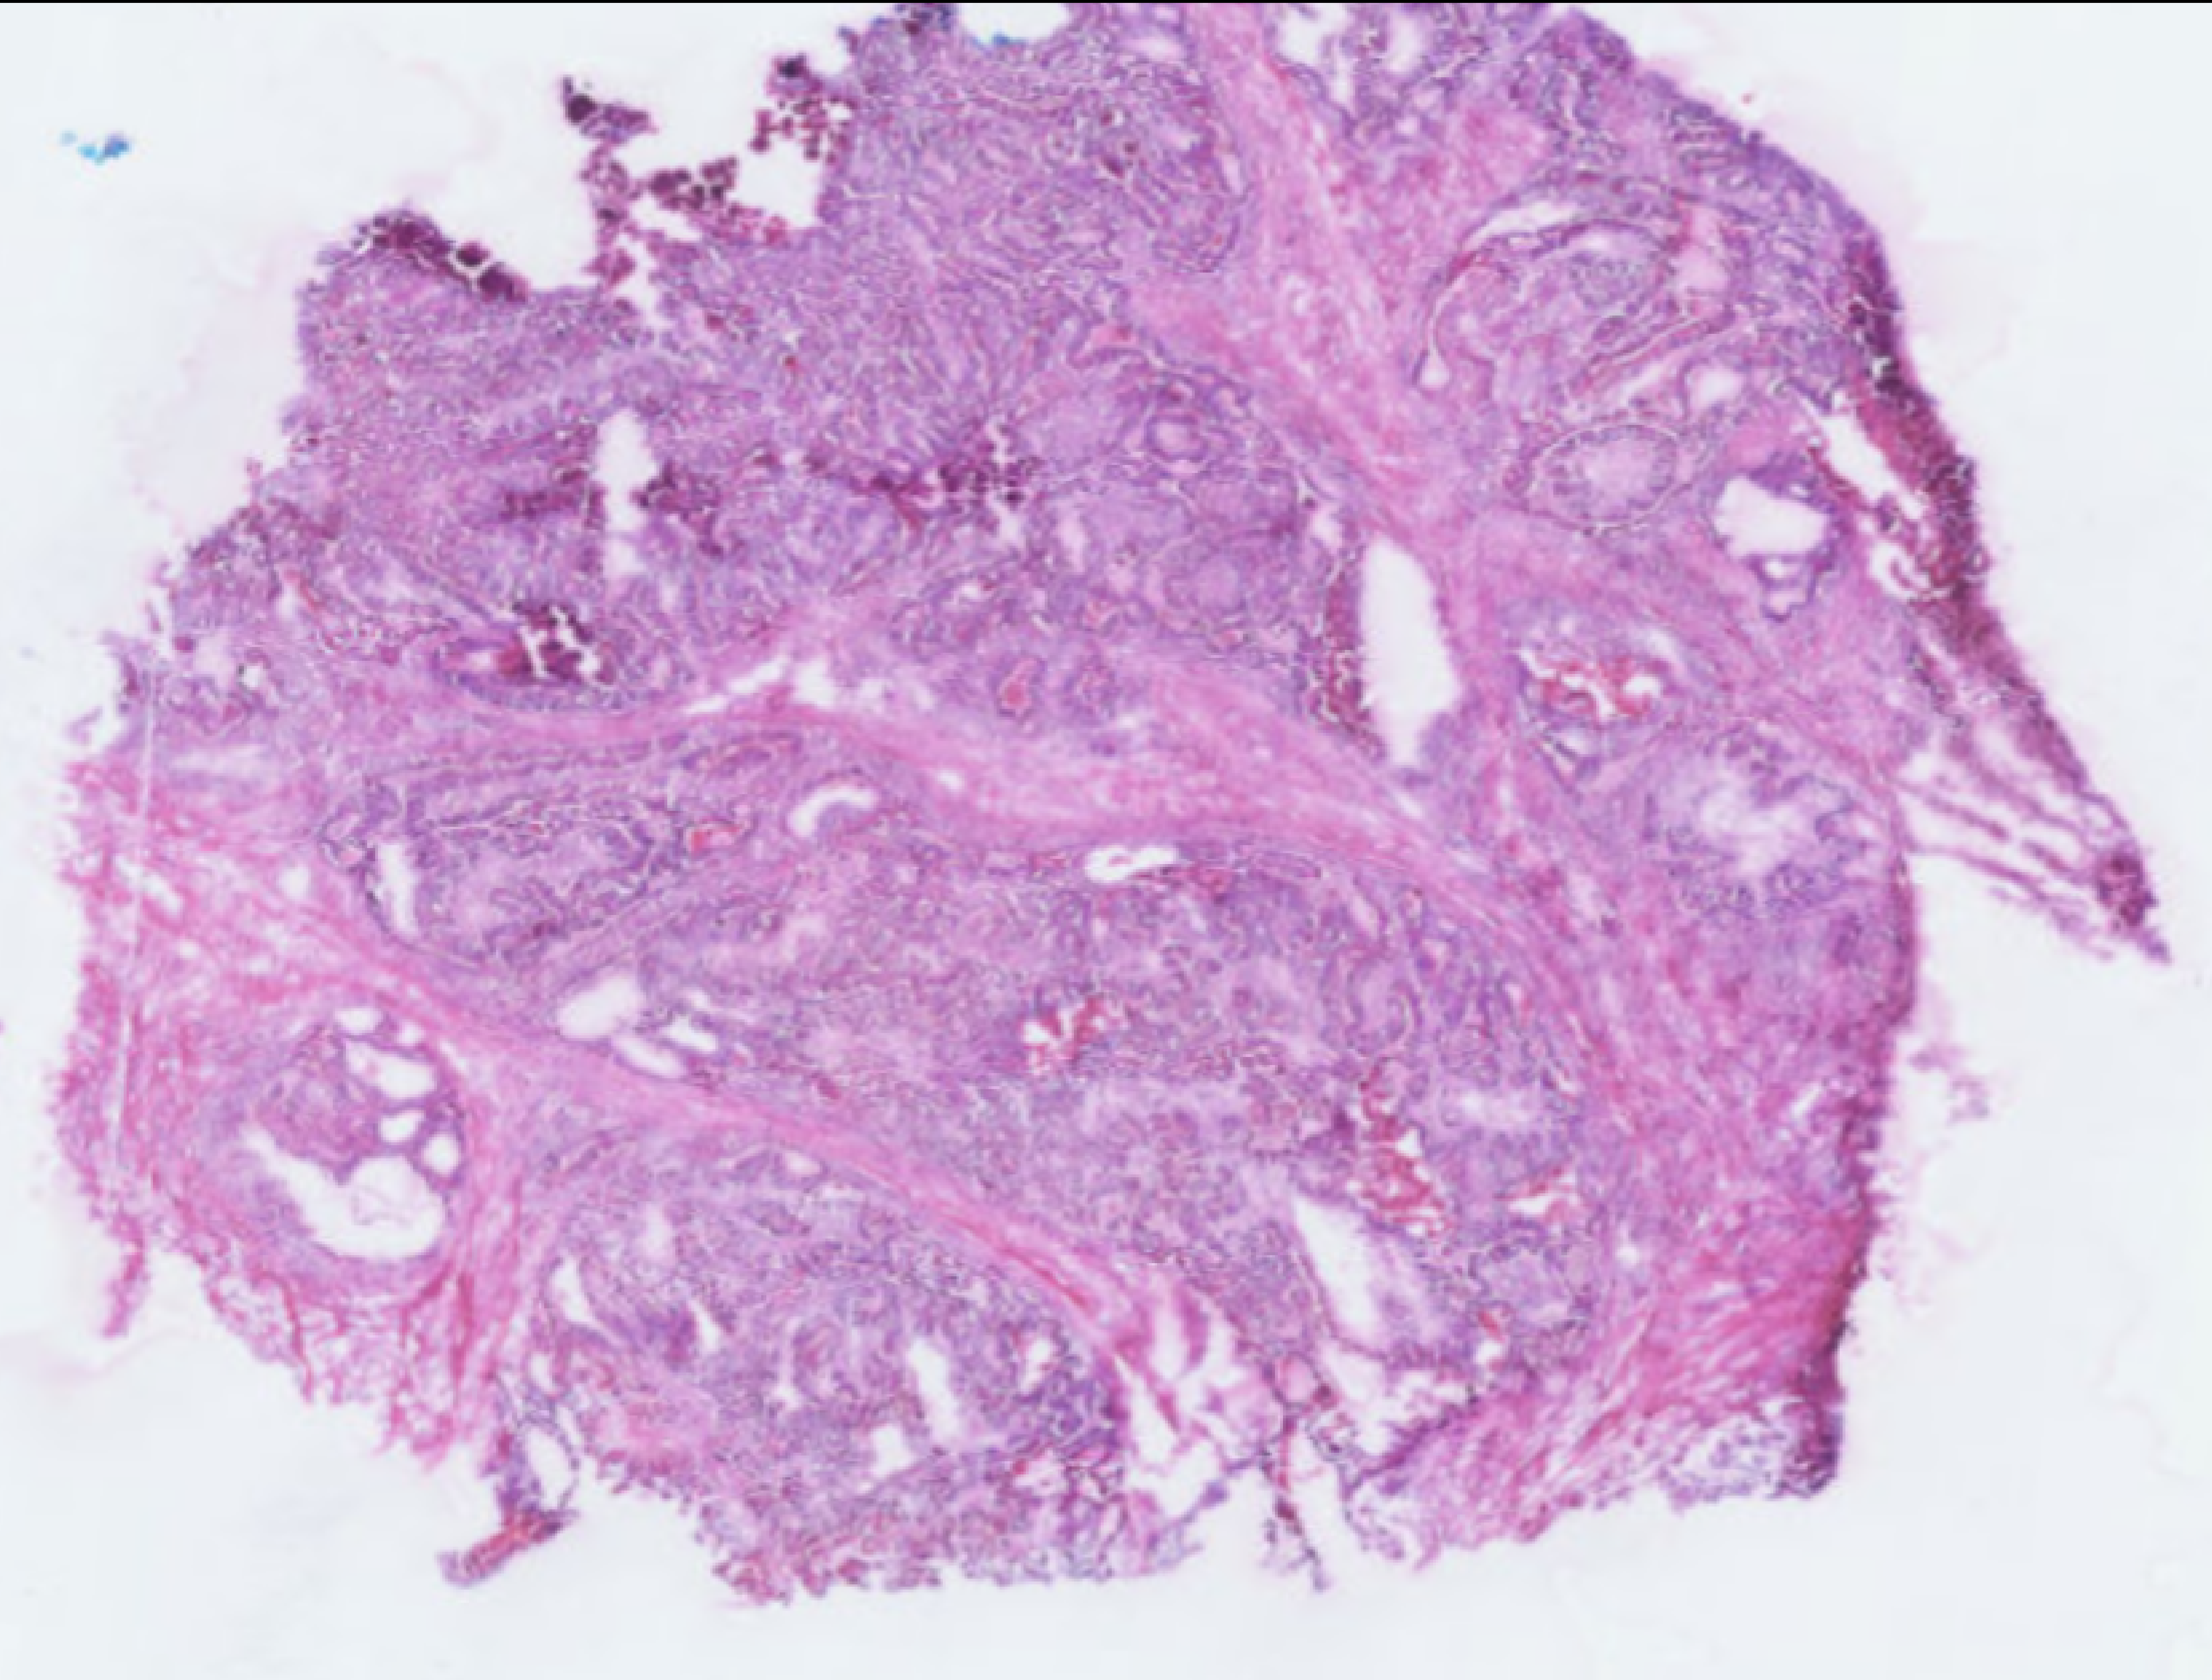
\includegraphics[width=\colWidth\textwidth]{pic/colorectal/s22_op.png}
  %   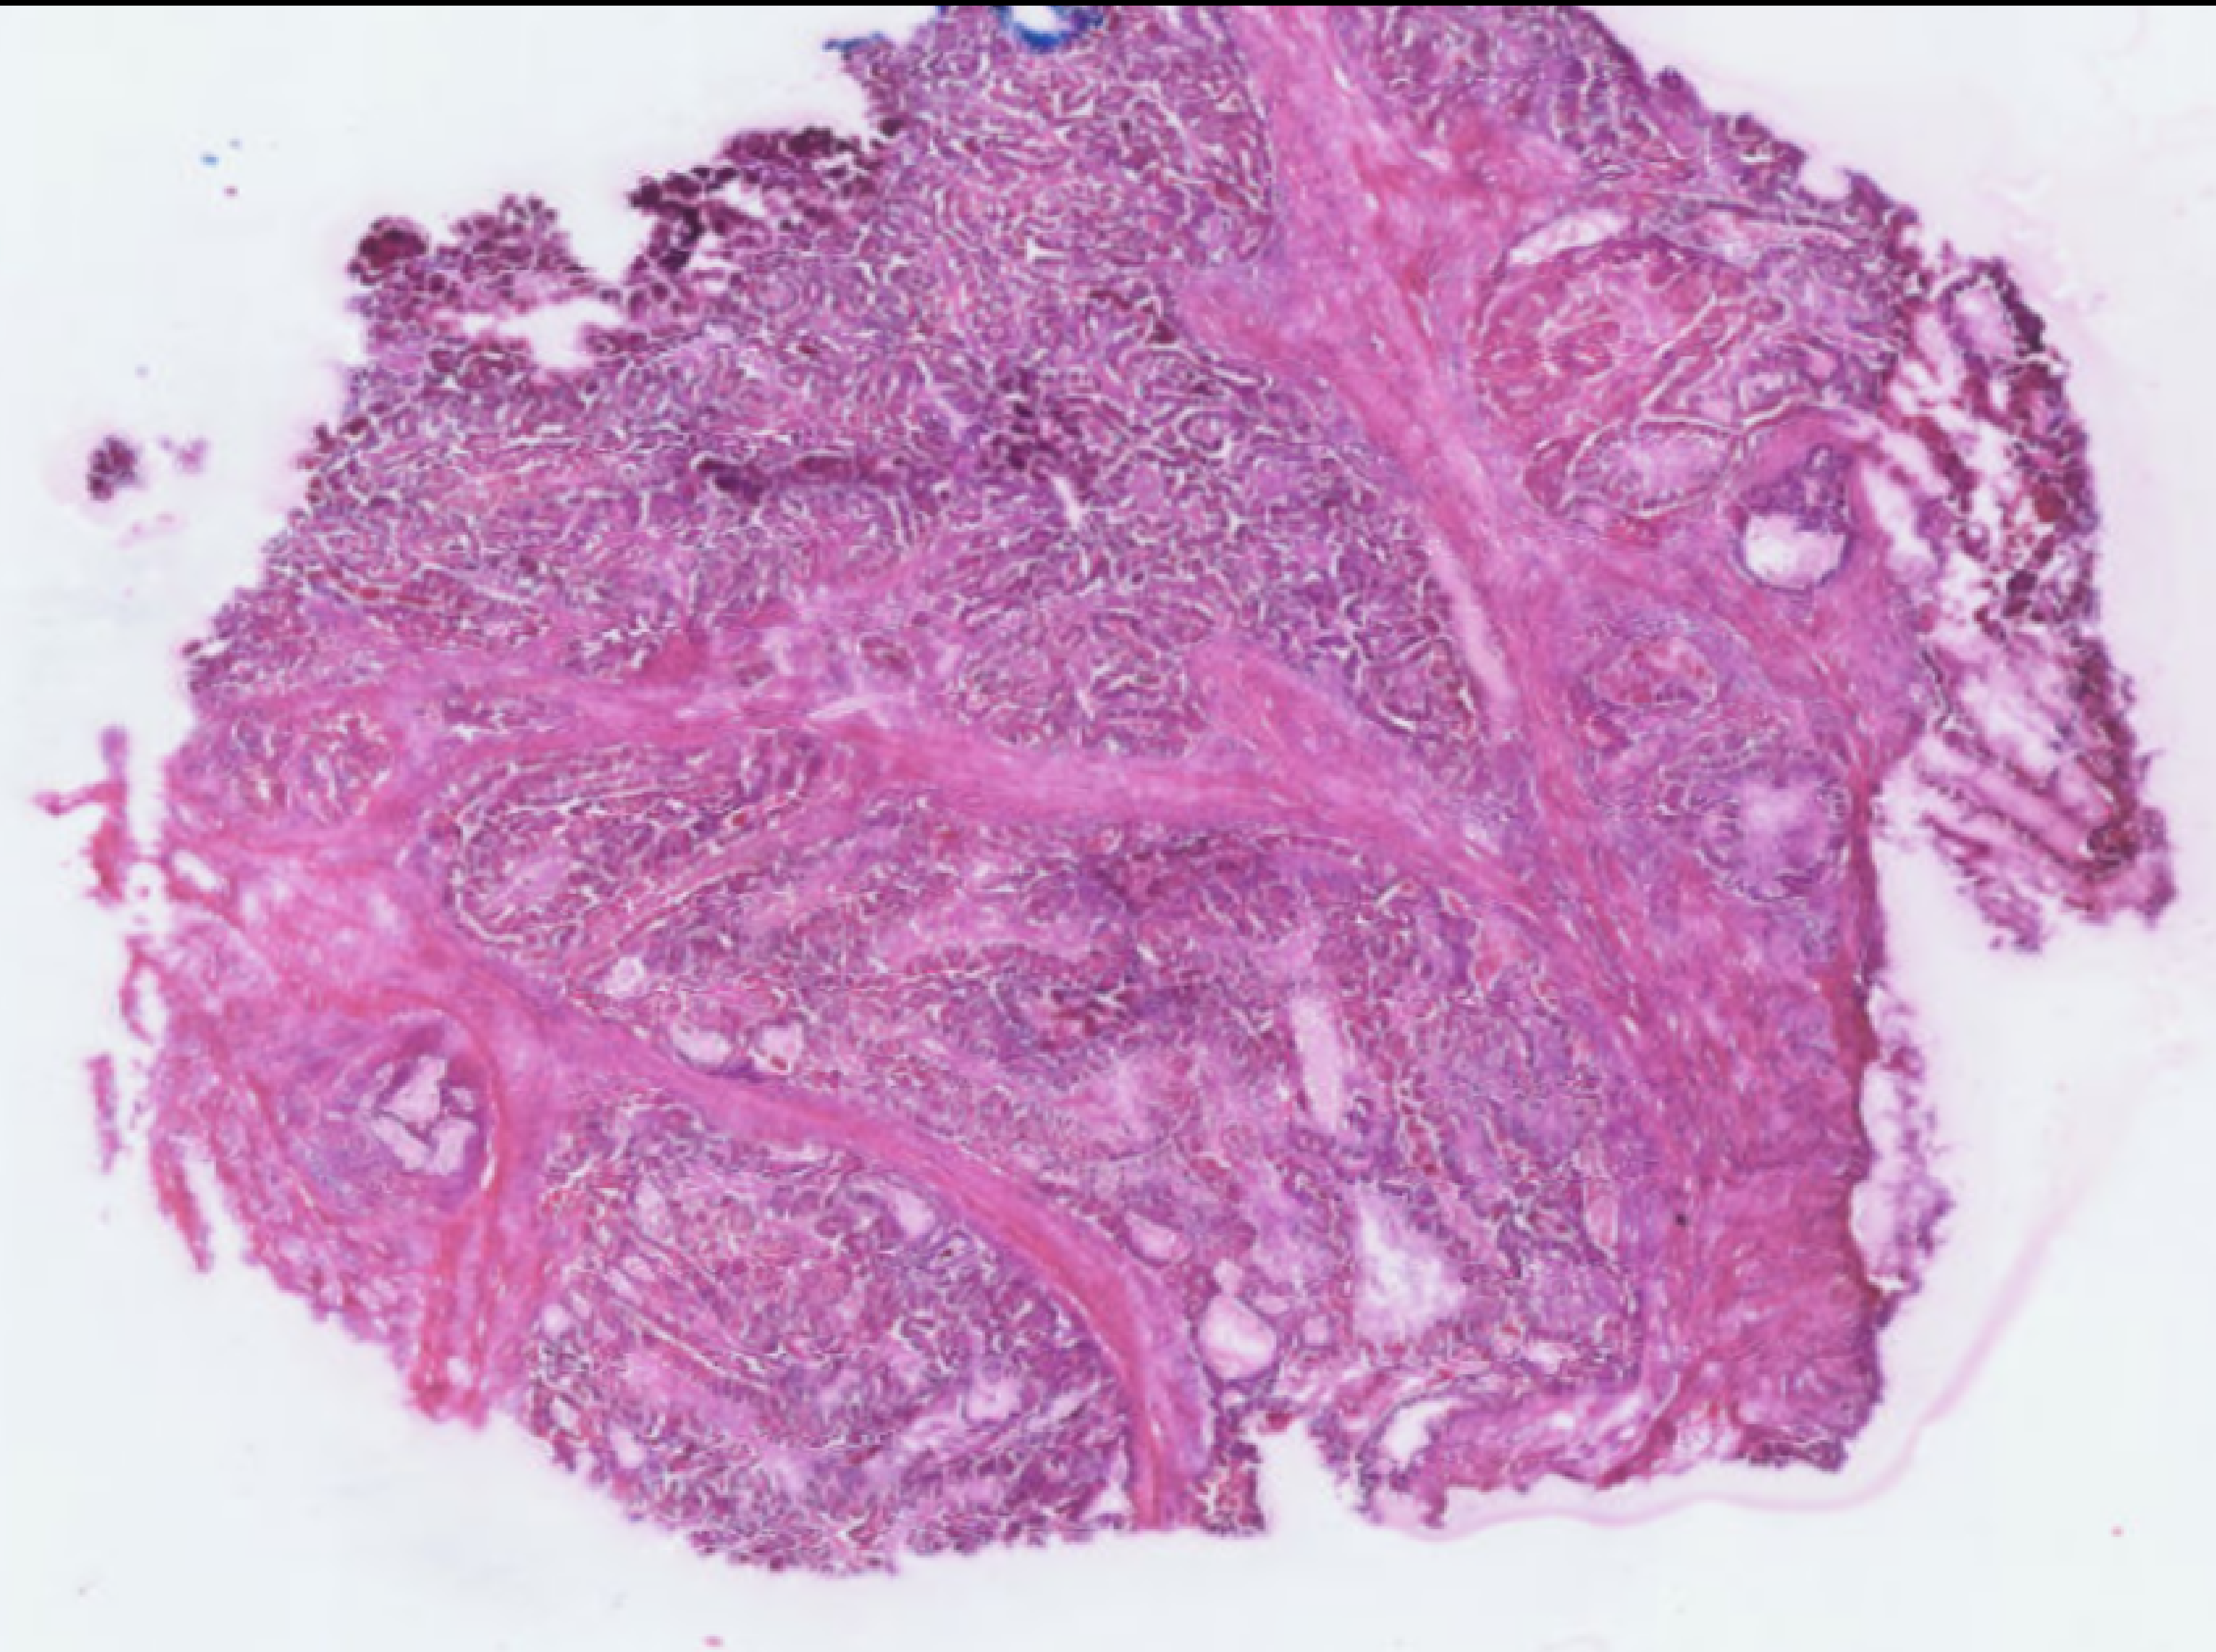
\includegraphics[width=\colWidth\textwidth]{pic/colorectal/s23_op.png}
  %   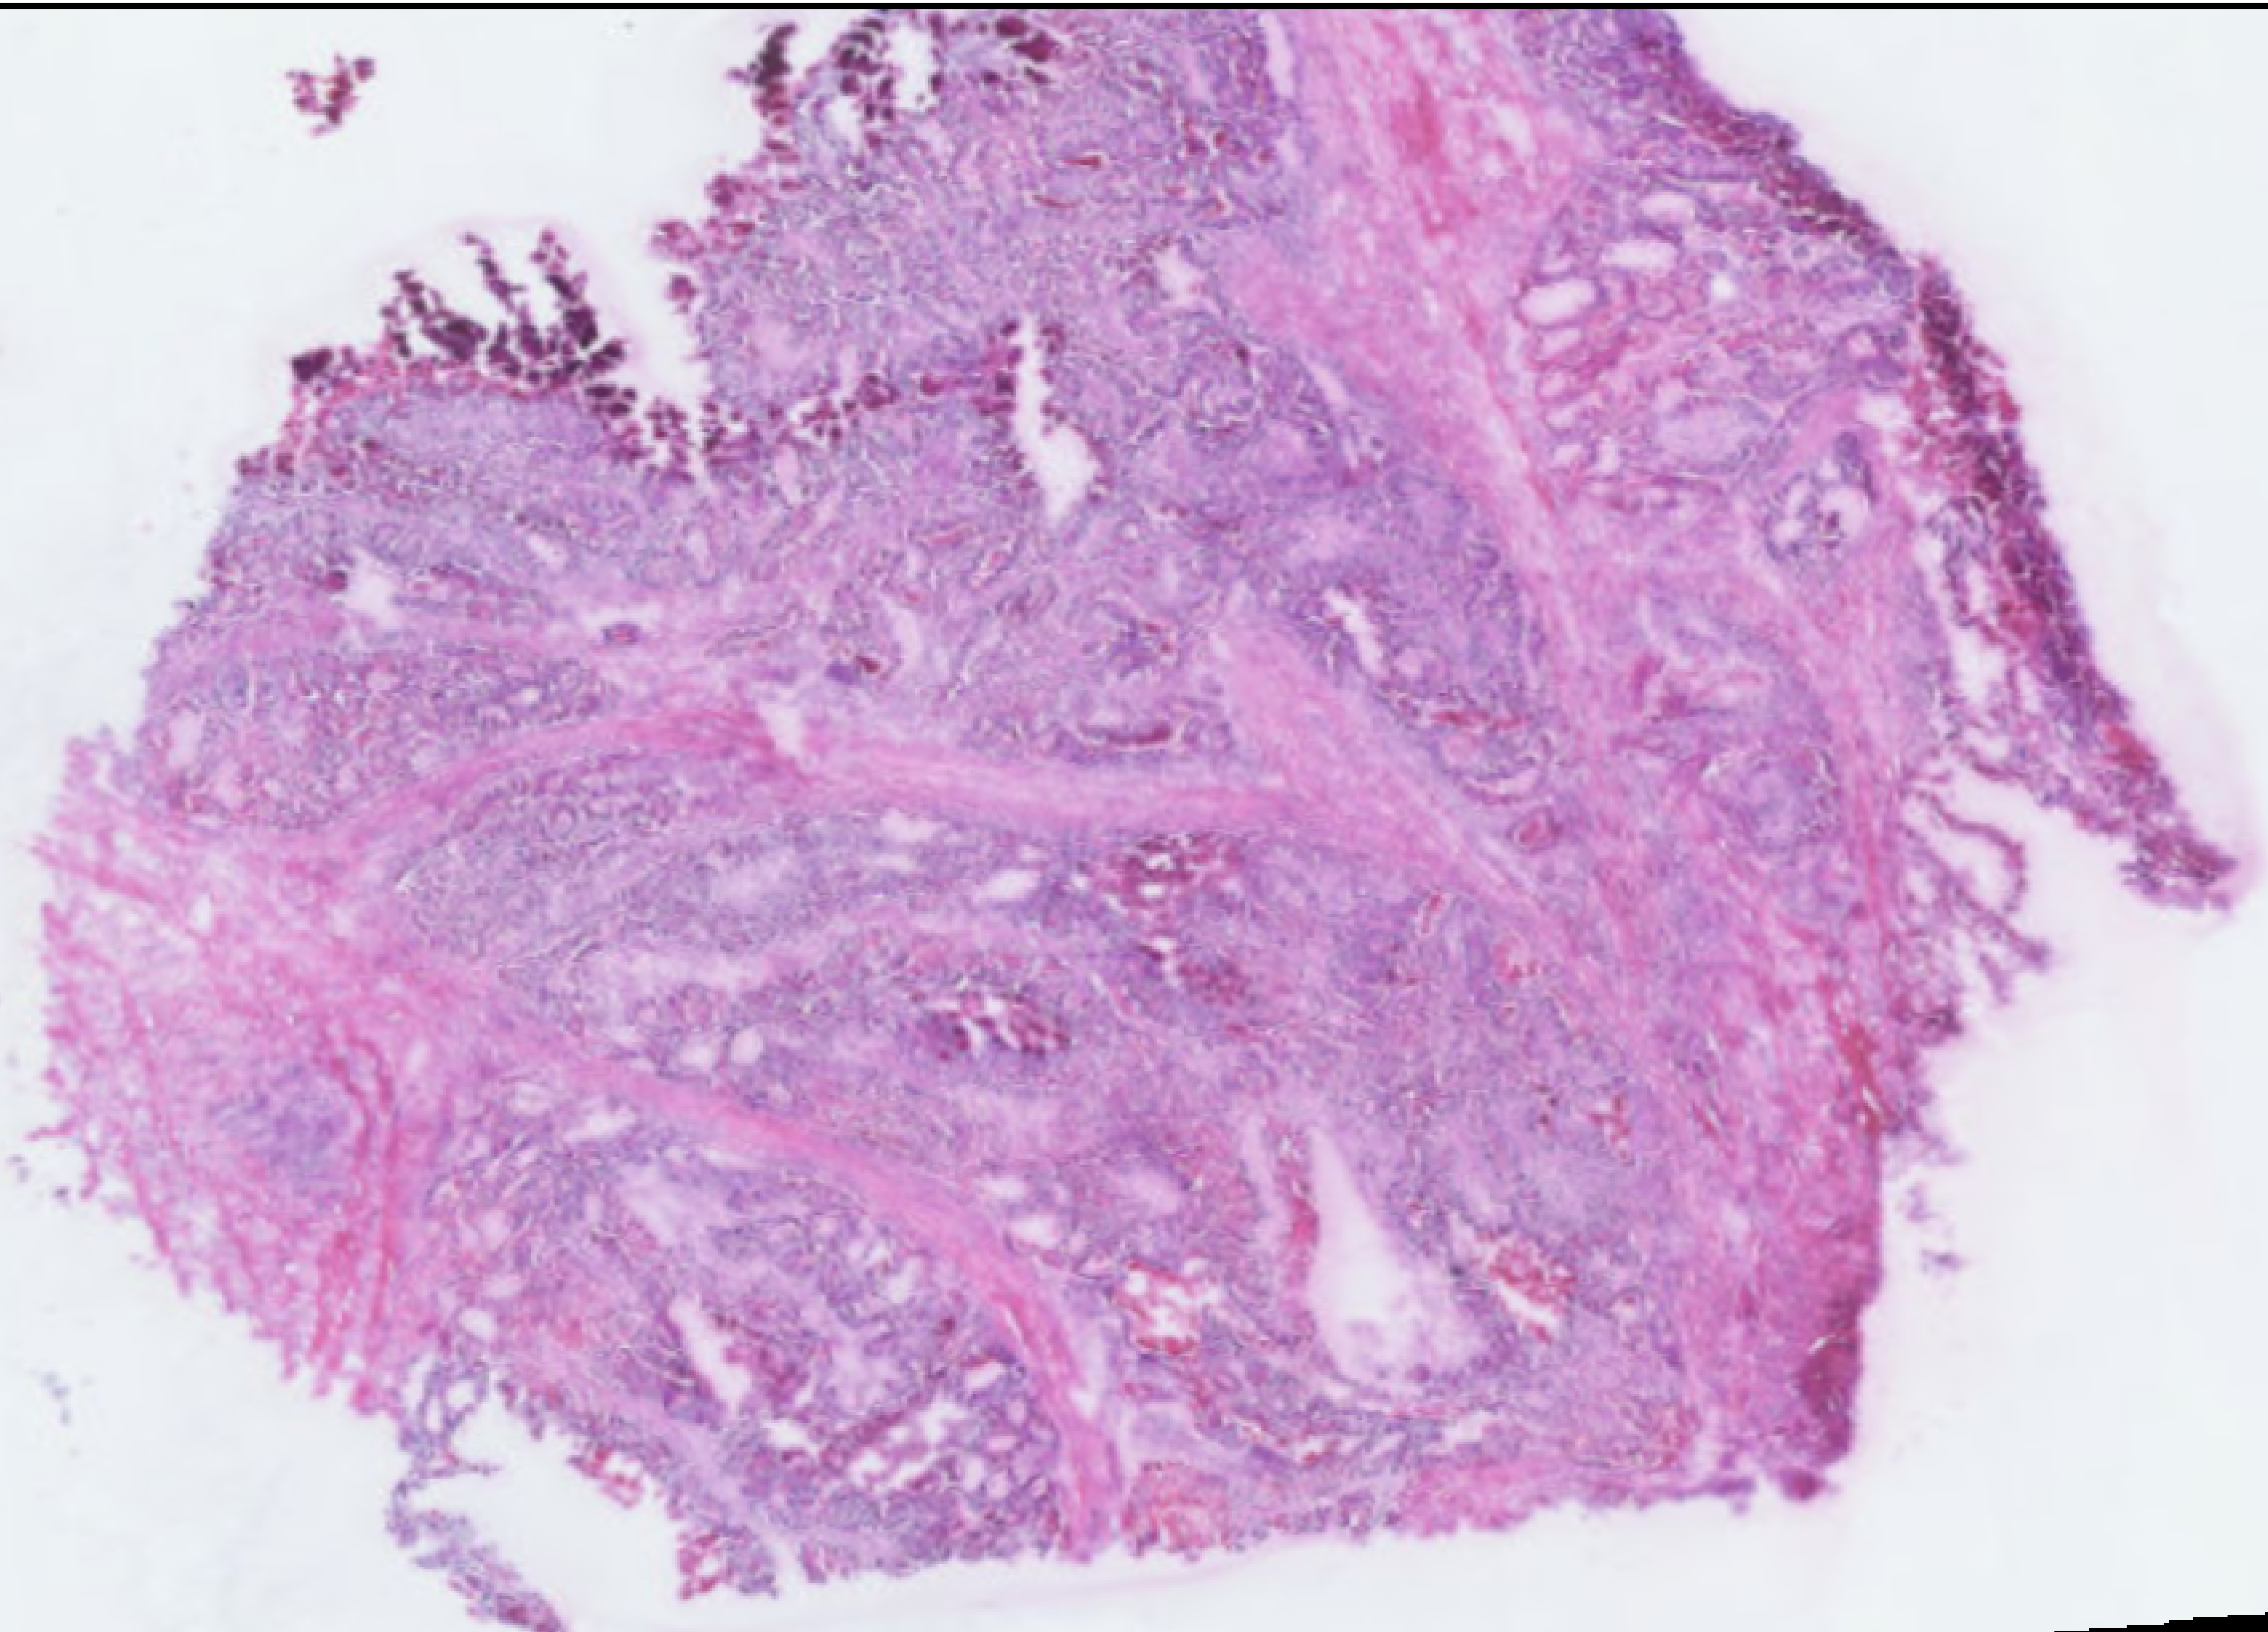
\includegraphics[width=\colWidth\textwidth]{pic/colorectal/s24_op.png}
  %   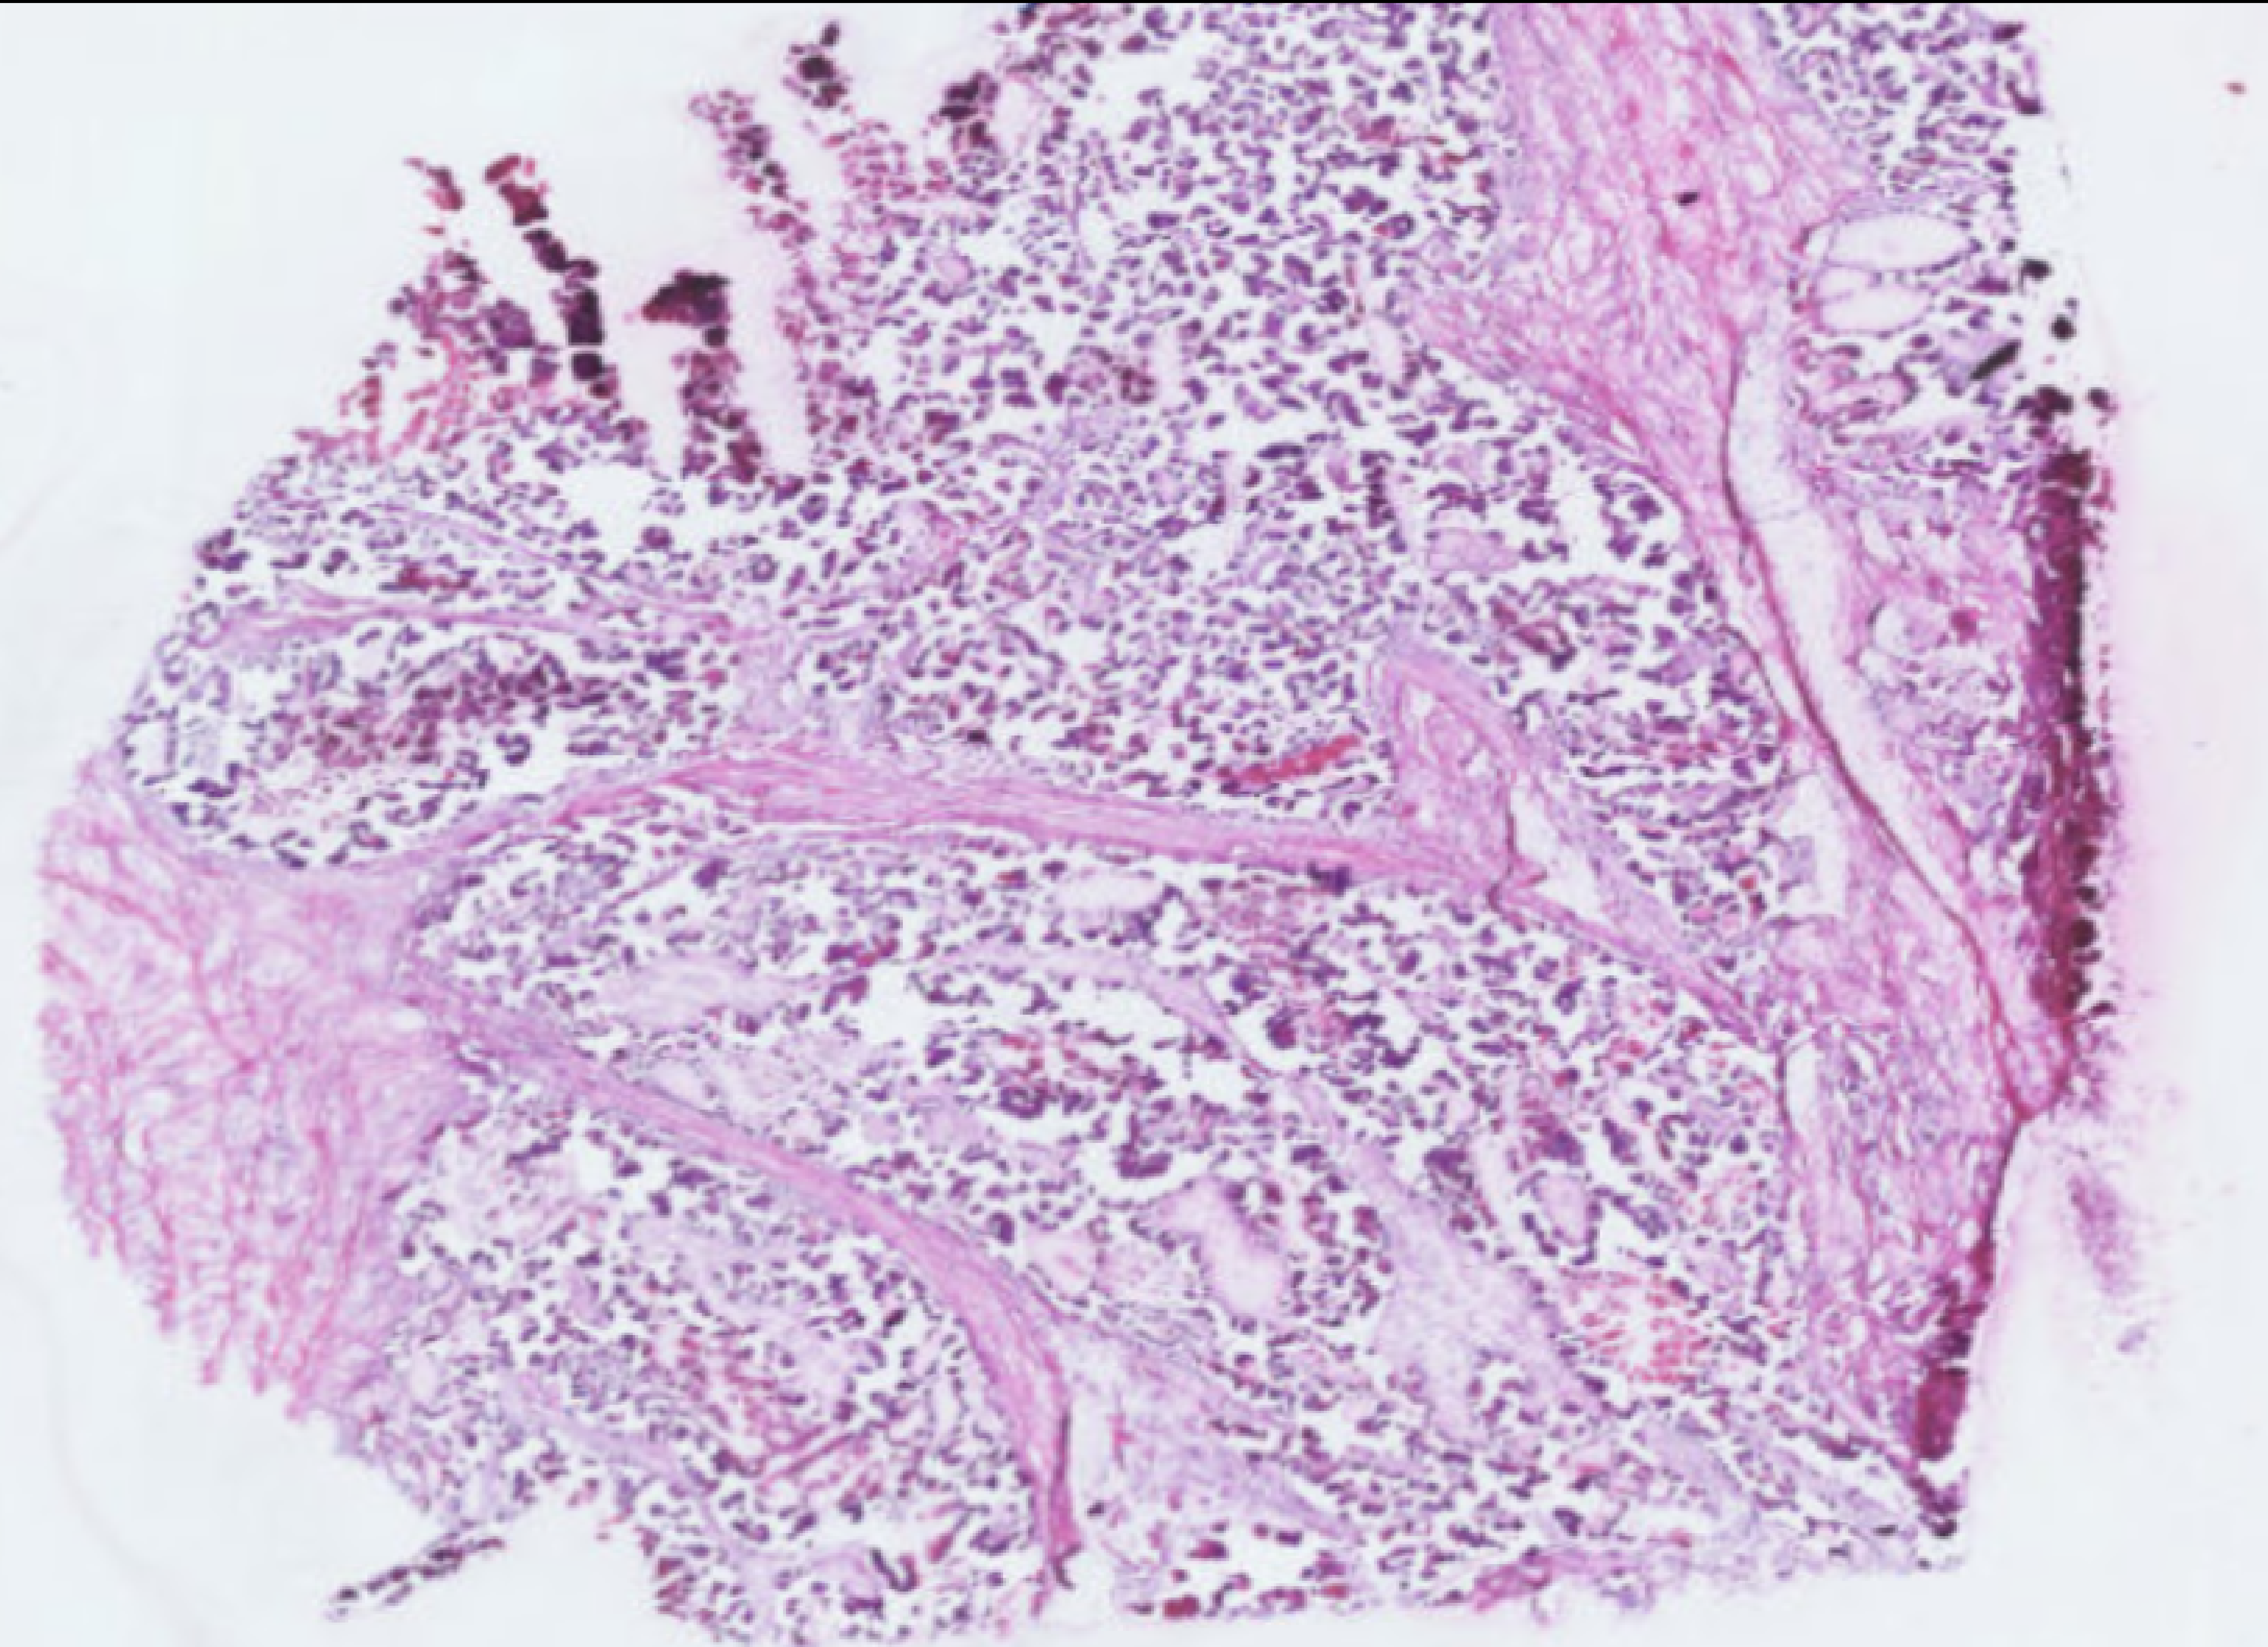
\includegraphics[width=\colWidth\textwidth]{pic/colorectal/s25_op.png}
  % } 
  % \end{minipage}
  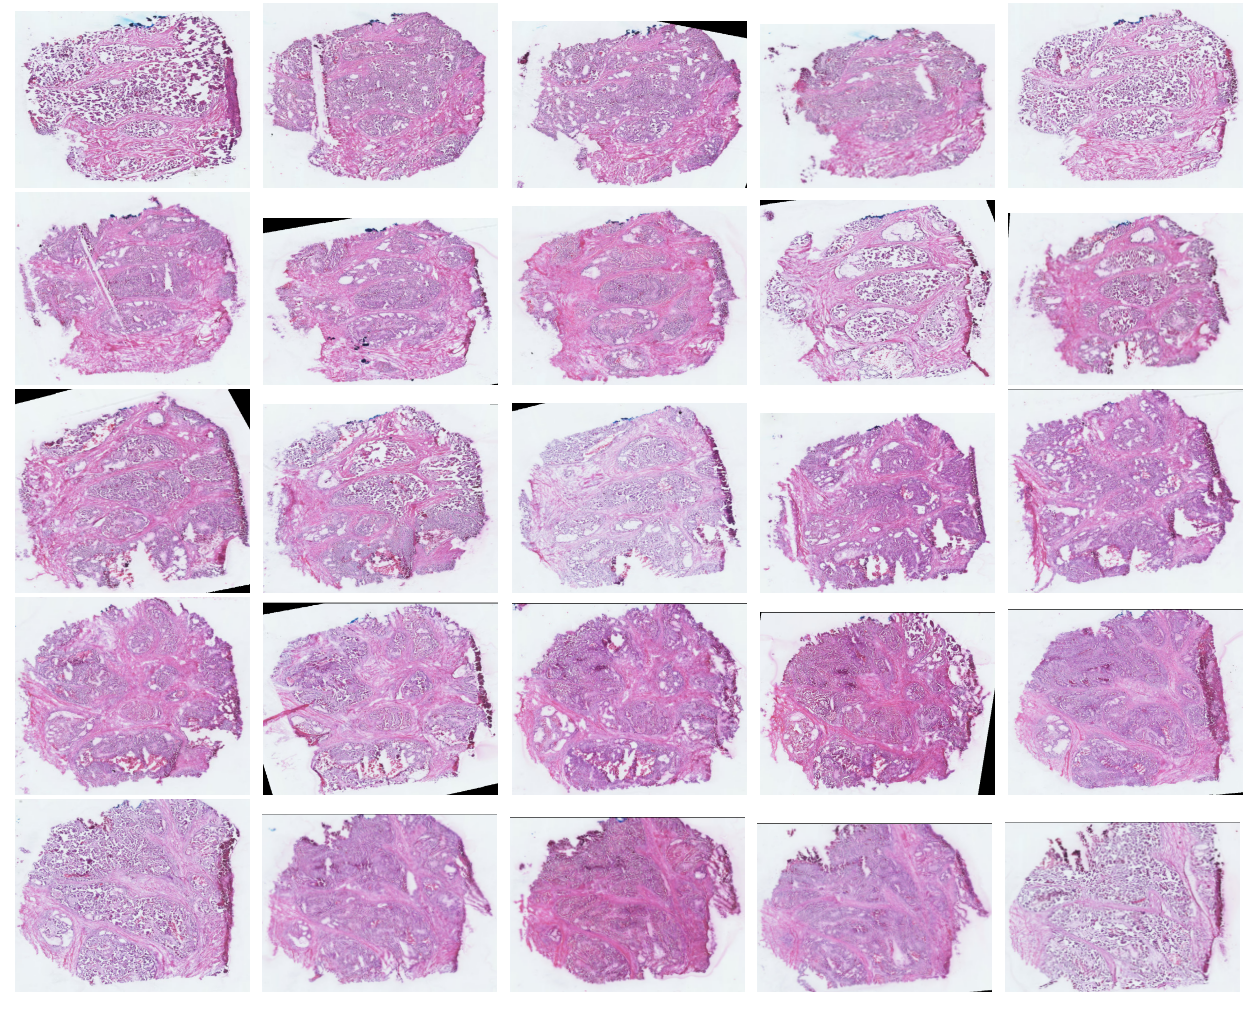
\includegraphics[width=\textwidth]{pic/all_op.png}
  \captionsetup{justification=raggedright,singlelinecheck=false}
  \caption{\textbf{H\&E stained patterns of colorectal adenocarcinoma dataset (25 sections)}.} 
  \label{fig:op of colorectal adenocarcinoma dataset} 
\end{figure}
 

\newcommand{\colWidth}{0.19}
\begin{figure}[htbp]
  \centering
    % \begin{minipage}[c]{0.9\textwidth}
    % {
    %   
\includegraphics[width=\colWidth\textwidth]{pic/colorectal/s1_cluster.png}
    %   
\includegraphics[width=\colWidth\textwidth]{pic/colorectal/s2_cluster.png}
    %   
\includegraphics[width=\colWidth\textwidth]{pic/colorectal/s3_cluster.png}
    %   
\includegraphics[width=\colWidth\textwidth]{pic/colorectal/s4_cluster.png}
    %   
\includegraphics[width=\colWidth\textwidth]{pic/colorectal/s5_cluster.png}
    %   \\
    %   
\includegraphics[width=\colWidth\textwidth]{pic/colorectal/s6_cluster.png}
    %   
\includegraphics[width=\colWidth\textwidth]{pic/colorectal/s7_cluster.png}
    %   
\includegraphics[width=\colWidth\textwidth]{pic/colorectal/s8_cluster.png}
    %   
\includegraphics[width=\colWidth\textwidth]{pic/colorectal/s9_cluster.png}
    %   
\includegraphics[width=\colWidth\textwidth]{pic/colorectal/s10_cluster.png}
    %   \\
    %   
\includegraphics[width=\colWidth\textwidth]{pic/colorectal/s11_cluster.png}
    %   
\includegraphics[width=\colWidth\textwidth]{pic/colorectal/s12_cluster.png}
    %   
\includegraphics[width=\colWidth\textwidth]{pic/colorectal/s13_cluster.png}
    %   
\includegraphics[width=\colWidth\textwidth]{pic/colorectal/s14_cluster.png}
    %   
\includegraphics[width=\colWidth\textwidth]{pic/colorectal/s15_cluster.png}
    %   \\
    %   \includegraphics[width=\colWidth\textwidth]{pic/colorectal/s16_cluster.png}
    %   \includegraphics[width=\colWidth\textwidth]{pic/colorectal/s17_cluster.png}
    %   \includegraphics[width=\colWidth\textwidth]{pic/colorectal/s18_cluster.png}
    %   \includegraphics[width=\colWidth\textwidth]{pic/colorectal/s19_cluster.png}
    %   \includegraphics[width=\colWidth\textwidth]{pic/colorectal/s20_cluster.png}
    %   \\
    %   \includegraphics[width=\colWidth\textwidth]{pic/colorectal/s21_cluster.png}
    %   \includegraphics[width=\colWidth\textwidth]{pic/colorectal/s22_cluster.png}
    %   \includegraphics[width=\colWidth\textwidth]{pic/colorectal/s23_cluster.png}
    %   \includegraphics[width=\colWidth\textwidth]{pic/colorectal/s24_cluster.png}
    %   \includegraphics[width=\colWidth\textwidth]{pic/colorectal/s25_cluster.png}
    % } 
    % \end{minipage}
    \includegraphics[width=\textwidth]{pic/clusters_all_sections.png}
    \captionsetup{justification=raggedright,singlelinecheck=false}
    \caption{
      \textbf{Clustering results of colorectal adenocarcinoma dataset (25 sections)}. 
      Tumor (blue) and connective tissue 
      clusters (yellow) are selected from the 
      clustered image which is derived 
      from the encoded features using a Gaussian mixture model 
      (k=5). These structures exhibit 
      a notable resemblance to their corresponding regions in the H\&E 
      histology, as indicated in Supplementary Figure 
      \ref{fig:op of colorectal adenocarcinoma dataset}.
      }
    \label{fig:Clusters of colorectal adenocarcinoma dataset}
\end{figure}

\begin{figure}[htbp]
  \centering
  % \begin{minipage}[c]{0.9\textwidth}
  %   {
  %     \includegraphics[width=\colWidth\textwidth]{pic/colorectal/s1_tumor.png}
  %     \includegraphics[width=\colWidth\textwidth]{pic/colorectal/s2_tumor.png}
  %     \includegraphics[width=\colWidth\textwidth]{pic/colorectal/s3_tumor.png}
  %     \includegraphics[width=\colWidth\textwidth]{pic/colorectal/s4_tumor.png}
  %     \includegraphics[width=\colWidth\textwidth]{pic/colorectal/s5_tumor.png}
  %     \\
  %     \includegraphics[width=\colWidth\textwidth]{pic/colorectal/s6_tumor.png}
  %     \includegraphics[width=\colWidth\textwidth]{pic/colorectal/s7_tumor.png}
  %     \includegraphics[width=\colWidth\textwidth]{pic/colorectal/s8_tumor.png}
  %     \includegraphics[width=\colWidth\textwidth]{pic/colorectal/s9_tumor.png}
  %     \includegraphics[width=\colWidth\textwidth]{pic/colorectal/s10_tumor.png}
  %     \\
  %     \includegraphics[width=\colWidth\textwidth]{pic/colorectal/s11_tumor.png}
  %     \includegraphics[width=\colWidth\textwidth]{pic/colorectal/s12_tumor.png}
  %     \includegraphics[width=\colWidth\textwidth]{pic/colorectal/s13_tumor.png}
  %     \includegraphics[width=\colWidth\textwidth]{pic/colorectal/s14_tumor.png}
  %     \includegraphics[width=\colWidth\textwidth]{pic/colorectal/s15_tumor.png}
  %     \\
  %     \includegraphics[width=\colWidth\textwidth]{pic/colorectal/s16_tumor.png}
  %     \includegraphics[width=\colWidth\textwidth]{pic/colorectal/s17_tumor.png}
  %     \includegraphics[width=\colWidth\textwidth]{pic/colorectal/s18_tumor.png}
  %     \includegraphics[width=\colWidth\textwidth]{pic/colorectal/s19_tumor.png}
  %     \includegraphics[width=\colWidth\textwidth]{pic/colorectal/s20_tumor.png}
  %     \\
  %     \includegraphics[width=\colWidth\textwidth]{pic/colorectal/s21_tumor.png}
  %     \includegraphics[width=\colWidth\textwidth]{pic/colorectal/s22_tumor.png}
  %     \includegraphics[width=\colWidth\textwidth]{pic/colorectal/s23_tumor.png}
  %     \includegraphics[width=\colWidth\textwidth]{pic/colorectal/s24_tumor.png}
  %     \includegraphics[width=\colWidth\textwidth]{pic/colorectal/s25_tumor.png}
  %   } 
  % \end{minipage}
  \includegraphics[width=\textwidth]{pic/mzs_all_clusters.png}
  \captionsetup{justification=raggedright,singlelinecheck=false}
  \caption{
    \textbf{The spatial distribution of the ion feature most highly correlated with the tumor cluster is found at m/z 720.49, 
    with a Pearson correlation coefficient of 0.79.}
    }
  \label{fig:tumor colorectal adenocarcinoma dataset}
\end{figure}



\end{document}

